% Options for packages loaded elsewhere
\PassOptionsToPackage{unicode}{hyperref}
\PassOptionsToPackage{hyphens}{url}
%
\documentclass[
]{article}
\usepackage{amsmath,amssymb}
\usepackage{lmodern}
\usepackage{iftex}
\ifPDFTeX
  \usepackage[T1]{fontenc}
  \usepackage[utf8]{inputenc}
  \usepackage{textcomp} % provide euro and other symbols
\else % if luatex or xetex
  \usepackage{unicode-math}
  \defaultfontfeatures{Scale=MatchLowercase}
  \defaultfontfeatures[\rmfamily]{Ligatures=TeX,Scale=1}
\fi
% Use upquote if available, for straight quotes in verbatim environments
\IfFileExists{upquote.sty}{\usepackage{upquote}}{}
\IfFileExists{microtype.sty}{% use microtype if available
  \usepackage[]{microtype}
  \UseMicrotypeSet[protrusion]{basicmath} % disable protrusion for tt fonts
}{}
\makeatletter
\@ifundefined{KOMAClassName}{% if non-KOMA class
  \IfFileExists{parskip.sty}{%
    \usepackage{parskip}
  }{% else
    \setlength{\parindent}{0pt}
    \setlength{\parskip}{6pt plus 2pt minus 1pt}}
}{% if KOMA class
  \KOMAoptions{parskip=half}}
\makeatother
\usepackage{xcolor}
\usepackage[margin=1in]{geometry}
\usepackage{graphicx}
\makeatletter
\def\maxwidth{\ifdim\Gin@nat@width>\linewidth\linewidth\else\Gin@nat@width\fi}
\def\maxheight{\ifdim\Gin@nat@height>\textheight\textheight\else\Gin@nat@height\fi}
\makeatother
% Scale images if necessary, so that they will not overflow the page
% margins by default, and it is still possible to overwrite the defaults
% using explicit options in \includegraphics[width, height, ...]{}
\setkeys{Gin}{width=\maxwidth,height=\maxheight,keepaspectratio}
% Set default figure placement to htbp
\makeatletter
\def\fps@figure{htbp}
\makeatother
\setlength{\emergencystretch}{3em} % prevent overfull lines
\providecommand{\tightlist}{%
  \setlength{\itemsep}{0pt}\setlength{\parskip}{0pt}}
\setcounter{secnumdepth}{-\maxdimen} % remove section numbering
\newlength{\cslhangindent}
\setlength{\cslhangindent}{1.5em}
\newlength{\csllabelwidth}
\setlength{\csllabelwidth}{3em}
\newlength{\cslentryspacingunit} % times entry-spacing
\setlength{\cslentryspacingunit}{\parskip}
\newenvironment{CSLReferences}[2] % #1 hanging-ident, #2 entry spacing
 {% don't indent paragraphs
  \setlength{\parindent}{0pt}
  % turn on hanging indent if param 1 is 1
  \ifodd #1
  \let\oldpar\par
  \def\par{\hangindent=\cslhangindent\oldpar}
  \fi
  % set entry spacing
  \setlength{\parskip}{#2\cslentryspacingunit}
 }%
 {}
\usepackage{calc}
\newcommand{\CSLBlock}[1]{#1\hfill\break}
\newcommand{\CSLLeftMargin}[1]{\parbox[t]{\csllabelwidth}{#1}}
\newcommand{\CSLRightInline}[1]{\parbox[t]{\linewidth - \csllabelwidth}{#1}\break}
\newcommand{\CSLIndent}[1]{\hspace{\cslhangindent}#1}
\usepackage{float}
\ifLuaTeX
  \usepackage{selnolig}  % disable illegal ligatures
\fi
\IfFileExists{bookmark.sty}{\usepackage{bookmark}}{\usepackage{hyperref}}
\IfFileExists{xurl.sty}{\usepackage{xurl}}{} % add URL line breaks if available
\urlstyle{same} % disable monospaced font for URLs
\hypersetup{
  pdftitle={Assessment for WKBANSP 2024 using age-structured data in SS3: Anchovy in ICES Subdivision 9a South (ane.27.9a Southern component)},
  hidelinks,
  pdfcreator={LaTeX via pandoc}}

\title{Assessment for WKBANSP 2024 using age-structured data in SS3:
Anchovy in ICES Subdivision 9a South (ane.27.9a Southern component)}
\author{María José
Zúñiga\thanks{Centro Oceanográfico de Cádiz (COCAD-IEO), CSIC},
Margarita María
Rincón\thanks{Centro Oceanográfico de Cádiz (COCAD-IEO), CSIC}, Fernando
Ramos\thanks{Centro Oceanográfico de Cádiz (COCAD-IEO), CSIC}}
\date{}

\begin{document}
\maketitle

\hypertarget{assessment-model}{%
\section{Assessment model}\label{assessment-model}}

The assessment of the anchovy in ICES division 9a, southern component
was performed in Stock Synthesis software, version 3.30.22.1 (SS3,
Methot \emph{et al.}, 2024) under the Linux platform. SS3 is a
generalized age and/or length-based model that is very flexible with
regard to the types of data that may be included, the functional forms
that are used for various biological processes, the level of complexity
and number of parameters that may be estimated. The model is coded in
C++ with parameter estimation enabled by automatic differentiation
(www.admb-project.org) and available at the NOAA Fisheries integrated
toolbox: \url{https://noaa-fisheries-integrated-toolbox.github.io/SS3}.
A description and discussion of the model can be found in Methot and
Wetzel (2013).

The model is defined quarterly between 1989 and 2023, for one area and
it is age-based, where the population is comprised of 3+ age-classes
(with age 3 representing a plus group) with sexes combined (male and
females are modelled together).

\hypertarget{data}{%
\section{Data}\label{data}}

Input data include total catch (in biomass), age composition of the
catch (in proportion), abundance (in biomass) and age composition from
three annual surveys: \emph{PELAGO}, \emph{ECOCADIZ} and
\emph{ECOCADIZ-RECLUTAS}; and spawning-stock biomass (SSB) estimates
from a triennial DEPM \emph{BOCADEVA} survey. The Figure 1 provides a
visual representation of the input data used in the model, categorized
into three main types: catches, abundance indices, and age compositions.
These data are displayed over time (years) and are represented by
circles, with the size of each circle reflecting the magnitude of the
data.

\begin{figure}[H]

{\centering 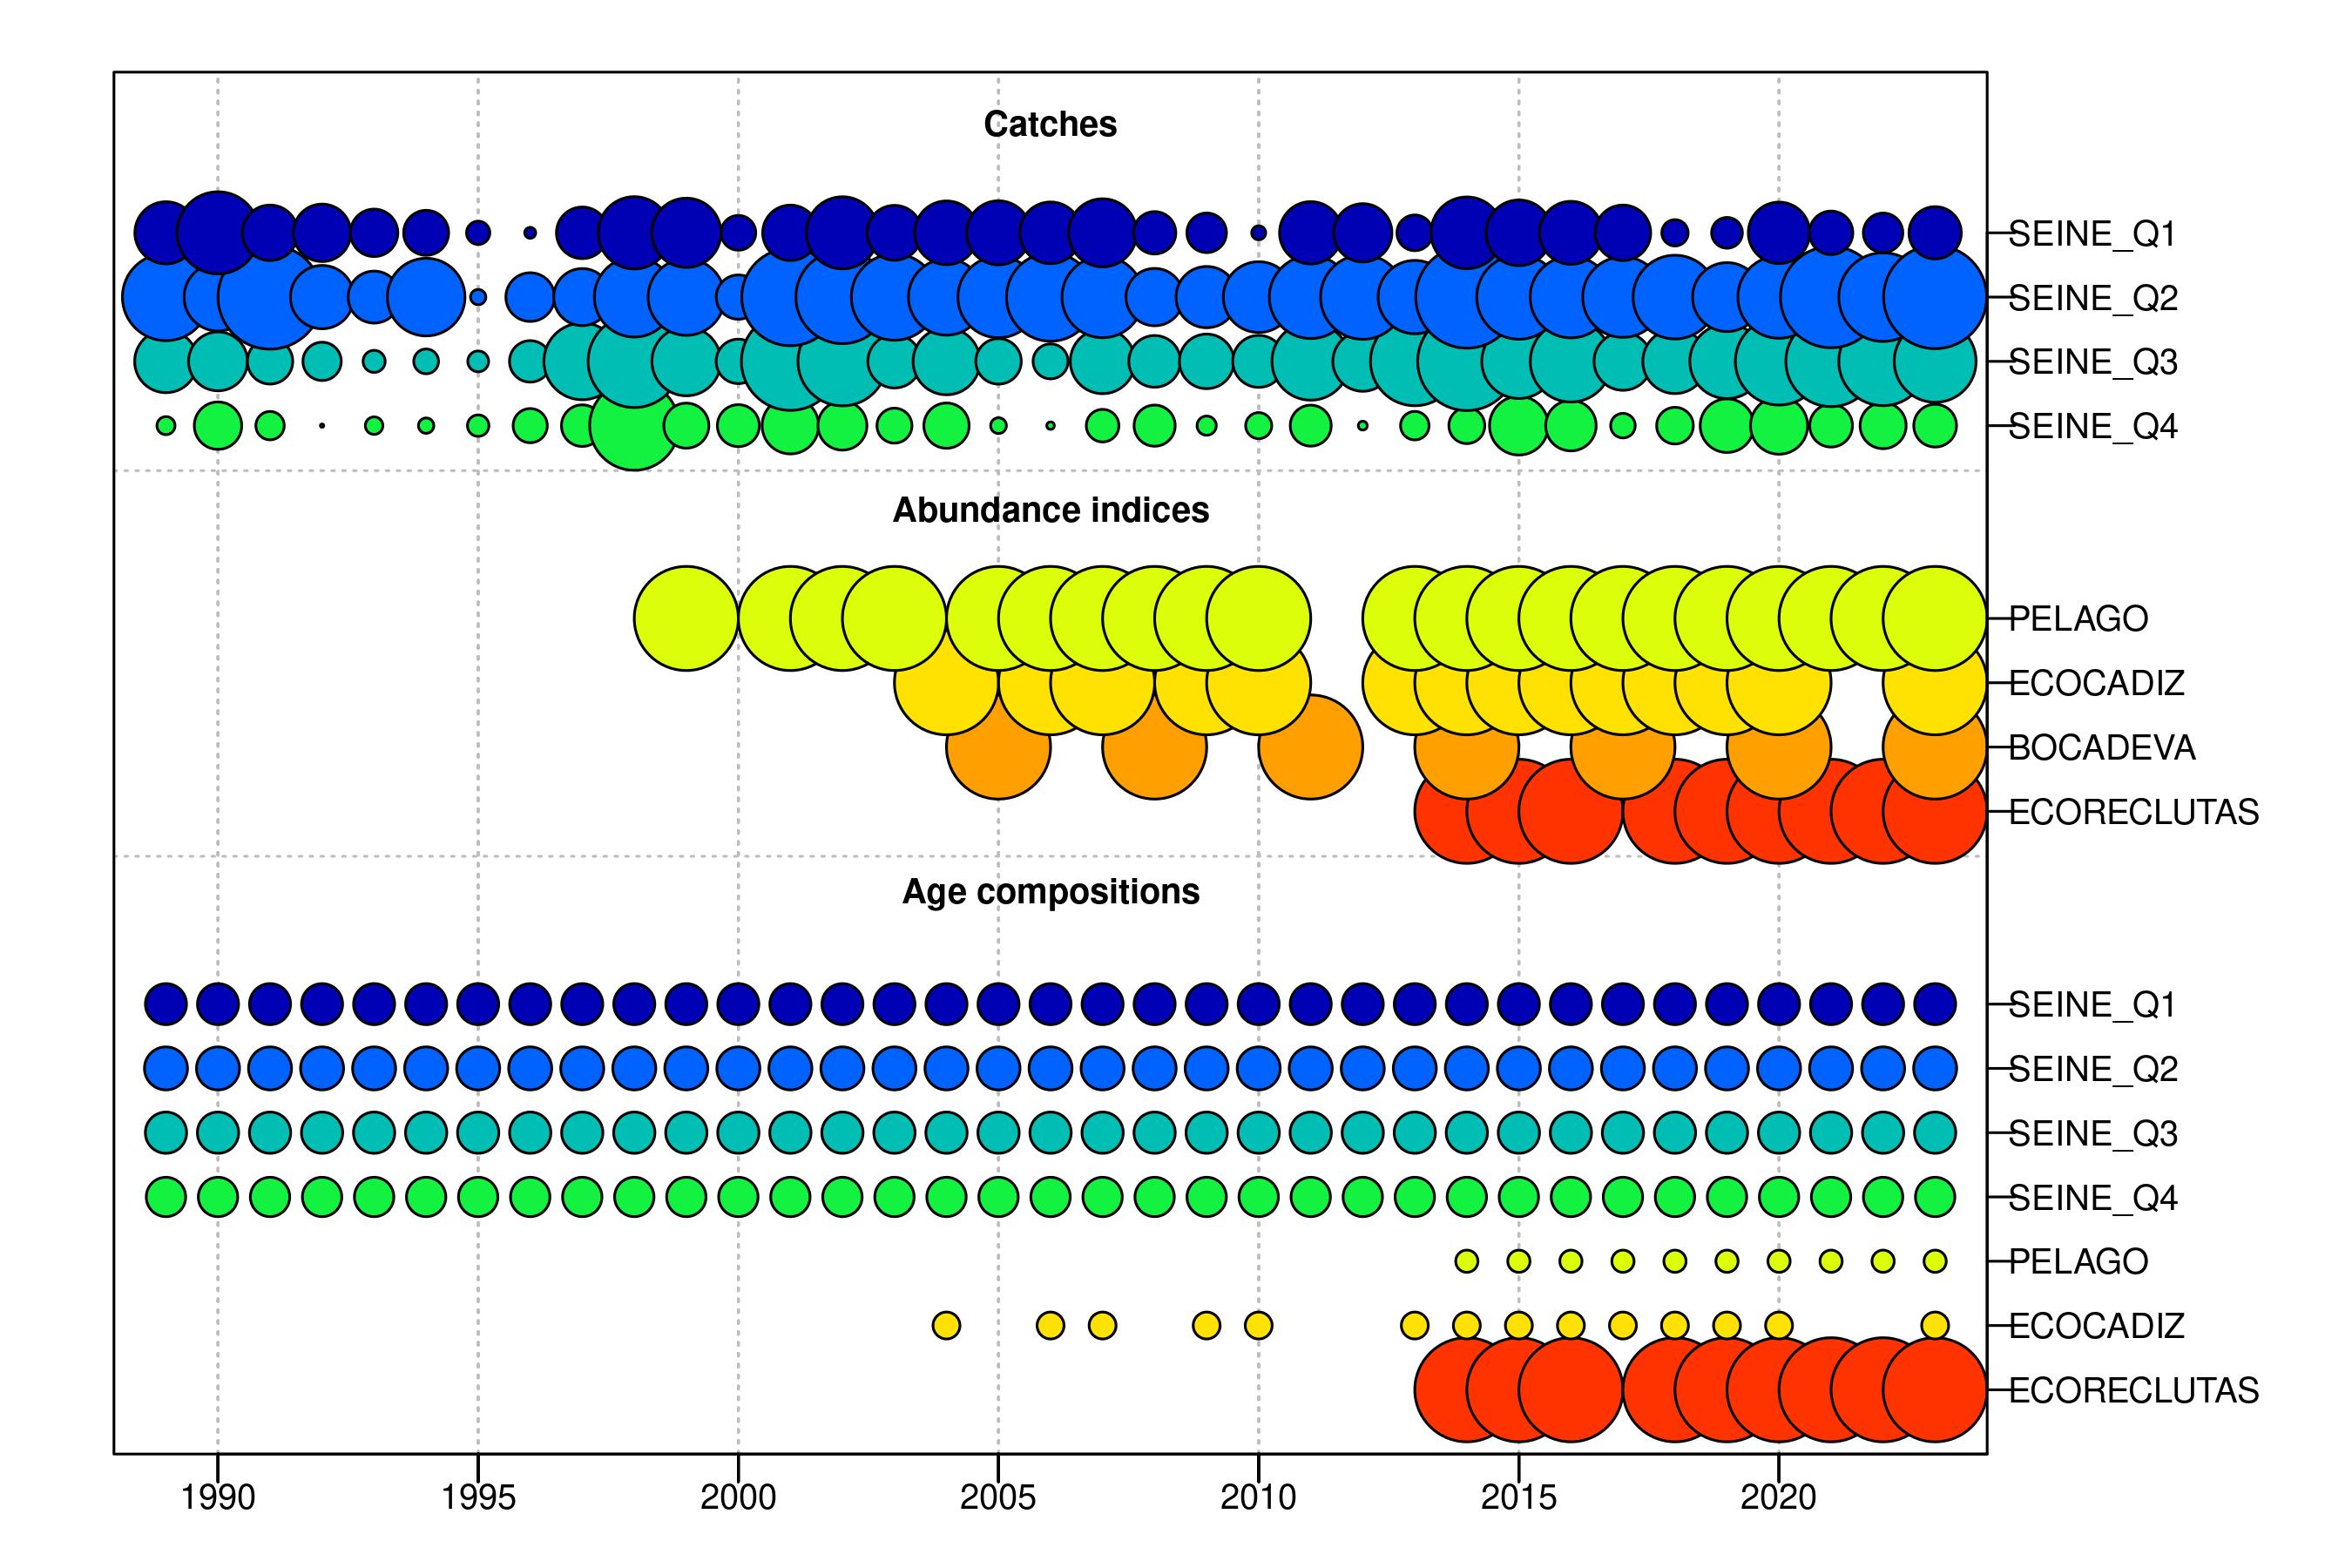
\includegraphics[width=0.95\linewidth]{report/run/S1.0_4FLEETS/fig_input_data} 

}

\caption{ane.27.9a stock. Summarises data input by year, where circle area is relative within a data type. Circles are proportional to total catch for catches, to precision for indices and to total sample size for age compositions.}\label{fig:unnamed-chunk-2}
\end{figure}

\hypertarget{catches}{%
\subsection{Catches}\label{catches}}

Anchovy catches in the Gulf of Cádiz exhibit seasonality, with 40.61\%
concentrated in the second quarter (Q2), averaging 2120.26 tons
historically, followed by the third quarter (Q3) with 29.60\% (1545.23
tons), the first quarter (Q1) with 19.39\% (1012.42 tons), and the
fourth quarter (Q4) with 10.39\% (542.61 tons). In 2023, first-quarter
catches were 7.84\% lower than the historical average, while second,
third, and fourth-quarter catches increased by 71.03\%, 48.06\%, and
14.70\%, respectively (Figures 2 and 3).

\begin{figure}[H]

{\centering 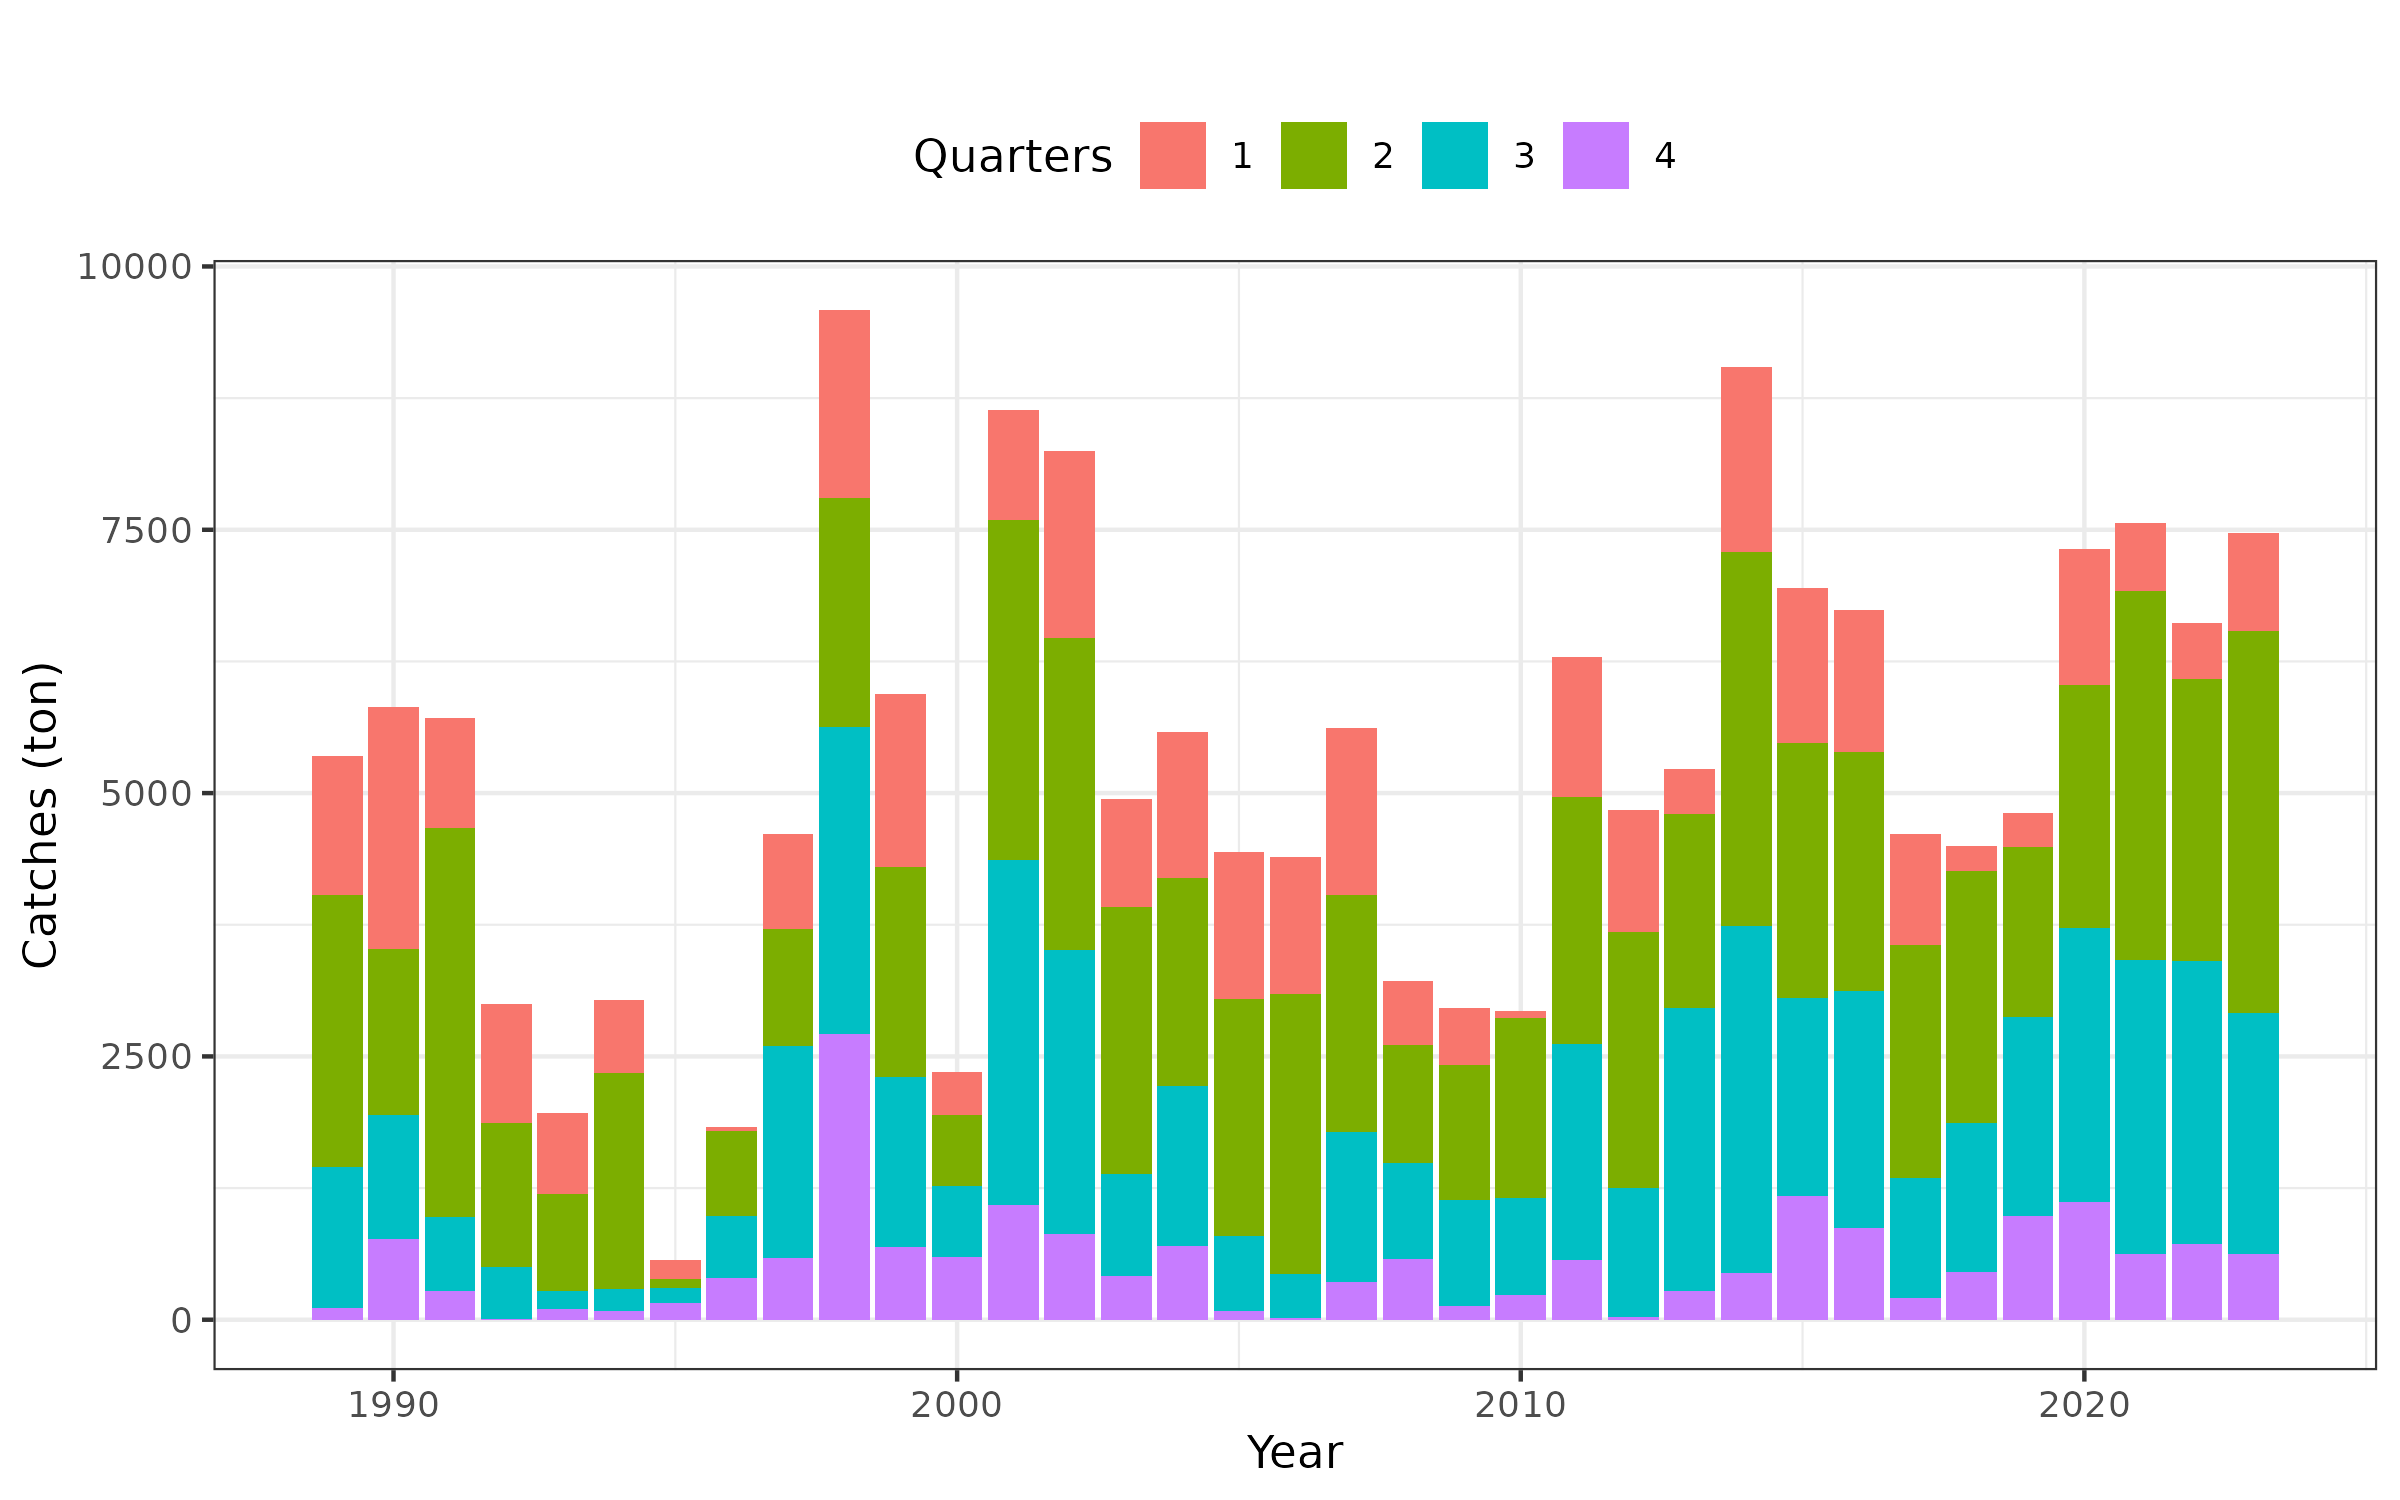
\includegraphics[width=0.95\linewidth]{report/run/S1.0_4FLEETS/fig_catches} 

}

\caption{ane.27.9a stock. Quarterly Catch.}\label{fig:unnamed-chunk-3}
\end{figure}

\begin{figure}[H]

{\centering 
\includegraphics[width=0.95\linewidth]{report/run/S1.0_4FLEETS/tb_catches} 

}

\caption{ane.27.9a stock. Quarterly Catch data. }\label{fig:unnamed-chunk-4}
\end{figure}

\hypertarget{abundance-indices}{%
\subsection{Abundance indices}\label{abundance-indices}}

The abundance indices \emph{PELAGO}, \emph{ECOCADIZ}, \emph{BOCADEVA},
and \emph{ECOCADIZ-RECLUTAS} exhibit interannual variability over time
(Figure 4). \emph{PELAGO}, with data from 1999 to 2023, shows
fluctuations with a peak in 2016 at 65,345 tons, followed by a decline,
but with a slight recovery in 2023 to 26,786 tons. \emph{ECOCADIZ},
covering the period from 2004 to 2023, reaches its maximum in 2019 at
57,700 tons, followed by a significant decrease to 9,714 tons in 2023.
\emph{BOCADEVA}, with data from 2005 to 2023, shows a steady increase to
its peak in 2020 at 81,466 tons, followed by a reduction to 15,138 tons
in 2023. \emph{ECOCADIZ-RECLUTAS}, recorded from 2014 to 2023, shows a
sustained increase until 2019 at 48,398 tons, followed by a decrease to
8,300 tons in 2023. These patterns reflect a high variability in
abundance over time with periods of increase followed by declines in the
later years of each series (Figure 4).

\begin{figure}[H]

{\centering 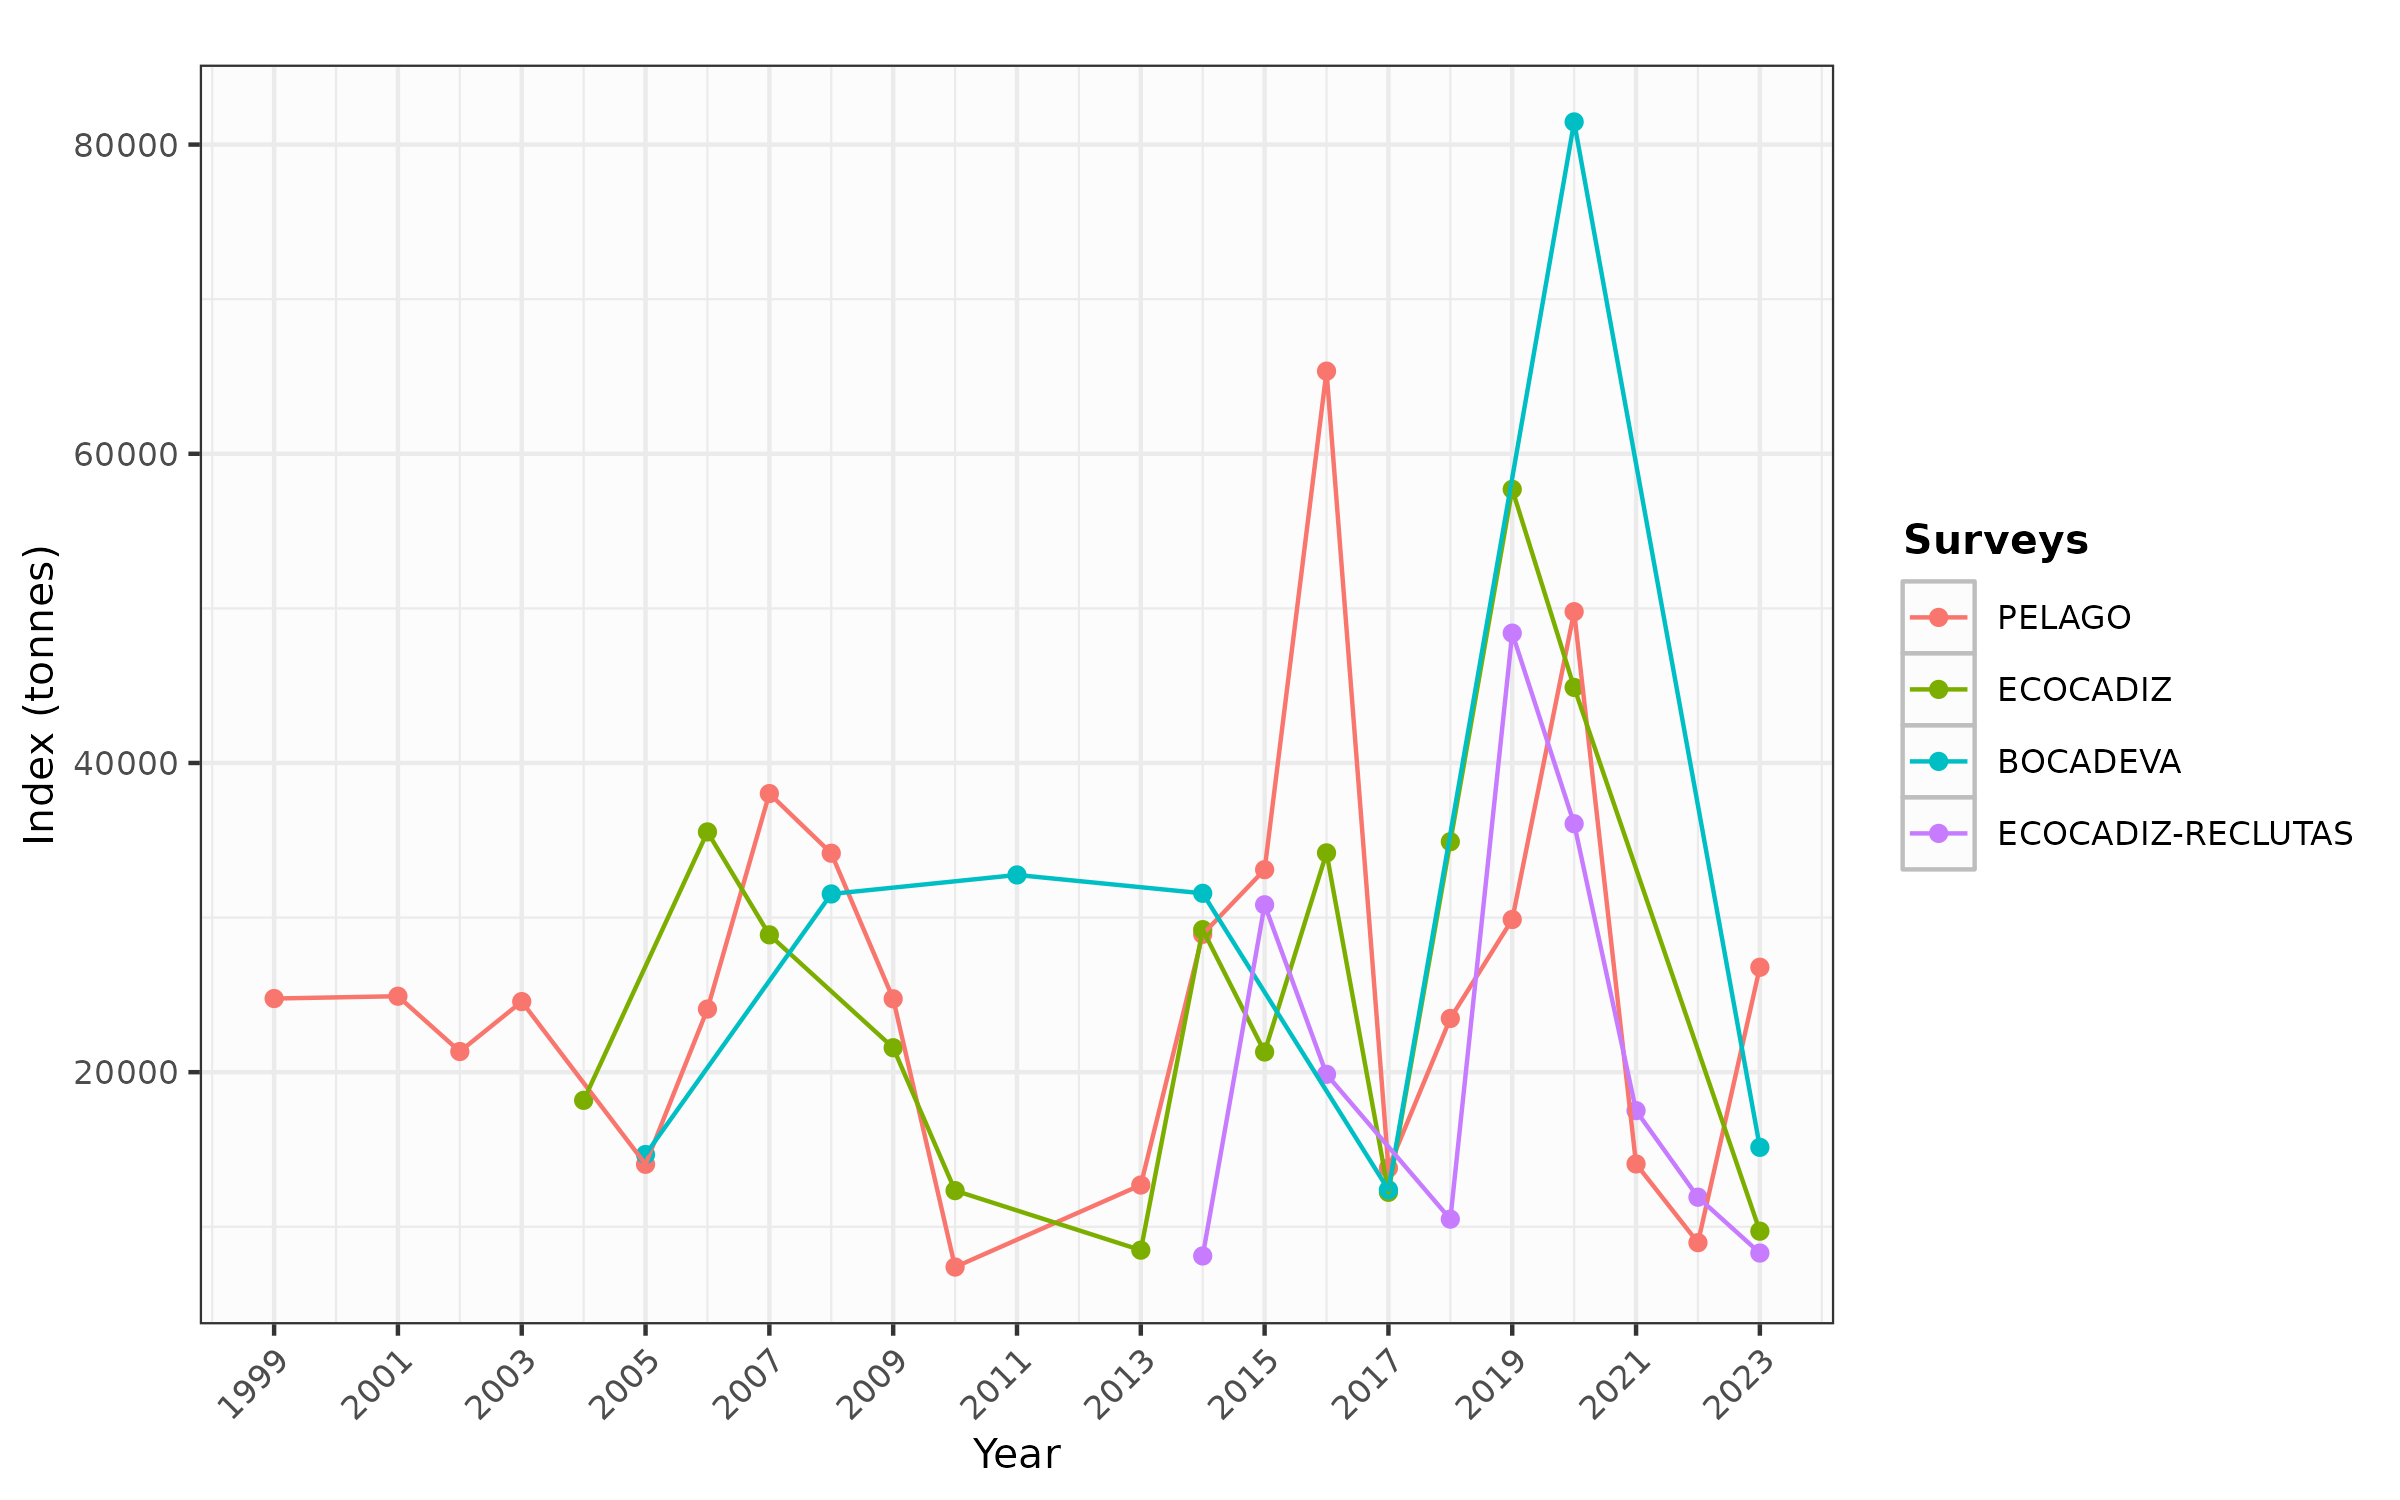
\includegraphics[width=0.95\linewidth]{report/run/S1.0_4FLEETS//fig_indiceBiomass} 

}

\caption{ane.27.9a stock. Time series of biomass indices for the Gulf of Cádiz anchovy stock, estimated by the PELAGO, ECOCADIZ, BOCADEVA, and ECOCADIZ-RECLUTAS surveys.}\label{fig:unnamed-chunk-5}
\end{figure}

\begin{figure}[H]

{\centering 
\includegraphics[width=0.95\linewidth]{report/run/S1.0_4FLEETS/tb_index} 

}

\caption{ane.27.9a stock. Acoustic biomass (ton) by surveys *PELAGO*, *ECOCADIZ*, *BOCADEVA*, and *ECOCADIZ-RECLUTAS*.   }\label{fig:unnamed-chunk-6}
\end{figure}

\hypertarget{age-composition}{%
\subsection{Age composition}\label{age-composition}}

In the model, the age proportion of the commercial fleet (\emph{SEINE})
by quarter from 1989 to 2023, is used (Figure 6). It can be observed,
that age-0 proportion compared to other ages has been increasing in the
last years while age-1 predominates in Q1 and Q2, with a constant
proportion over time. Age-0 is not recorded in Q1 and Q2 by convention.
In Q3 and Q4, the proportion of age-1 individuals decreases as the
proportion of age-0 increases. Additionally, ages 2 and 3 exhibit lower
and variable proportions across all quarters over the years, without a
defined pattern of change.

\begin{figure}[H]

{\centering 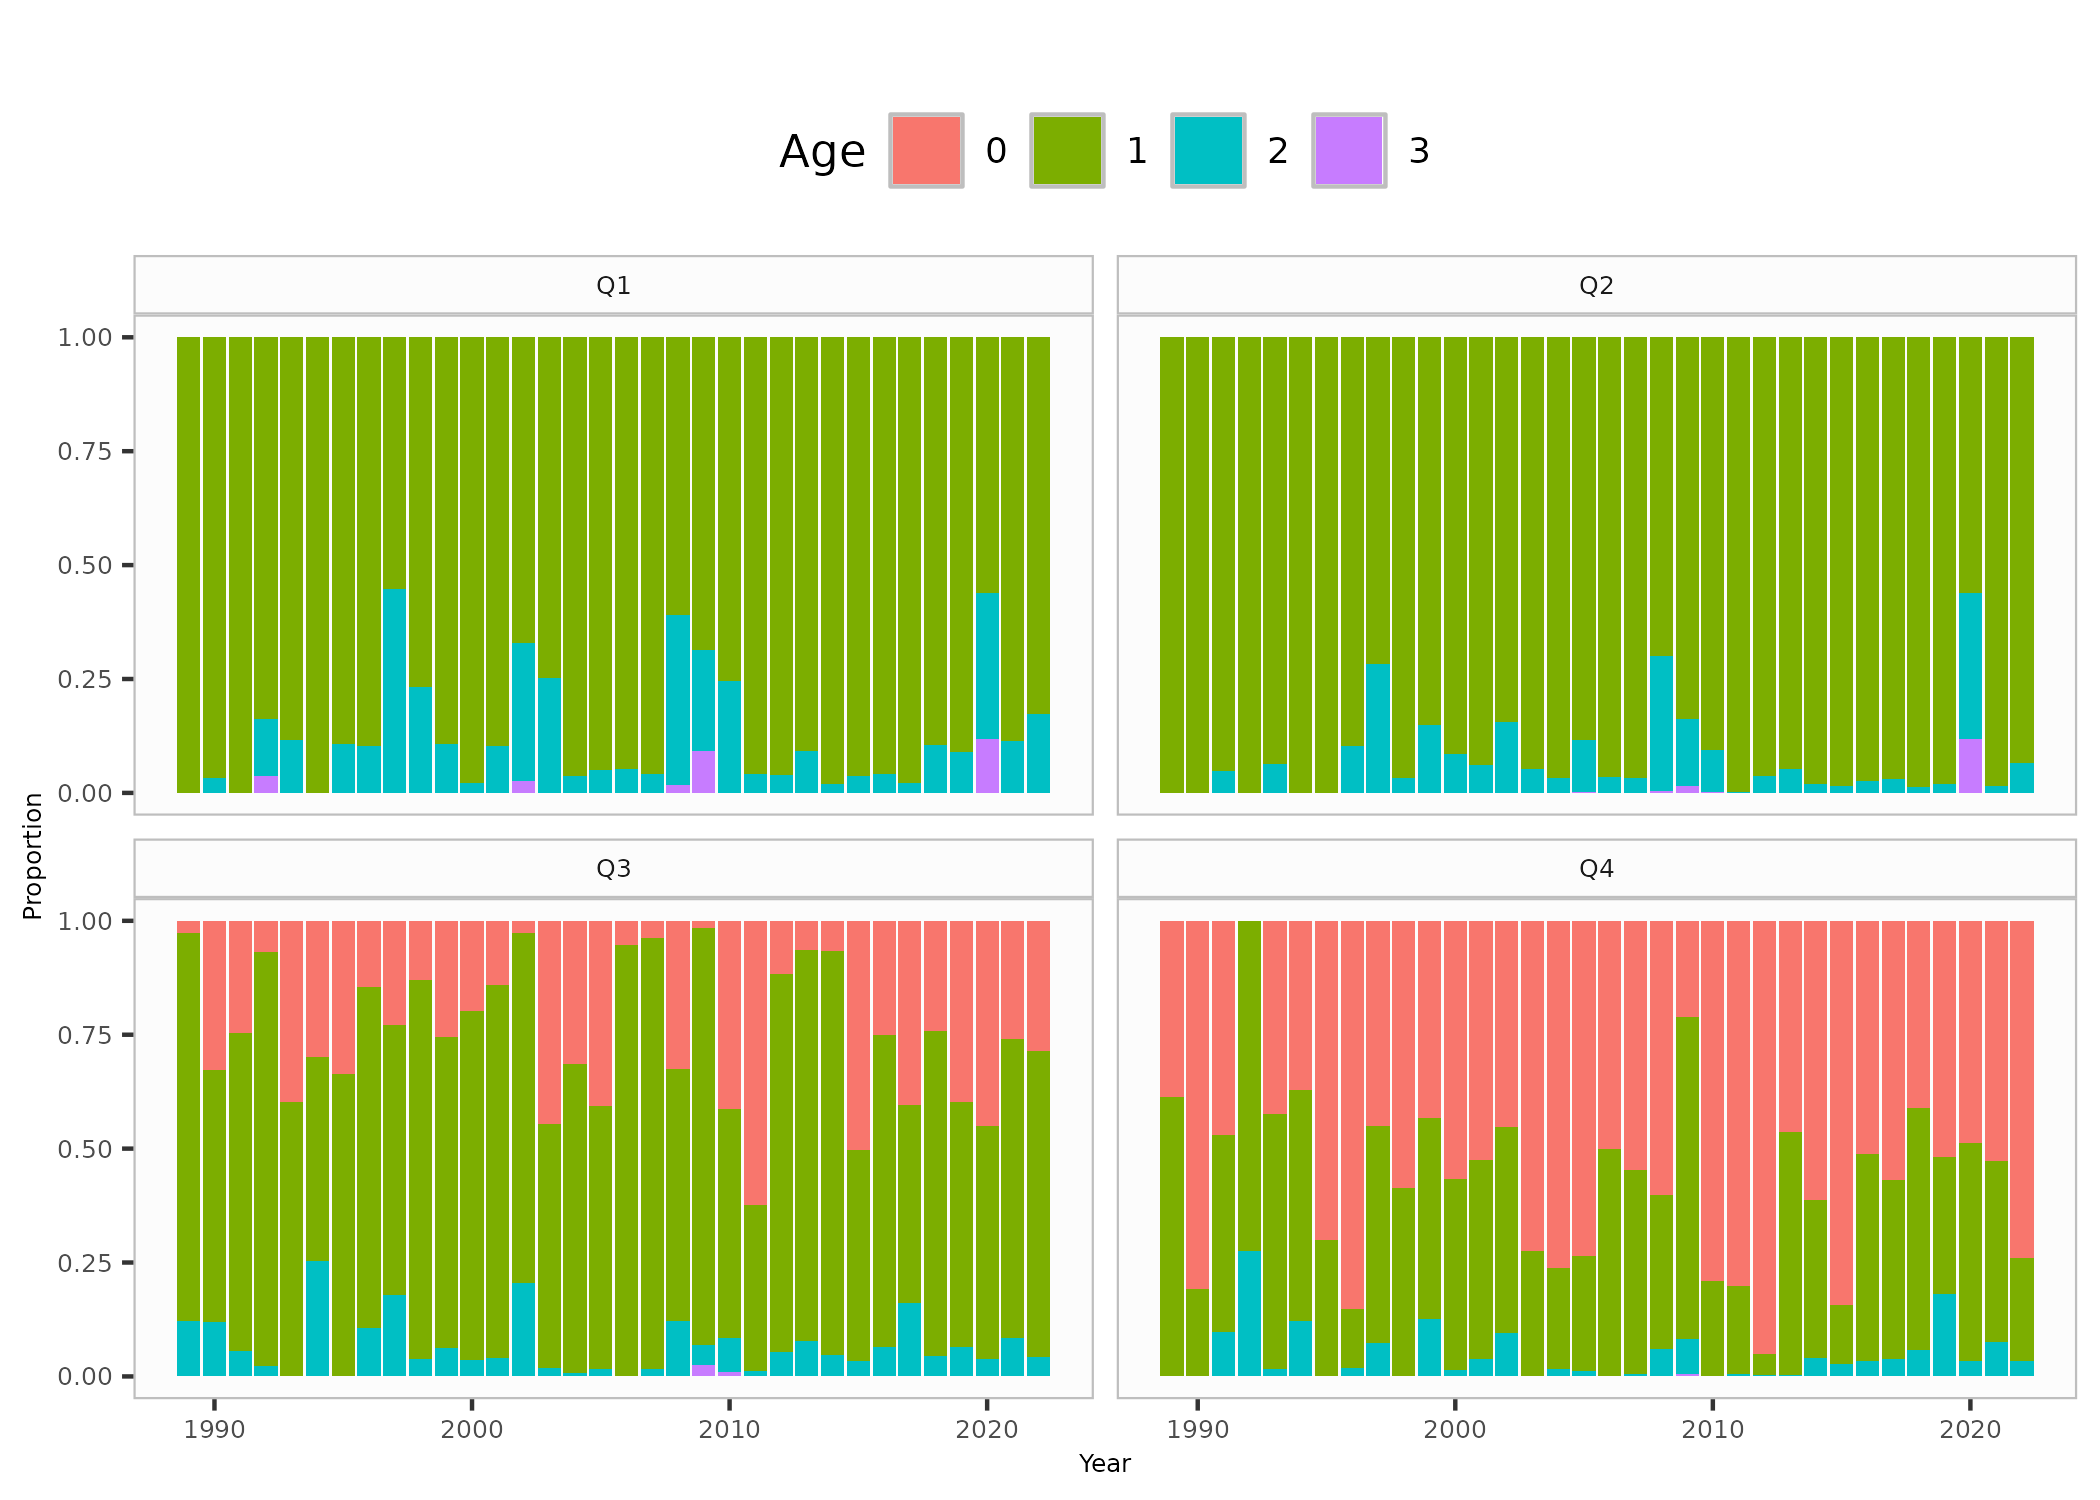
\includegraphics[width=0.95\linewidth]{report/run/S1.0_4FLEETS/fig_agecomp_by_quartersSeine} 

}

\caption{ane.27.9a stock. Age proportion of the commercial fleet (*SEINE*) by quarter (1989 to 2023).}\label{fig:unnamed-chunk-7}
\end{figure}

Figure 7 shows the yearly age proportions from surveys \emph{PELAGO},
\emph{ECOCADIZ}, and \emph{ECOCADIZ-RECLUTAS} that were used as input
for the model. It can be observed that in the \emph{PELAGO} survey,
conducted in the second quarter (Q2), age 1 represents the highest
proportion over time, with a presence of ages 2 and 3, and no records of
age 0 individuals. The \emph{ECOCADIZ} survey, primarily conducted in
the third quarter (Q3), shows a predominance of age 1, with an increase
in the proportion of age 0 from 2010 onward; in 2004 and 2006, when the
survey was conducted in the second quarter (Q2), no age 0 individuals
were recorded by convention. The \emph{ECOCADIZ-RECLUTAS} survey,
conducted since 2014 in October (fourth quarter, Q4), shows a higher
proportion of age 0, followed by age 1, with lower representation of
ages 2 and 3.

\begin{figure}[H]

{\centering 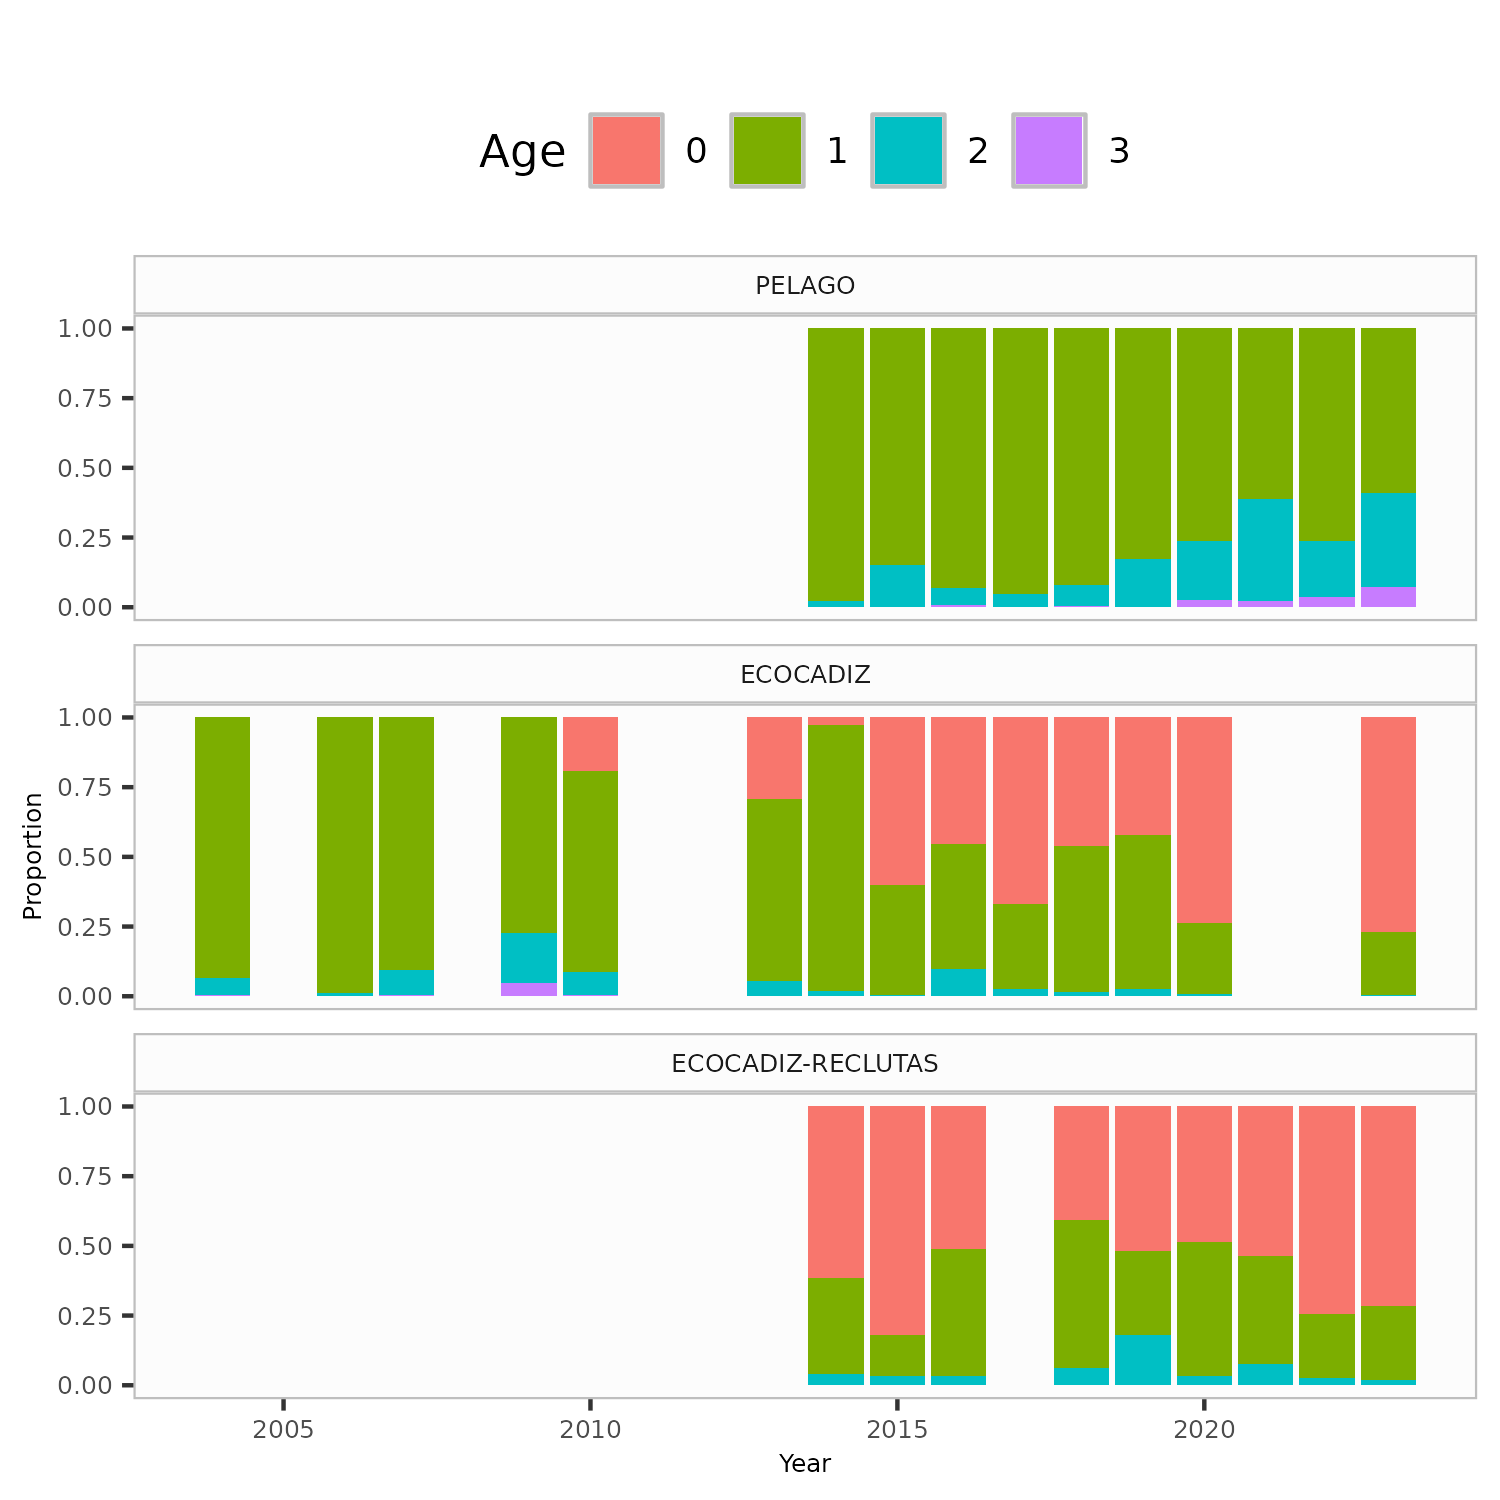
\includegraphics[width=0.95\linewidth]{report/run/S1.0_4FLEETS/fig_agecomp_by_quartersSurveys} 

}

\caption{ane.27.9a stock. Age proportion by surveys  (*PELAGO*, *ECOCADIZ*, and *ECOCADIZ-RECLUTAS*).}\label{fig:unnamed-chunk-8}
\end{figure}

\hypertarget{weigth-at-age}{%
\subsection{Weigth-at-age}\label{weigth-at-age}}

Figure 8 presents the age-specific weight-at-age values at the start of
each season, estimated from external data sources. The figure
illustrates that mean weight differences between age groups remain
consistent over time, with some variability observed across quarters.
Individuals aged 3 show greater variability in mean weight compared to
younger age groups. For further details, refer to the working document
by \textbf{Zuñiga et al.~(2024)}.

\begin{figure}[H]

{\centering 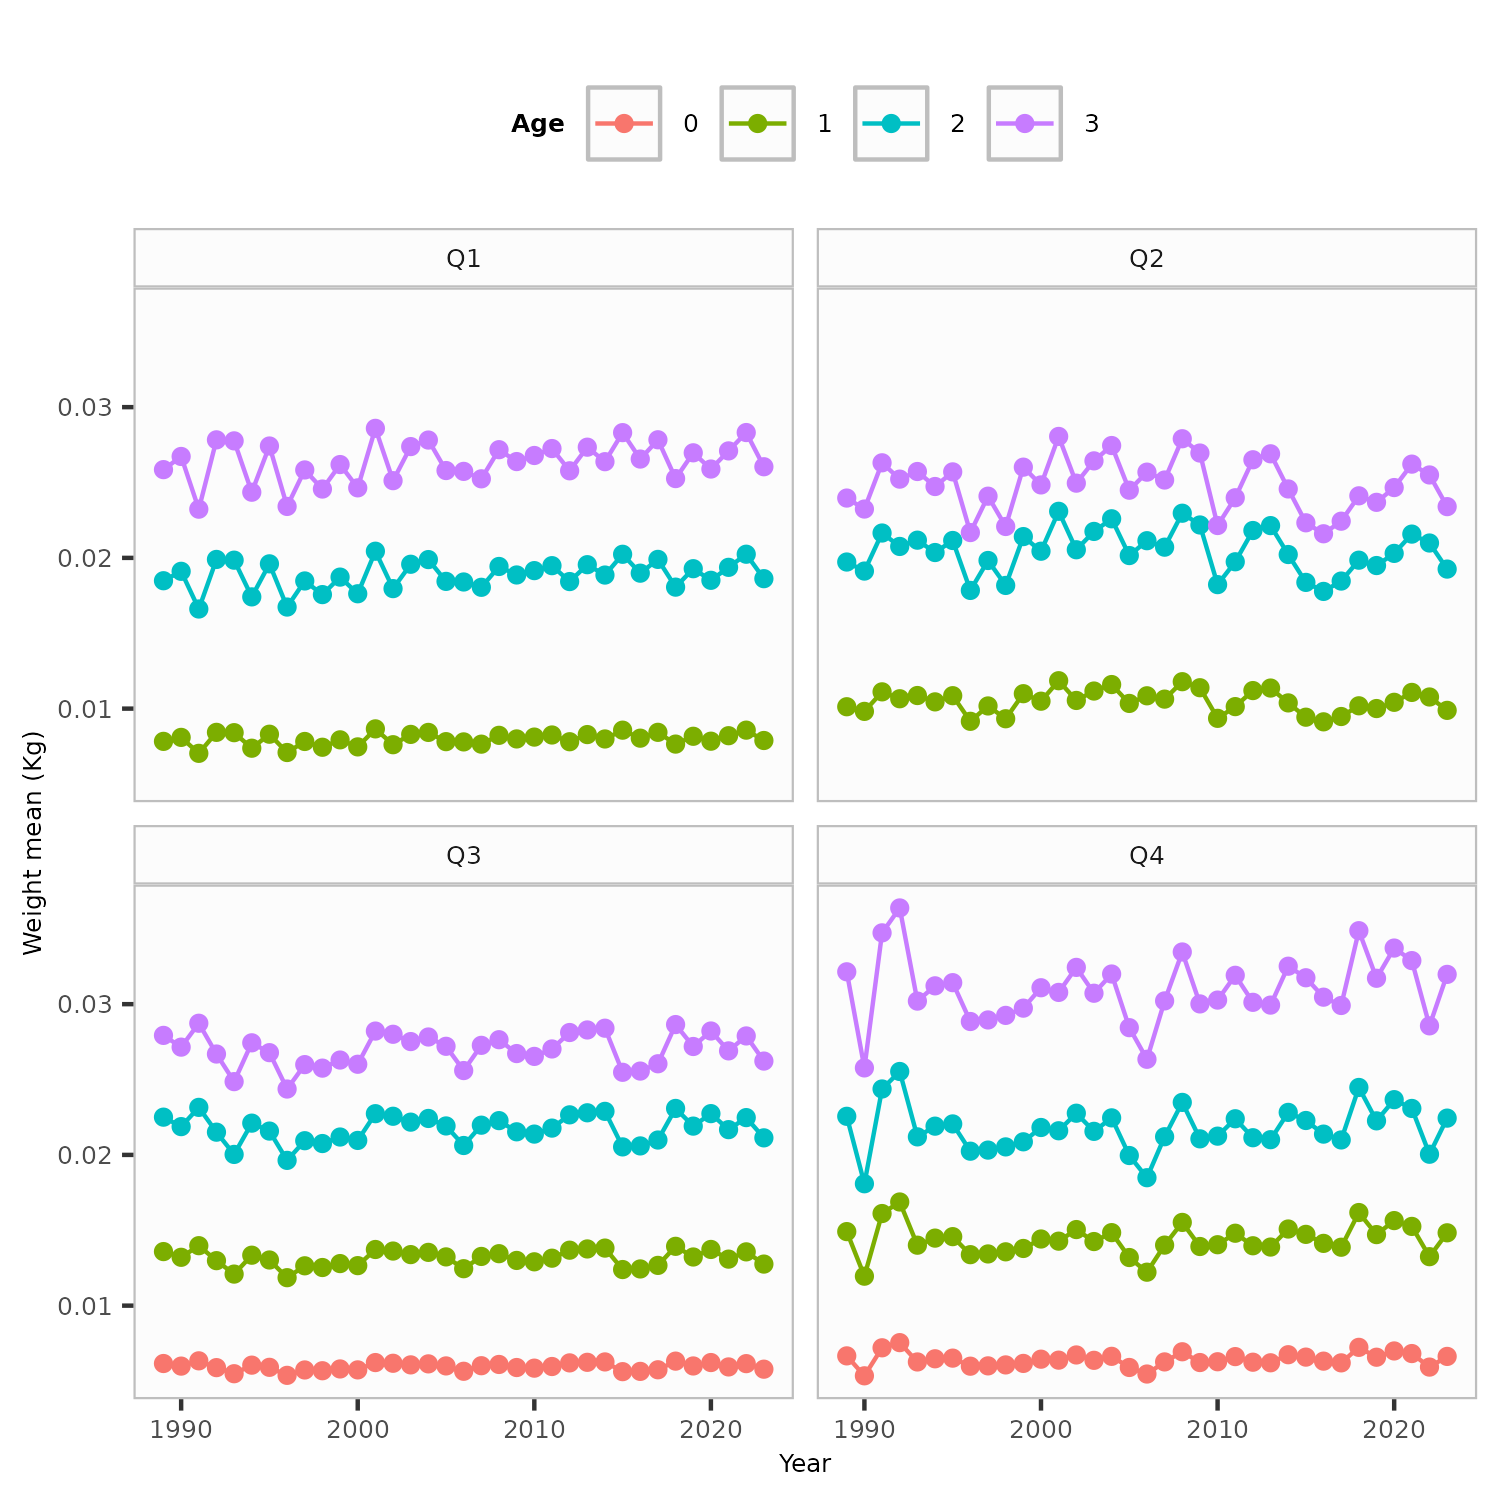
\includegraphics[width=0.95\linewidth]{report/run/S1.0_4FLEETS/fig_weight_by_quarters} 

}

\caption{ane.27.9a stock. Weight at age by quarters.}\label{fig:unnamed-chunk-9}
\end{figure}

\hypertarget{model-settings}{%
\subsection{Model settings}\label{model-settings}}

\hypertarget{natural-mortality}{%
\subsubsection{Natural mortality}\label{natural-mortality}}

Age-specific natural mortality input values at the beginning of the
year, which were derived from external data sources. For further
details, refer to the working document by \textbf{Rincón et al.~(2024)}.

\begin{center}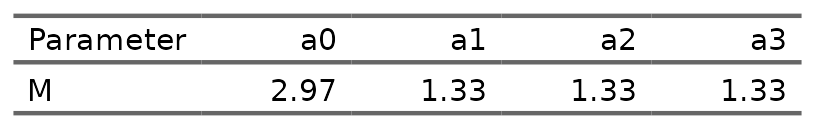
\includegraphics[width=0.95\linewidth]{report/run/S1.0_4FLEETS/tb_natM} \end{center}

\hypertarget{maturity}{%
\subsubsection{Maturity}\label{maturity}}

Due to some inconsistencies in the maturity ogives not noticed during
WKPELA 2018, we assume that all individuals with age 1 or higher (B1+),
are mature i.e.~these abundance estimates result equivalent to spawning
stock biomass estimates. For further details, refer to the working
document by \textbf{ICES 2024 and WD Rincón et al.~(2024)}.

\begin{center}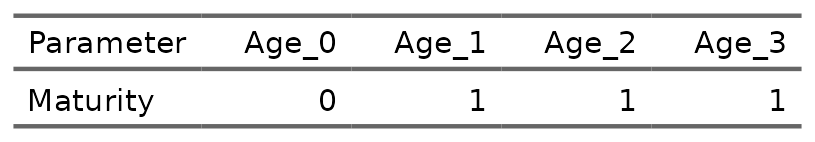
\includegraphics[width=0.95\linewidth]{report/run/S1.0_4FLEETS/tb_maturity} \end{center}

\hypertarget{growth}{%
\subsubsection{Growth}\label{growth}}

It is not modelled explicitly.

\hypertarget{recruitment}{%
\subsubsection{Recruitment}\label{recruitment}}

Equilibrium recruitment (\(R_0\)) was estimated in the base model, and
steepness (h) was fixed at 0.8. The initial steepness estimate is based
on values reported by Hsu \emph{et al.} (2024) , with a mean of 0.82 and
a range of 0.59 to 0.93, and by Wiff \emph{et al.} (2018), who reported
steepness values between 0.58 and 0.86 for pelagic species. Standard
deviation of log number of recruits was set to 0.6.

The early recruitment deviations for the initial population were
estimated for the period 1985-1988. A recruitment bias adjustment ramp
(Methot and Taylor, 2011) was applied to this early period, and
bias-adjusted recruitment was estimated for the main period. Recruitment
deviations for the main period were estimated for 1991-2023.

\hypertarget{fishing-mortality}{%
\subsubsection{Fishing mortality}\label{fishing-mortality}}

Calculation of fishing mortality is performed by using the hybrid F
method that does a Pope's approximation to provide initial values for
iterative adjustment of the Baranov continuous F values to closely
approximate the observed catch.Total catch biomass by year is assumed to
be accurate and precise and the F values are tuned to match this catch.

\hypertarget{catchability}{%
\subsubsection{Catchability}\label{catchability}}

All the surveys are assumed to be relative indices of abundance. The
catchability are modelled with a simple \(q\) linear model.

\hypertarget{selectivity}{%
\subsubsection{Selectivity}\label{selectivity}}

The fishery and the surveys selectivity were defined as logistic
functions fixed over time.

\hypertarget{data-weighting}{%
\subsubsection{Data weighting}\label{data-weighting}}

Constant standard errors of 0.05 and 0.3 were assumed for quarterly
catches and surveys, respectively.

The age composition were adjusted assuming a multinomial error structure
with variance described by the sample size, set at 100 for both, the
commercial fleet and acoustic surveys. After that, these data was
weighted using the Francis method TA1.8 (Francis, 2011).

\hypertarget{initial-population}{%
\subsubsection{Initial population}\label{initial-population}}

It is calculated by estimating an initial equilibrium population
modified by age composition data in the first year of the assessment
(Methot and Wetzel, 2013). The model starts in 1989 and the equilibrium
population age structure was assumed to be in an exploited state with an
initial catch of 0 tonnes

A summary of the model key model assumptions and parameters for the
Stock Synthesis is available in Figure 9.

\begin{figure}[H]

{\centering 
\includegraphics[width=0.95\linewidth]{report/run/S1.0_4FLEETS/tb_dat_stru} 

}

\caption{ane.27.9a stock. Input data type, model assumptions and settings for the assessment  with data series 1989-2023.}\label{fig:unnamed-chunk-12}
\end{figure}

Variance estimates for all estimated parameters are calculated from the
Hessian matrix. Minimisation of the likelihood is implemented in phases
using standard ADMB process. The phases in which estimation will begin
for each parameter is shown in the control file available in the TAF
repository for this stock . The R packages r4ss version 1.50.0 (Taylor
\emph{et al.}, 2021) and ss3diags version 1.10.2 (Carvalho \emph{et
al.}, 2021) were used to process and view model outputs. All analyses
were conduction in R version 4.4.1 (2024-06-14).

\hypertarget{diagnostics}{%
\section{Diagnostics}\label{diagnostics}}

The model successfully converged, as evidenced by the Hessian matrix
being positive definite and the final gradient being relatively small,
with a gradient value of 0.0000556. The ``Status'' column in Figure 10
shows that the initial model configuration has allowed for adequate
optimization of the parameters. Additionally, the gradient for all
parameters is relatively small. It is important to note that the bounds
imposed on the initial parameters have not restricted the search for
optimized values, as reflected in the ``Afterbound'' column.

\begin{figure}[H]

{\centering 
\includegraphics[width=0.95\linewidth]{report/run/S1.0_4FLEETS/tb_params_est} 

}

\caption{ane.27.9a stock. Parameters estimated by the initial base model.}\label{fig:unnamed-chunk-13}
\end{figure}

\hypertarget{model-fit-and-residuals}{%
\subsection{Model fit and residuals}\label{model-fit-and-residuals}}

The Figure 11 shows that the abundance indices from the acoustic surveys
exhibit a high level of variability, as reflected by the width of the
assumed confidence intervals, with a maximum coefficient of variation of
30\%. The model follows the overall trend of the indices, though it
encounters some difficulties in accurately fitting the extreme biomass
values, both the highest and lowest. However, it adequately reproduces
the general trend of variability in biomass levels presented by the
survey estimates.

\begin{figure}[H]

{\centering 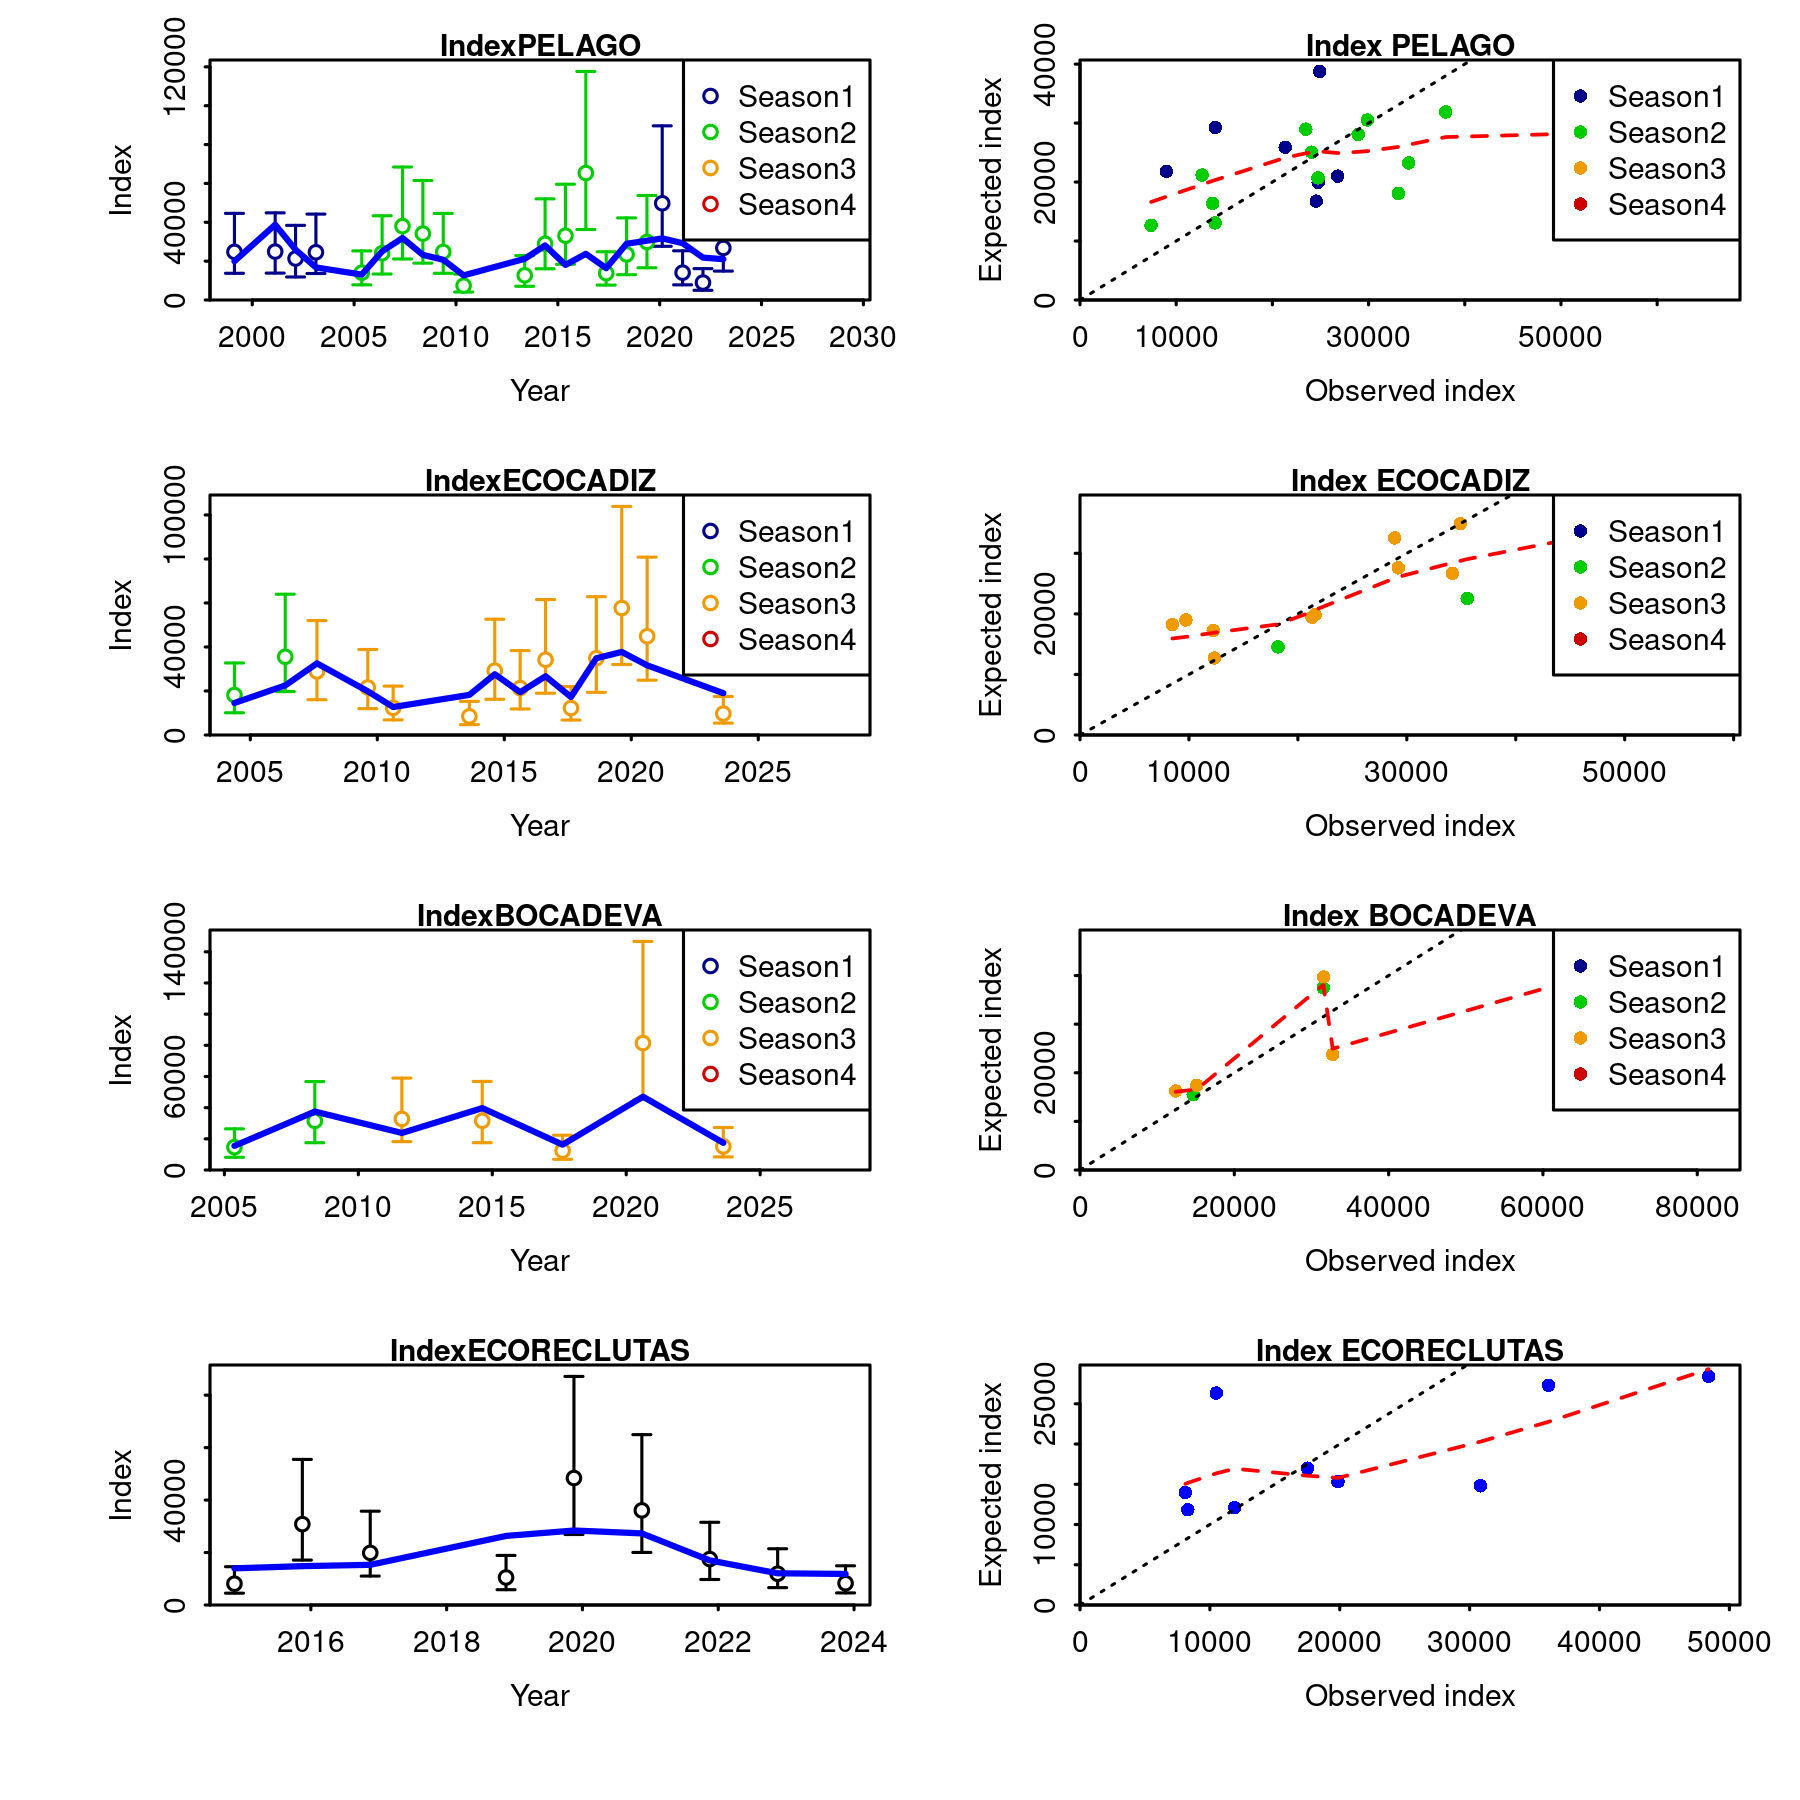
\includegraphics[width=0.95\linewidth]{report/run/S1.0_4FLEETS/fig_indices_fit} 

}

\caption{ane.27.9a stock. Model fit to the data (left panel) and observed versus expected values (right panel) of the indices from the surveys *PELAGO*, *ECOCADIZ*, *BOCADEVA* and *ECOCADIZ-RECLUTAS*. The lines indicate a 95\% uncertainty interval around the index values based on the lognormal error model assumption. }\label{fig:unnamed-chunk-14}
\end{figure}

Figure 12 shows that the residuals from the fit of the biomass indices
are randomly distributed, with p-values greater than 0.05 (\emph{PELAGO}
= 0.415, \emph{ECOCADIZ} = 0.636, \emph{BOCADEVA} = 0.888,
\emph{ECOCADIZ-RECLUTAS} = 0.374). The estimated root mean square error
(RMSE) for the joint residual analysis is 41.7\%.

\begin{figure}[H]

{\centering 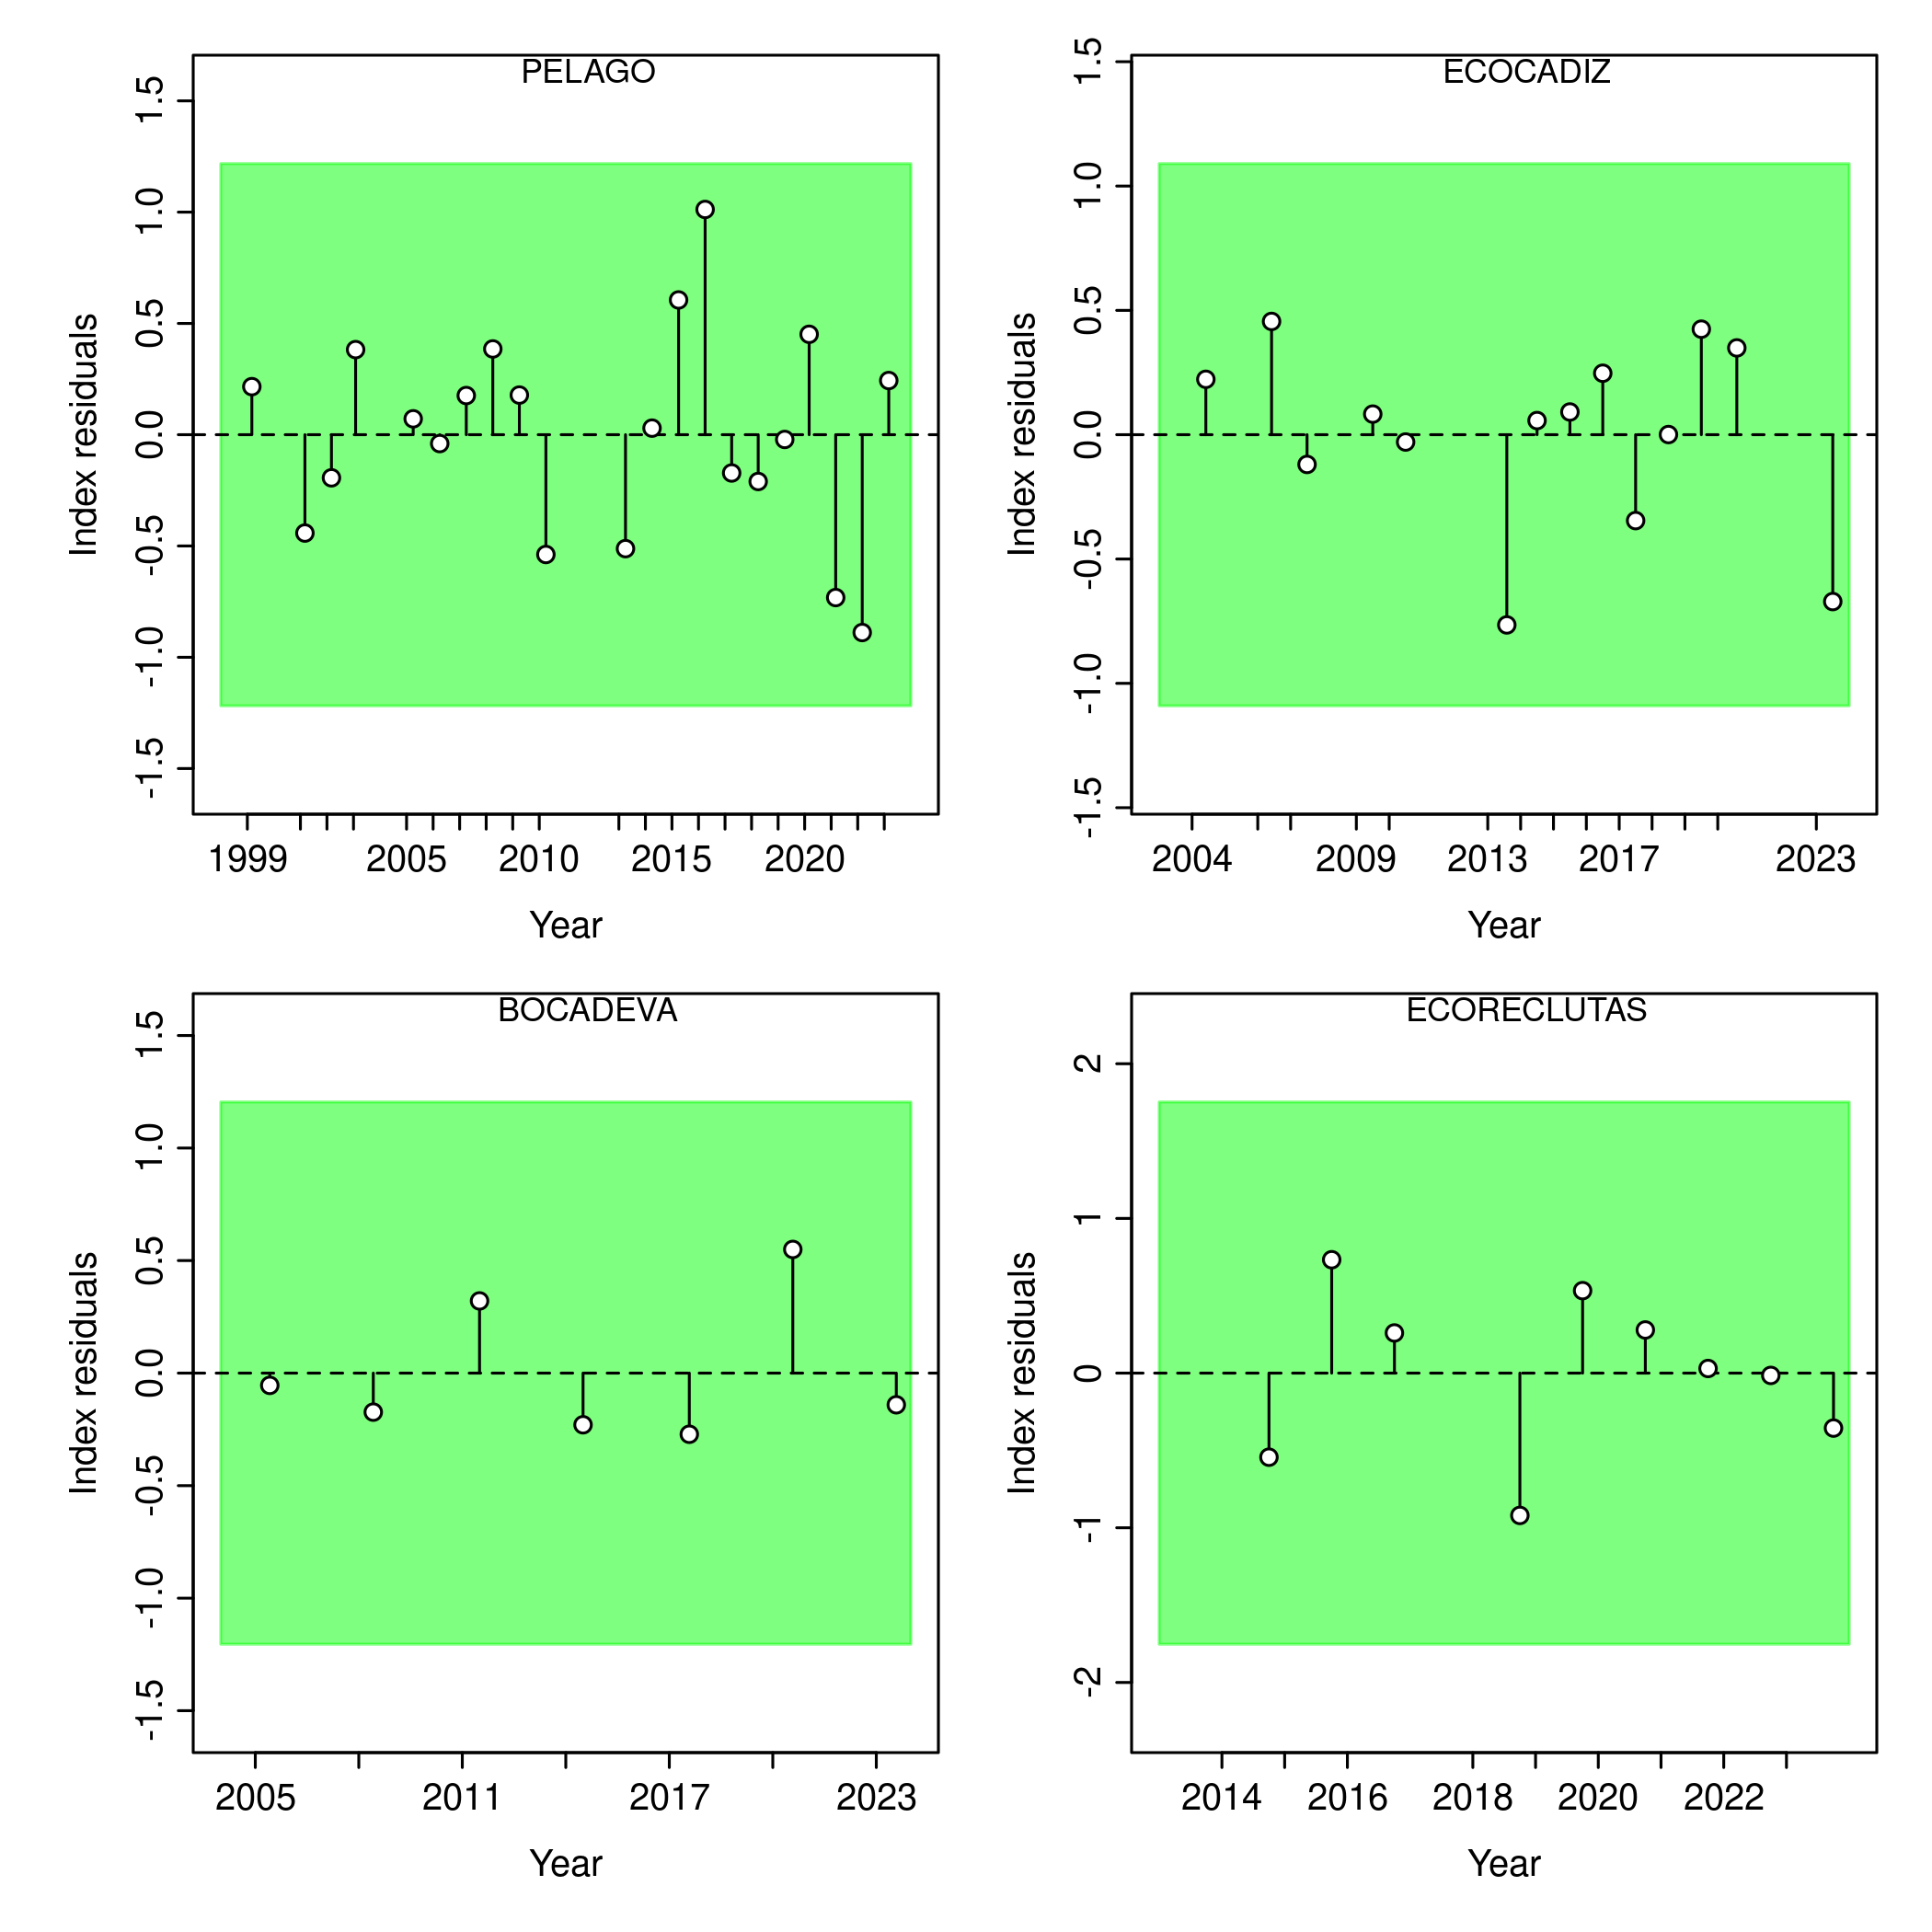
\includegraphics[width=0.95\linewidth]{report/run/S1.0_4FLEETS/fig_runtest_residuals_indices} 

}

\caption{ane.27.9a stock. a) Run test plots for the fit of acoustic survey indices. Green shading indicates no evidence (p>=0.05) and red shading indicates evidence (p<0.05) for rejecting the hypothesis of a randomly distributed residual time series, respectively. The shaded area (green/red) spans three standard residual deviations on either side of zero, and red points outside the shading violate the three-sigma limit for that series. b) Joint residual plots for the fit of acoustic survey indices (bottom left panel).  Vertical lines with points show the residuals, and the solid black line show loess smoother through all residuals. Boxplots indicate the median and quantiles in cases where residuals from multiple indices are available for a given year, with the solid black line showing a loess smoother. The root mean square error (RMSE) is included in the top right corner of the panel.}\label{fig:unnamed-chunk-15}
\end{figure}

In the case of the commercial fleet (\emph{SEINE}), the model captures
the observed fluctuations in the mean age, remaining around 1 year. For
the \emph{PELAGO} survey, the model follows the oscillation in the mean
age, adjusting between 1 and 1.4 years, though it encounters some
fitting issues in the later years of the series. In \emph{ECOCADIZ}, the
observed trend shows a progressive decline in mean age, starting near
1.0 and dropping below 0.5 in recent years, with the model struggling to
fit this trend. Finally, in \emph{ECOCADIZ-RECLUTAS}, the model fits
well to an initial mean age below 0.5 years, increasing above 0.5
between 2016 and 2021, before decreasing again in the last two years of
the series.

\begin{figure}[H]

{\centering 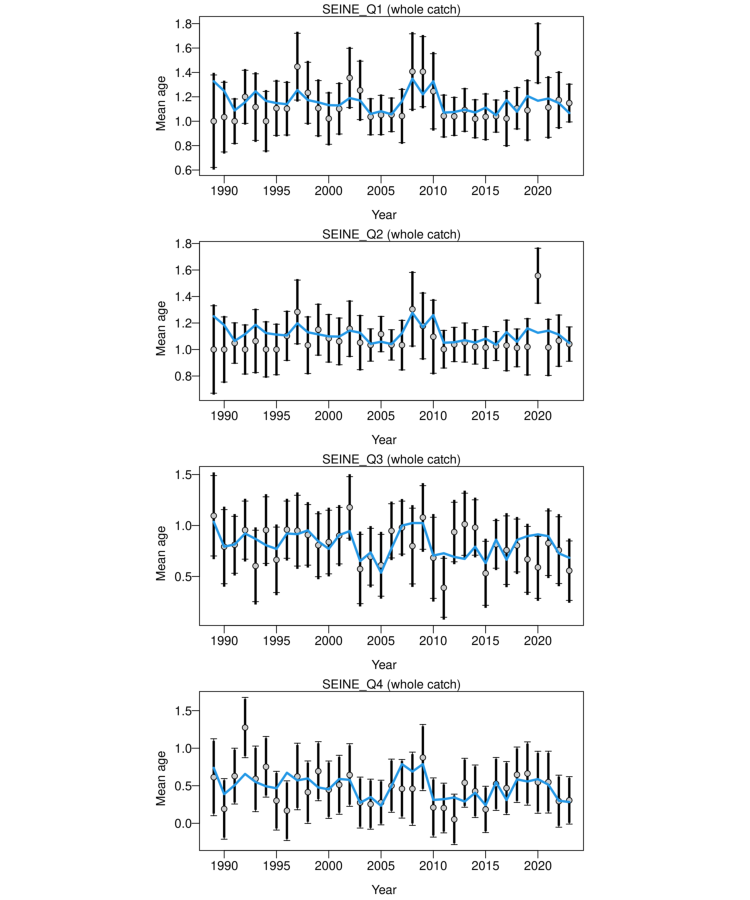
\includegraphics[width=0.95\linewidth]{Report_SS3_quarter_with_age_data_S1.0_4FLEETS_files/figure-latex/unnamed-chunk-16-1} 

}

\caption{Mean age for commercial fleet by quarters with 95\% confidence intervals based on current sample sizes. Francis data weighting method TA1.8: thinner intervals (with capped ends) show the result of further adjusting sample sizes based on the suggested multiplier (with 95\% interval) for age data. The blue line corresponds to the estimated mean age.}\label{fig:unnamed-chunk-16}
\end{figure}

\begin{figure}[H]

{\centering 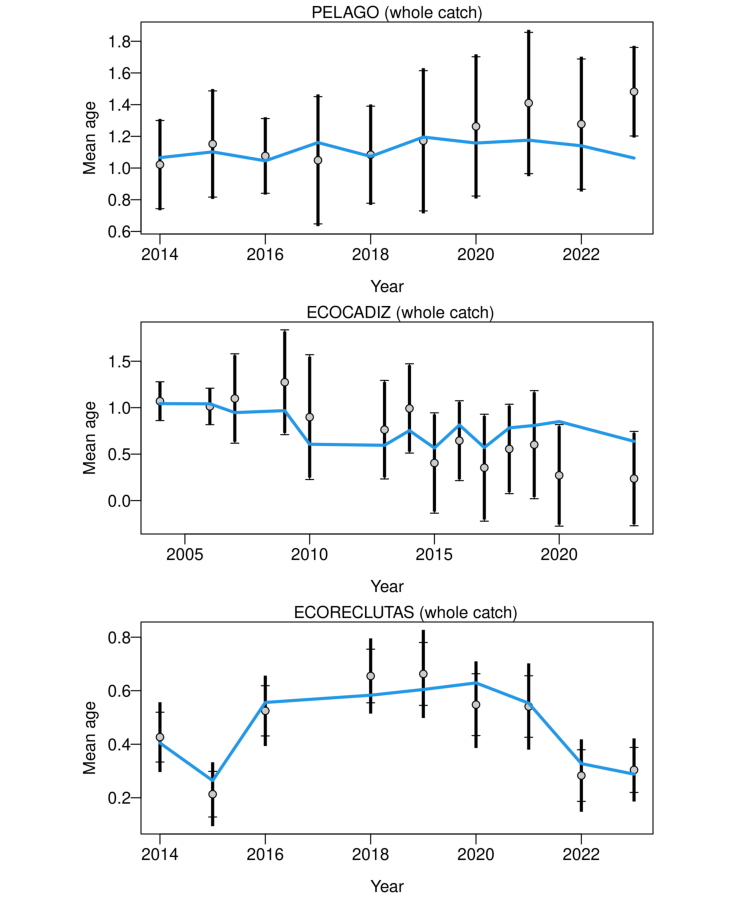
\includegraphics[width=0.95\linewidth]{Report_SS3_quarter_with_age_data_S1.0_4FLEETS_files/figure-latex/unnamed-chunk-17-1} 

}

\caption{Mean age for *PELAGO*, *ECOCADIZ*, and *ECOCADIZ-RECLUTAS* with 95\% confidence intervals based on current sample sizes. Francis data weighting method TA1.8: thinner intervals (with capped ends) show the result of further adjusting sample sizes based on the suggested multiplier (with 95\% interval) for age data. The blue line corresponds to the estimated mean age.}\label{fig:unnamed-chunk-17}
\end{figure}

The Figure 13 shows the aggregated age compositions over time for the
different age data sources: \emph{SEINE}, \emph{ECOCADIZ},
\emph{PELAGO}, and \emph{ECORECLUTAS}. Overall, a high proportion of
young individuals (ages 0 and 1) is observed in both the commercial
fleet catches and acoustic surveys, with a significant decline in the
proportions of older age classes. The green lines represent the model
fits, demonstrating an adequate fit, with the aggregated age
compositions well reconstructed.

\begin{figure}[H]

{\centering 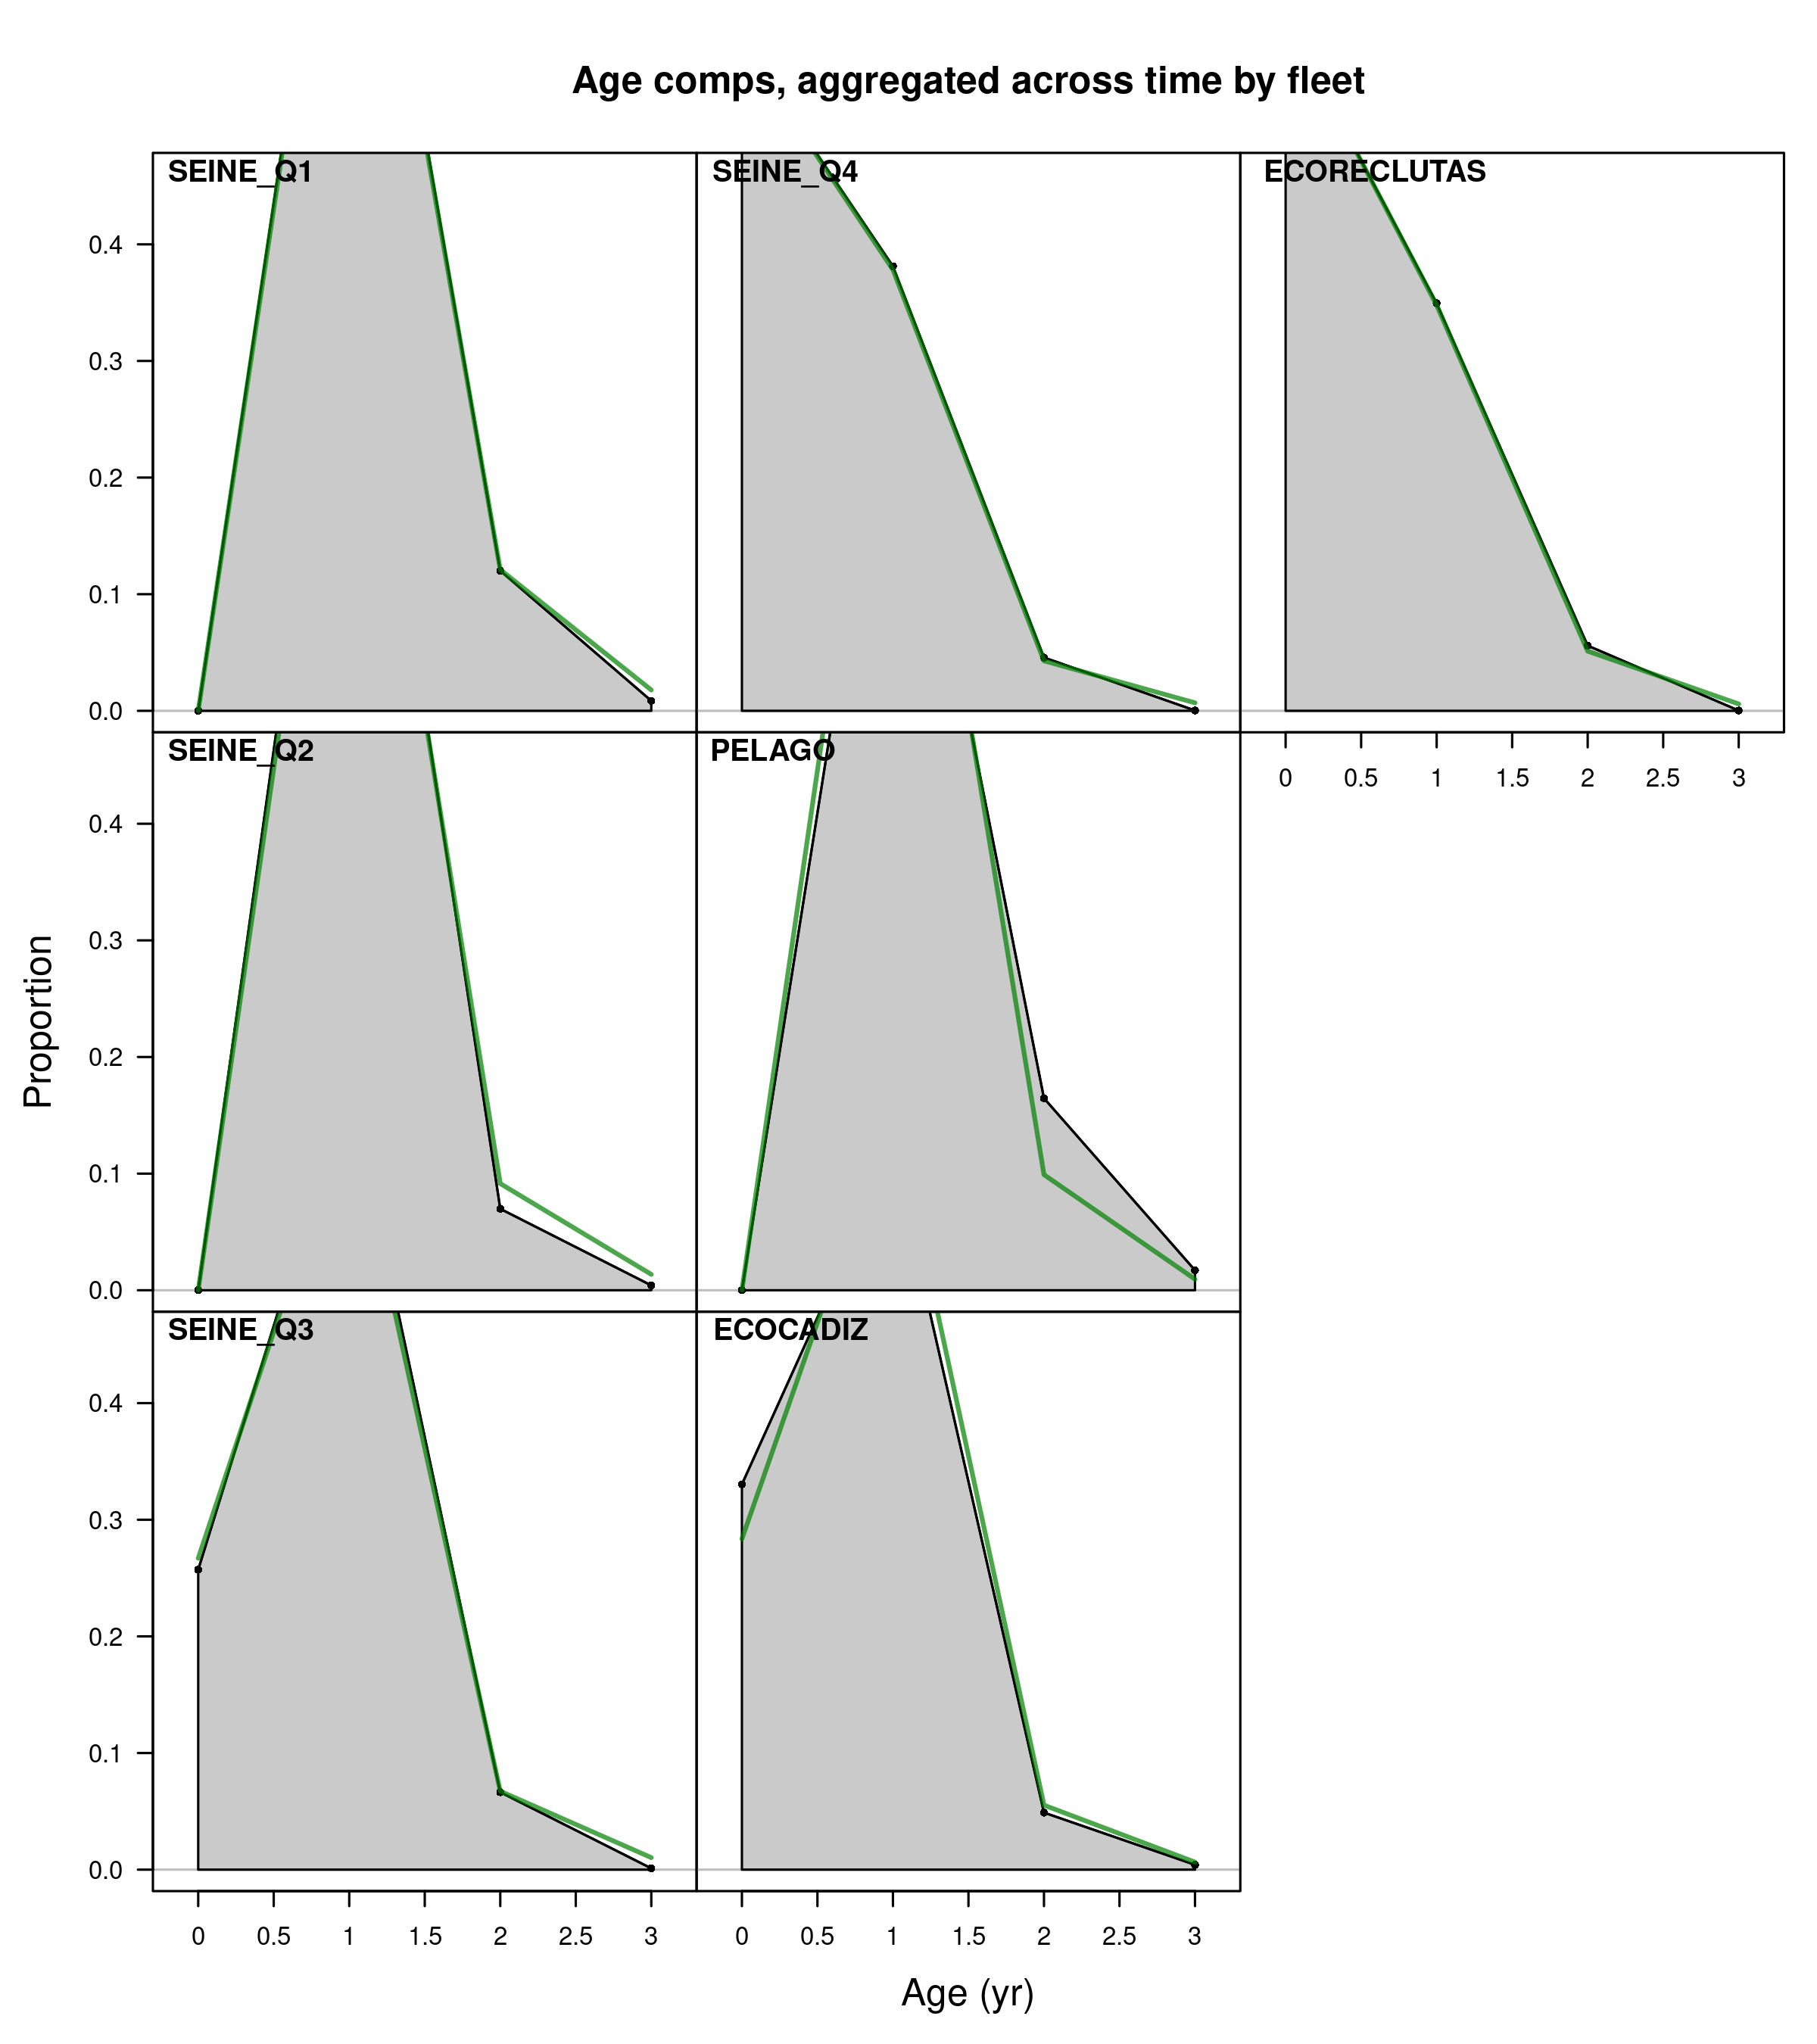
\includegraphics[width=0.95\linewidth]{report/run/S1.0_4FLEETS/fig_age_fit_agg} 

}

\caption{ane.27.9a stock. Model fit to the aggregated age composition data from the SEINE fishery, and the acoustic surveys *PELAGO*, *ECOCADIZ*, and *ECOCADIZ-RECLUTAS*. The green line represents the model estimates, while the shaded grey area shows the observed data.}\label{fig:unnamed-chunk-18}
\end{figure}

Although the aggregated fits show an overall adequate result, some years
exhibit variability in the age composition of the commercial fleet
(SEINE) catches, leading to reduced precision in the fits for the fourth
quarter, particularly in 1991, 1996, and 2012 (Figure 14). This pattern
is also evident in the annual data fits for the PELAGO survey,
especially in the later years of the series (2020-2023), where there is
a tendency to overestimate age 1 and underestimate age 2 (Figure 14). In
the ECOCADIZ survey, there are difficulties in estimating ages 0 and 1,
with a tendency to underestimate age 0 and overestimate age 1 from 2016
to 2023 (Figure 14). In ECOCADIZ-RECLUTAS, a generally good fit is
observed without a clear pattern of overestimation or underestimation
(Figure 14). These patterns are also reflected in the bubble plots of
the residuals corresponding to the fit of these data (Figure 14).

\begin{figure}[H]

{\centering 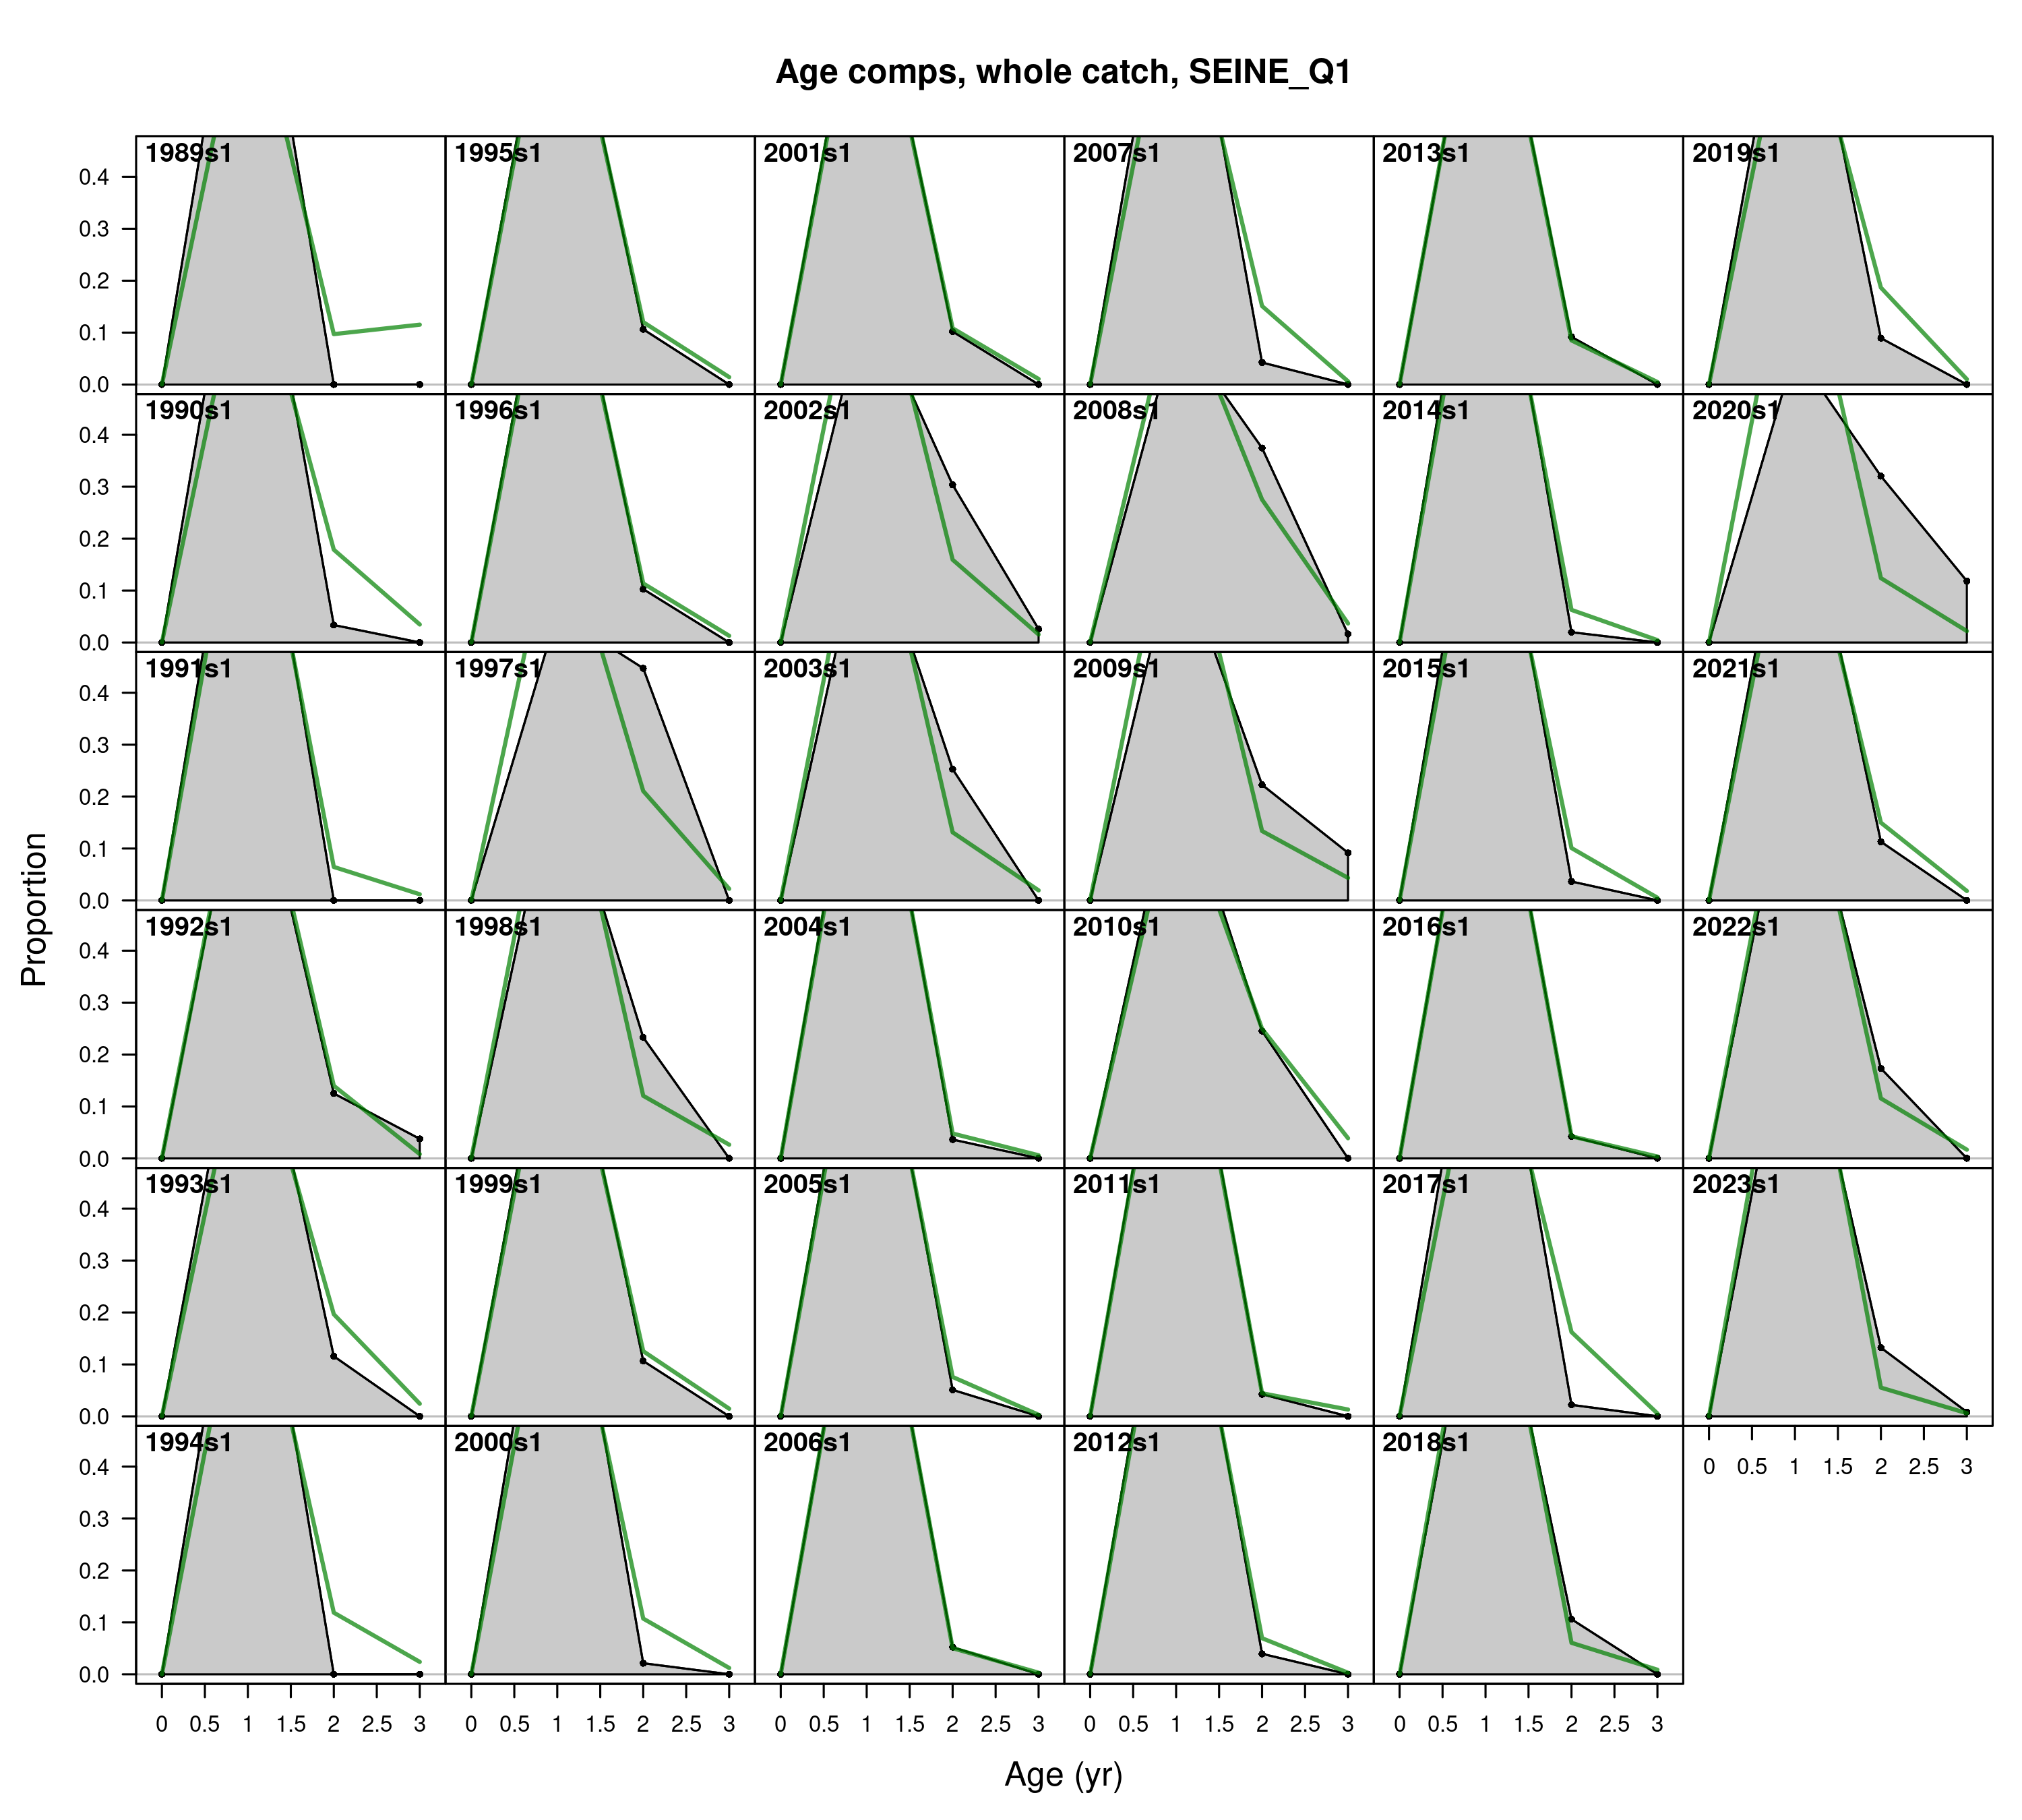
\includegraphics[width=0.95\linewidth]{report/run/S1.0_4FLEETS/fig_age_fit_SeineQ1} 

}

\caption{ane.27.9a stock. Model fit to the age composition data from the *SEINEQ1* fishery, by year and quarter. The green line represents the model estimates, while the shaded grey area shows the observed data.}\label{fig:unnamed-chunk-19}
\end{figure}

\begin{figure}[H]

{\centering 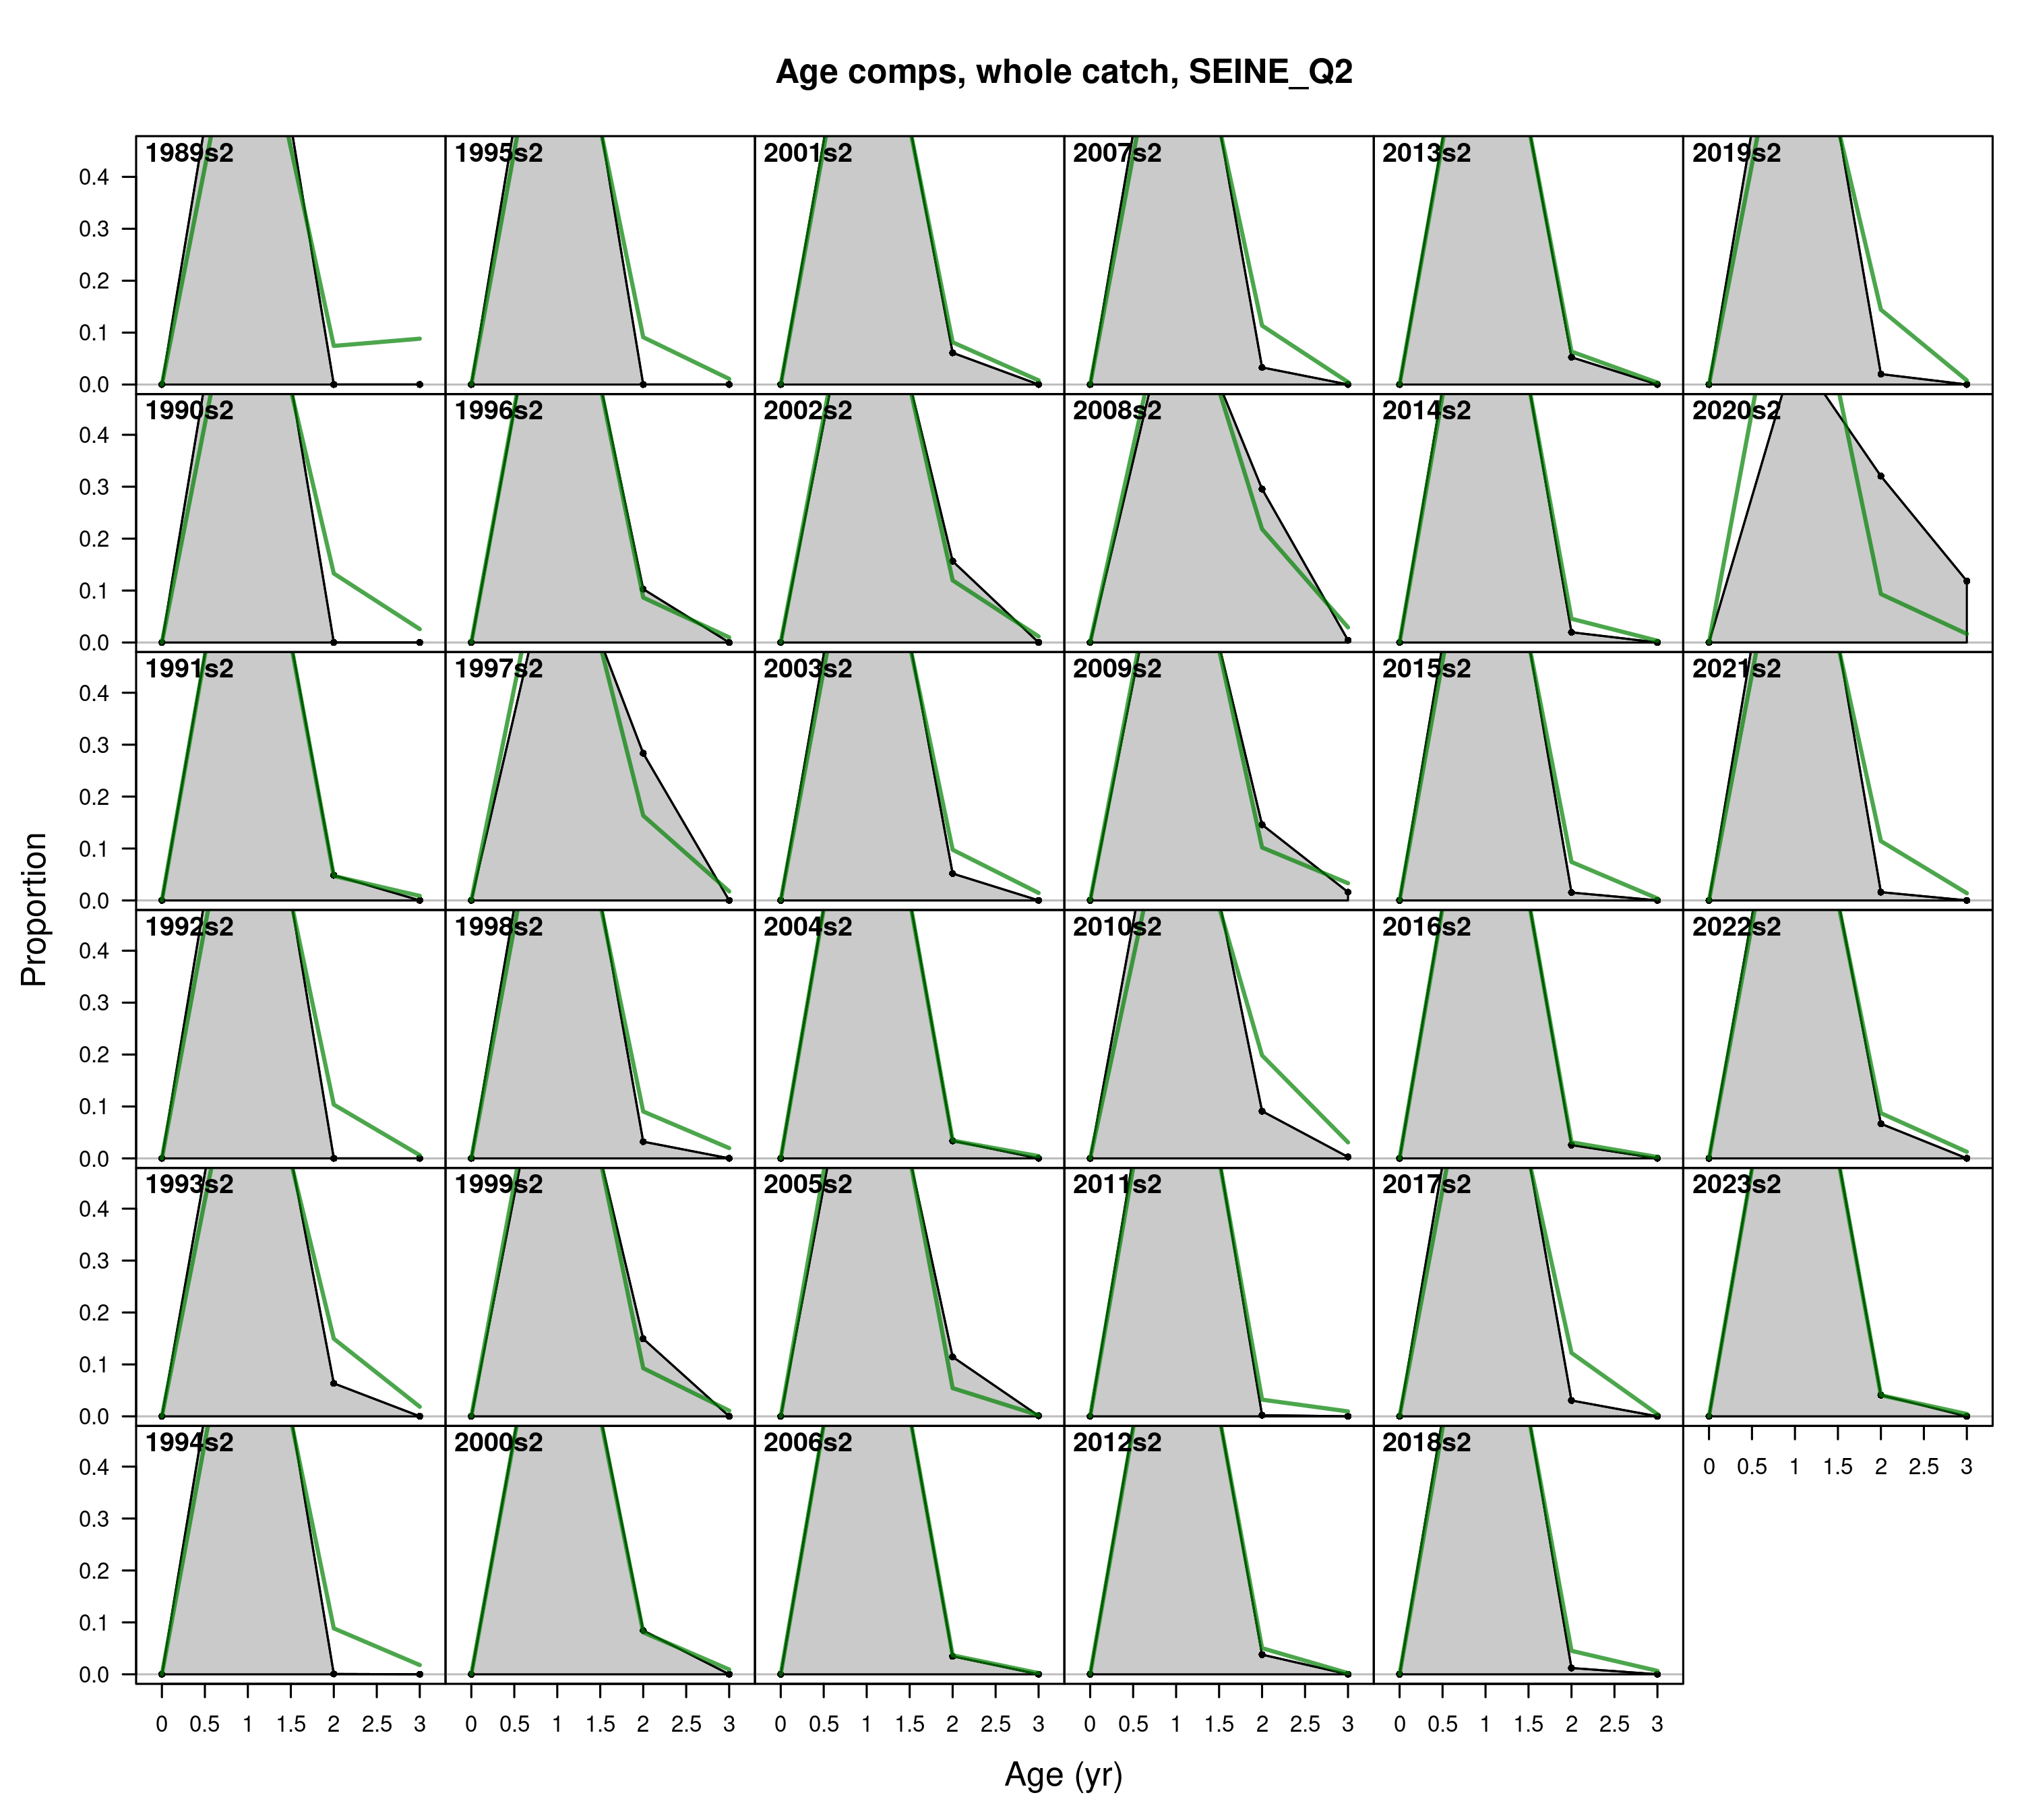
\includegraphics[width=0.95\linewidth]{report/run/S1.0_4FLEETS/fig_age_fit_SeineQ2} 

}

\caption{ane.27.9a stock. Model fit to the age composition data from the *SEINEQ2* fishery, by year and quarter. The green line represents the model estimates, while the shaded grey area shows the observed data.}\label{fig:unnamed-chunk-20}
\end{figure}

\begin{figure}[H]

{\centering 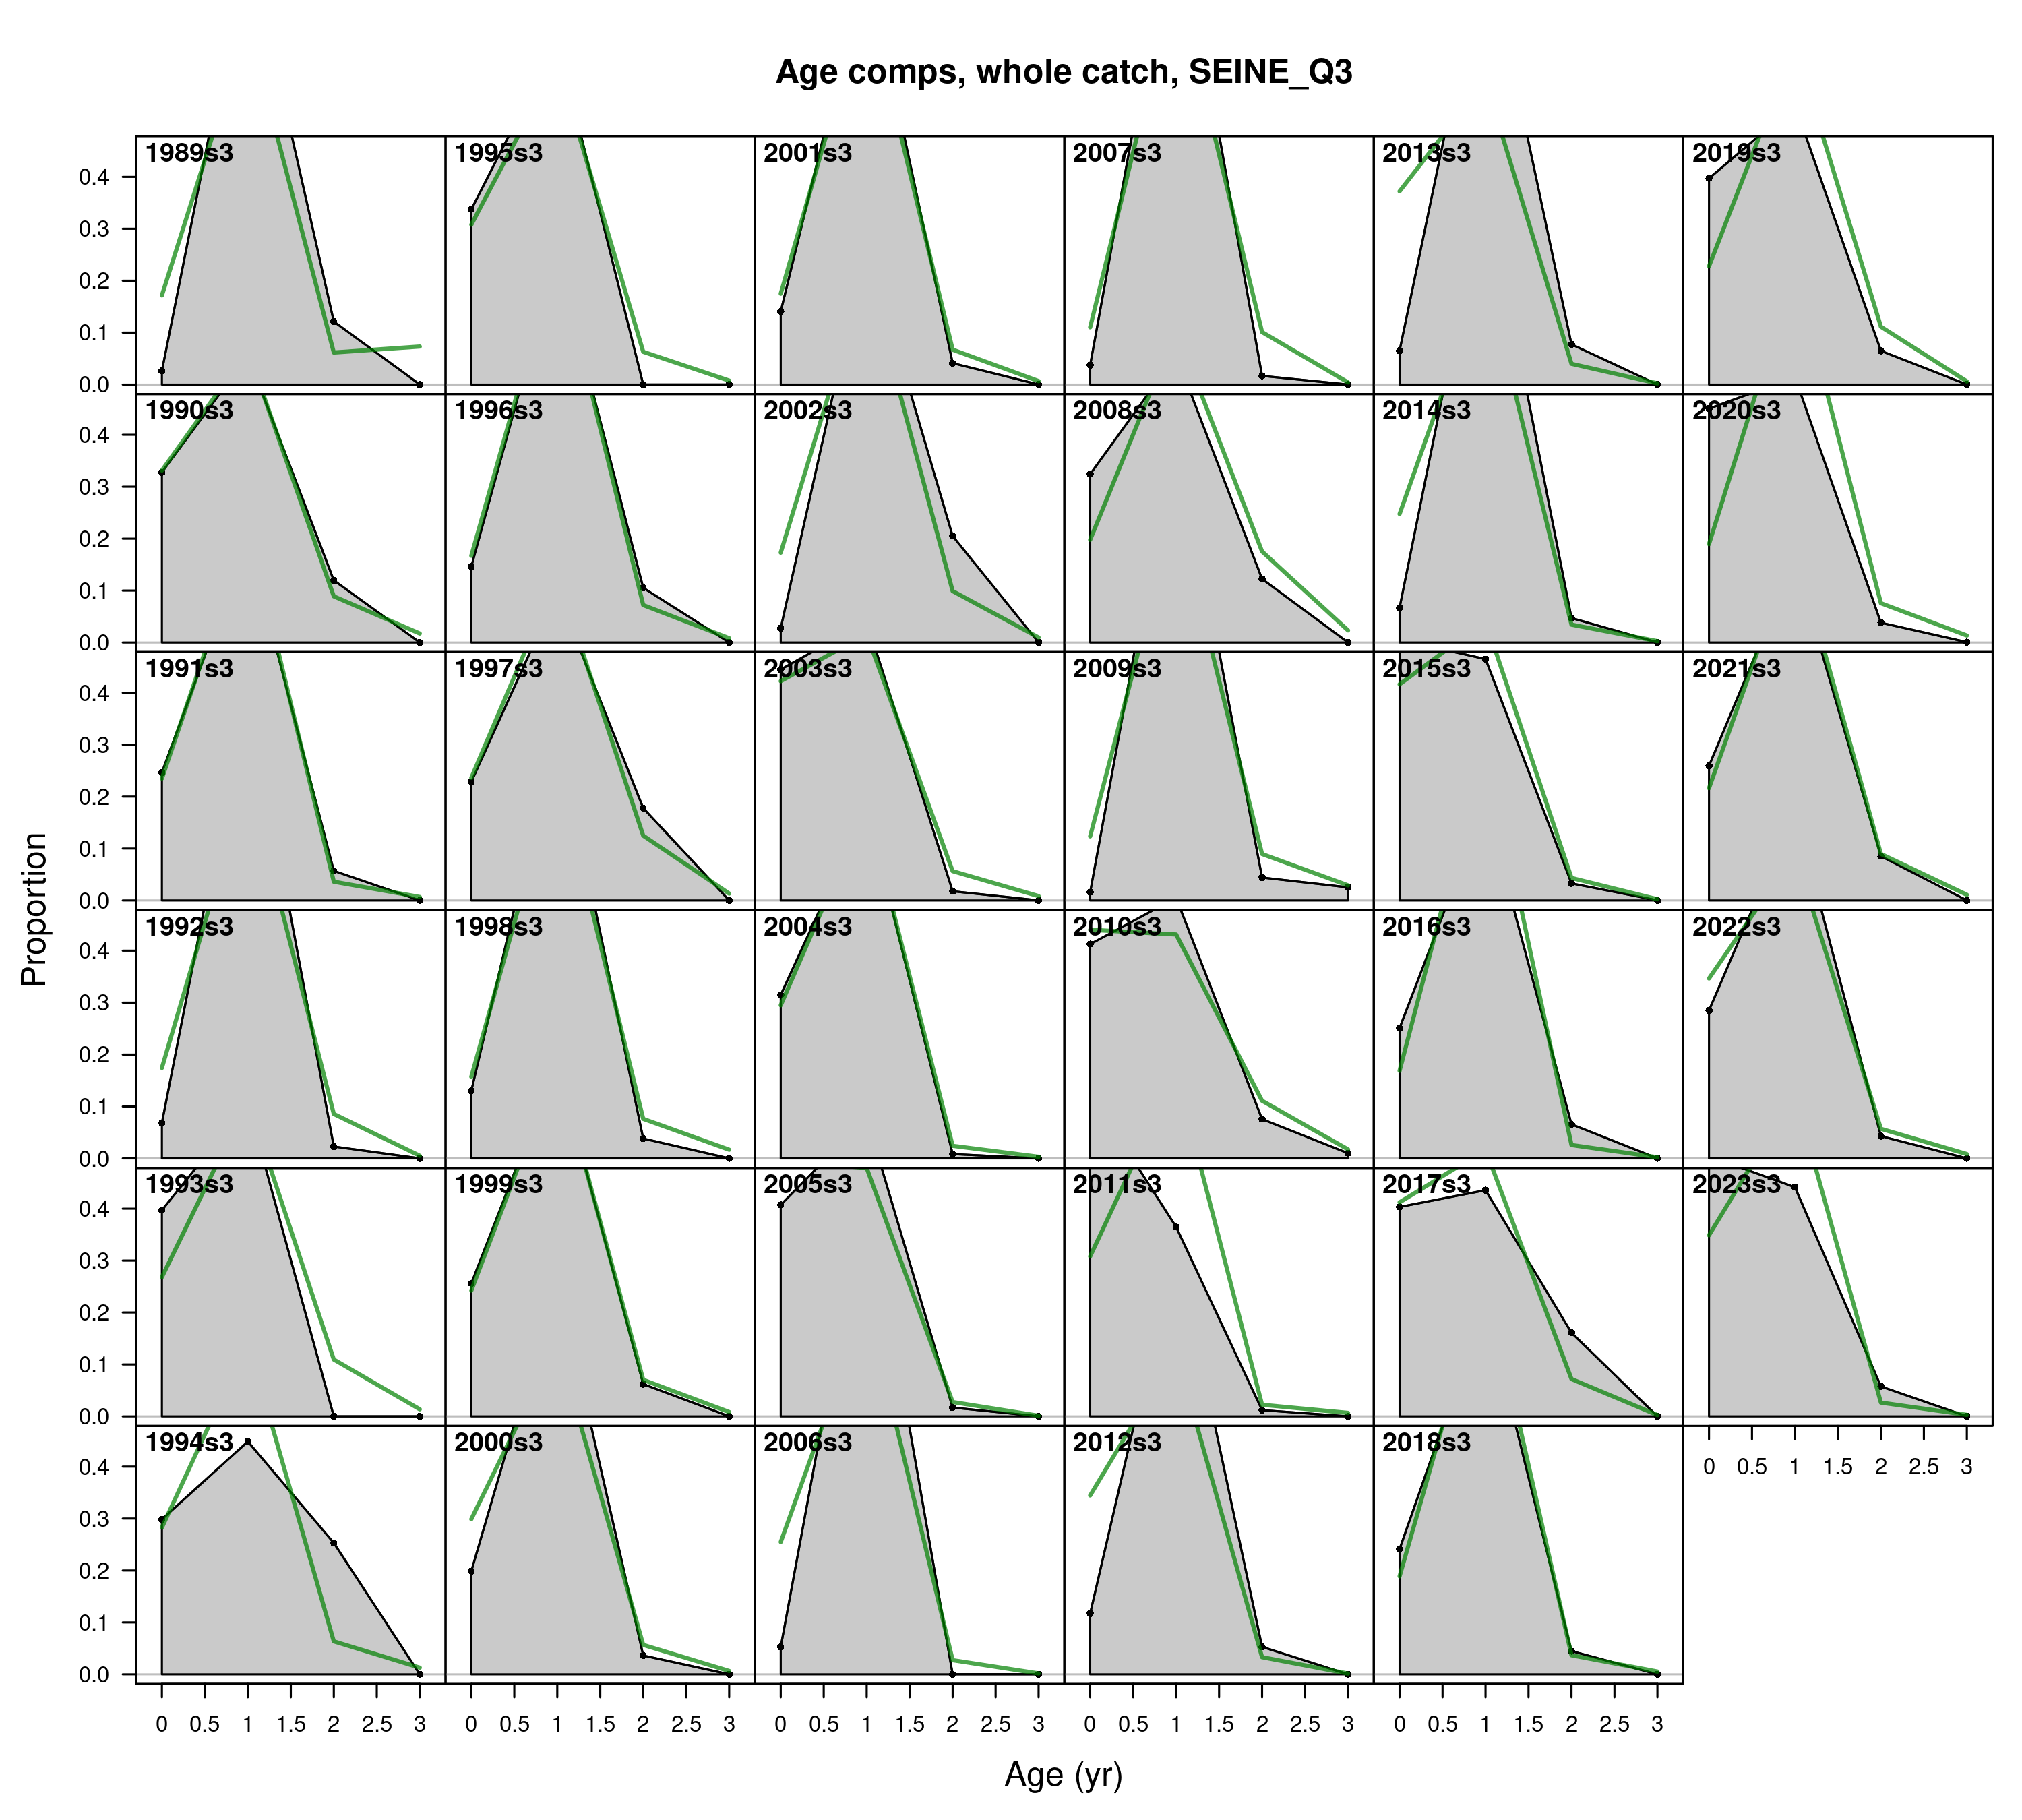
\includegraphics[width=0.95\linewidth]{report/run/S1.0_4FLEETS/fig_age_fit_SeineQ3} 

}

\caption{ane.27.9a stock. Model fit to the age composition data from the *SEINEQ3* fishery, by year and quarter. The green line represents the model estimates, while the shaded grey area shows the observed data.}\label{fig:unnamed-chunk-21}
\end{figure}

\begin{figure}[H]

{\centering 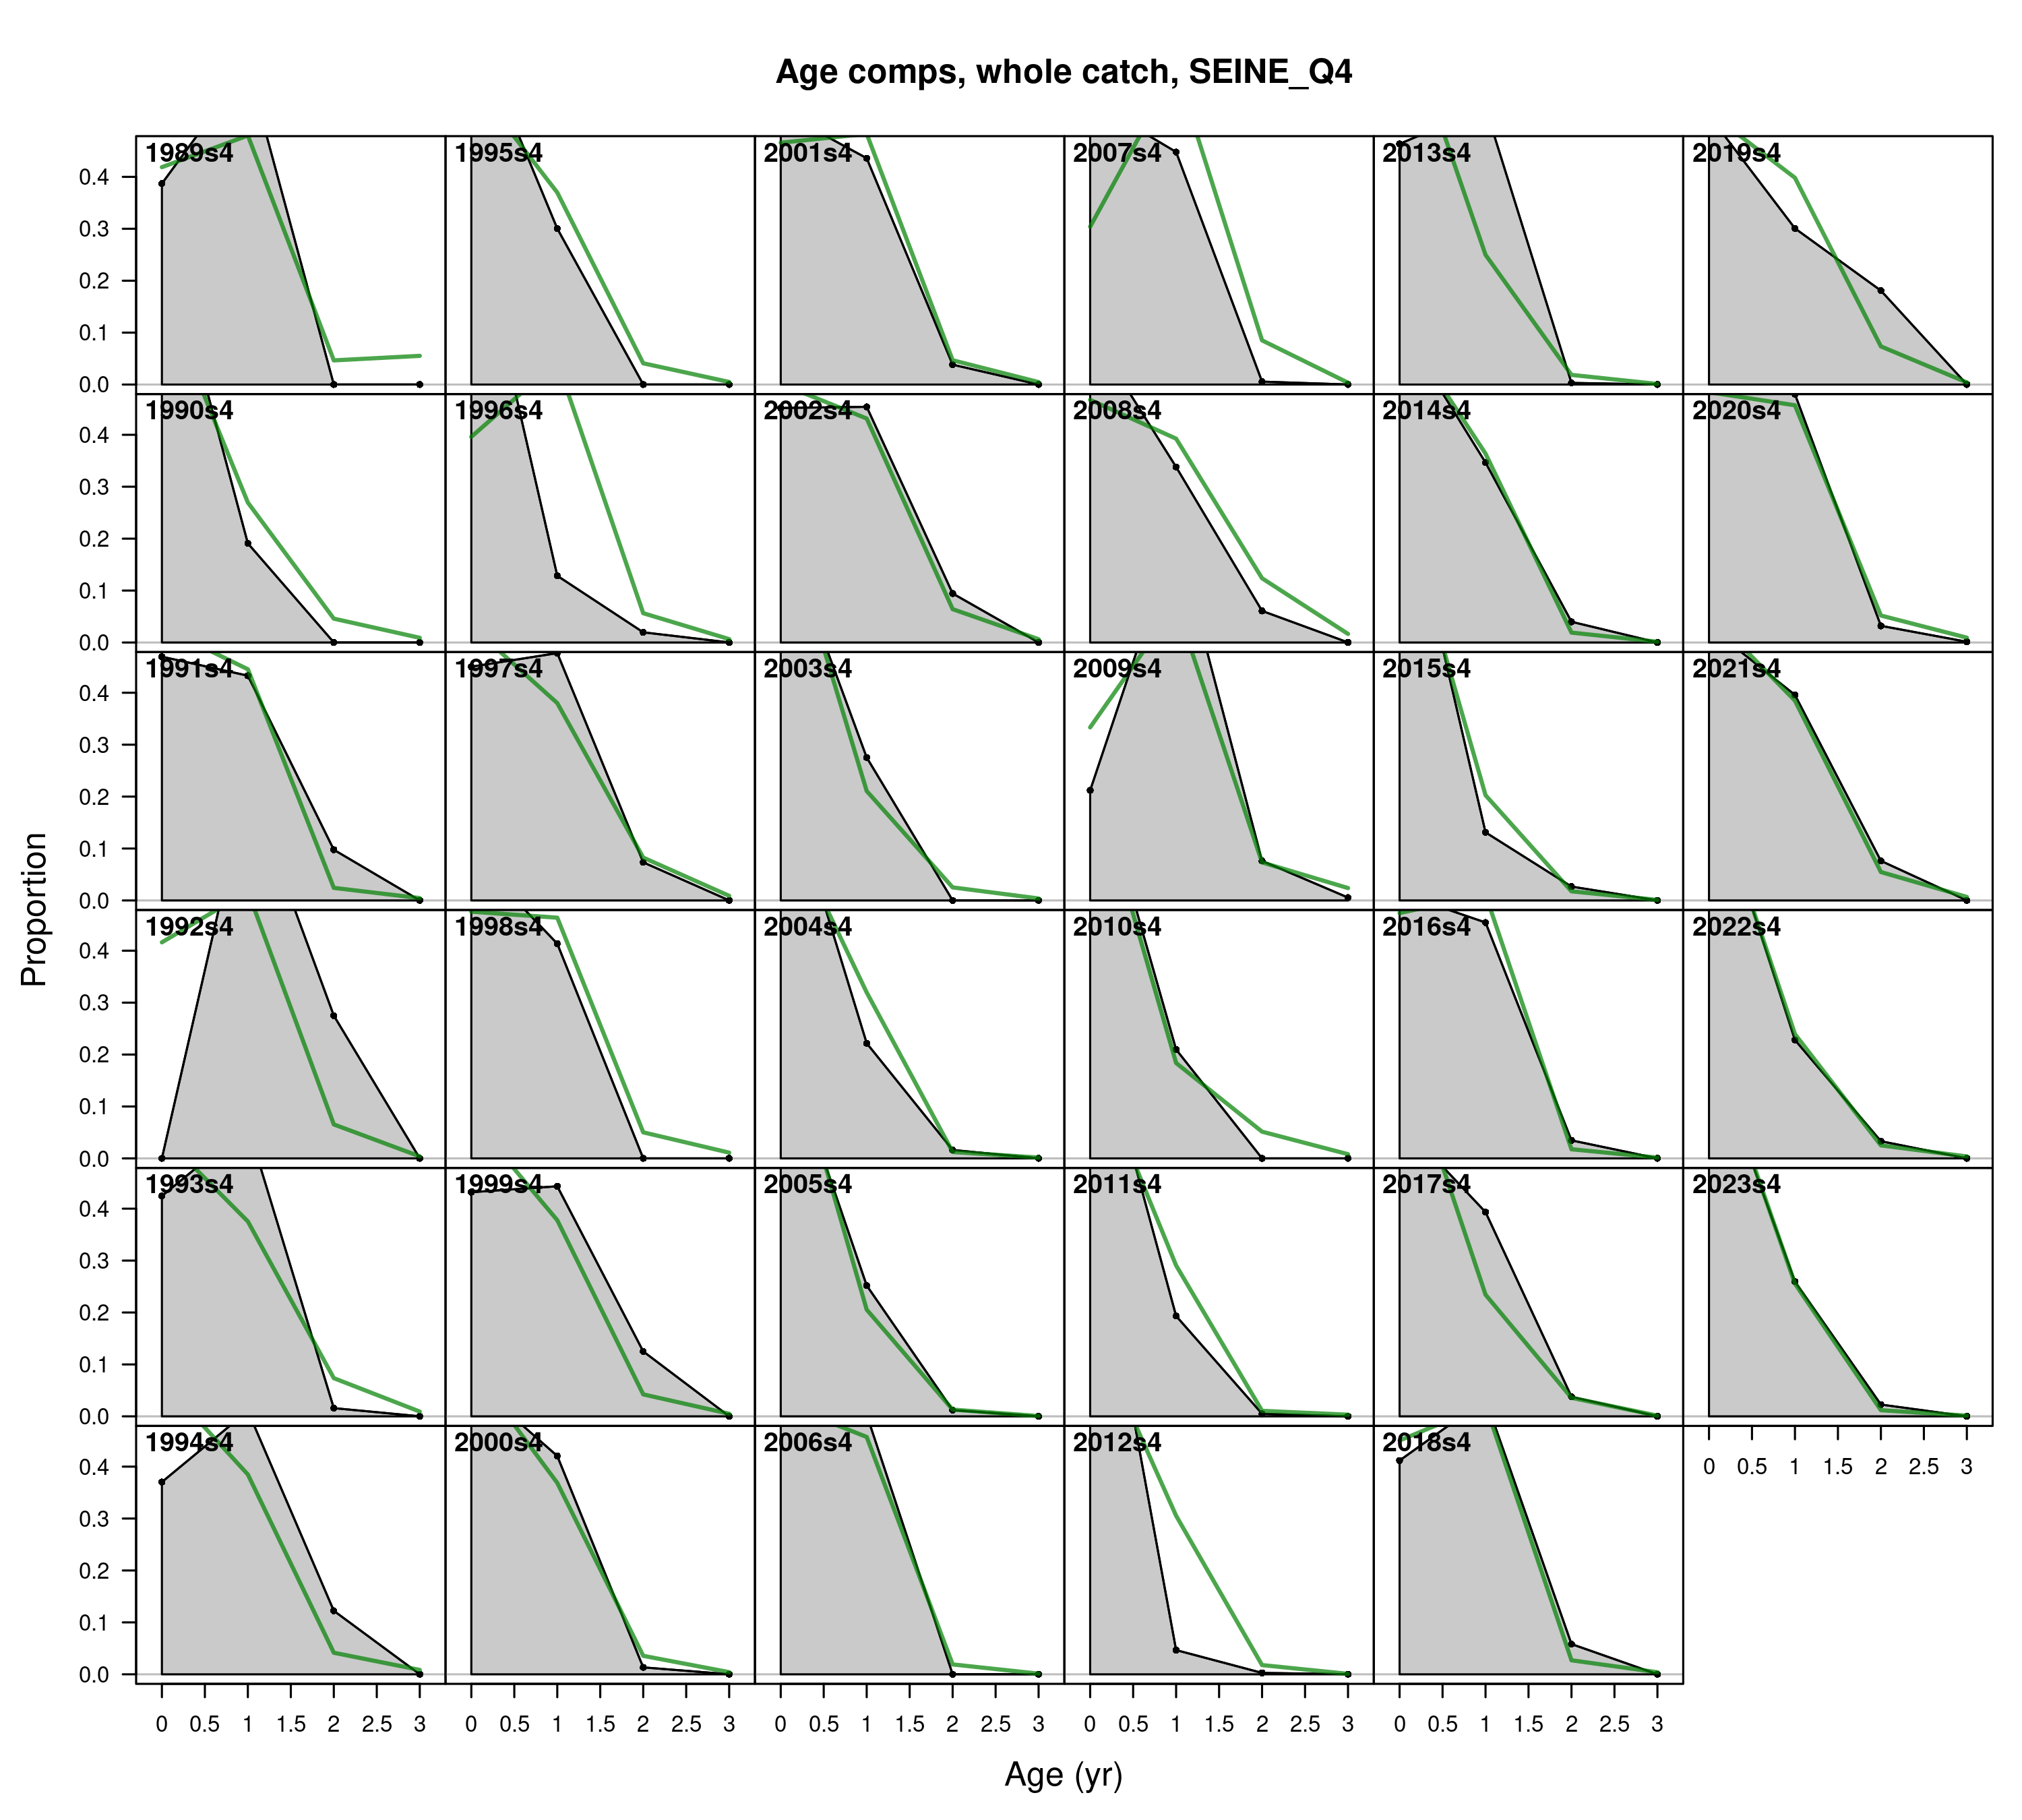
\includegraphics[width=0.95\linewidth]{report/run/S1.0_4FLEETS/fig_age_fit_SeineQ4} 

}

\caption{ane.27.9a stock. Model fit to the age composition data from the *SEINEQ4* fishery, by year and quarter. The green line represents the model estimates, while the shaded grey area shows the observed data.}\label{fig:unnamed-chunk-22}
\end{figure}

\begin{figure}[H]

{\centering 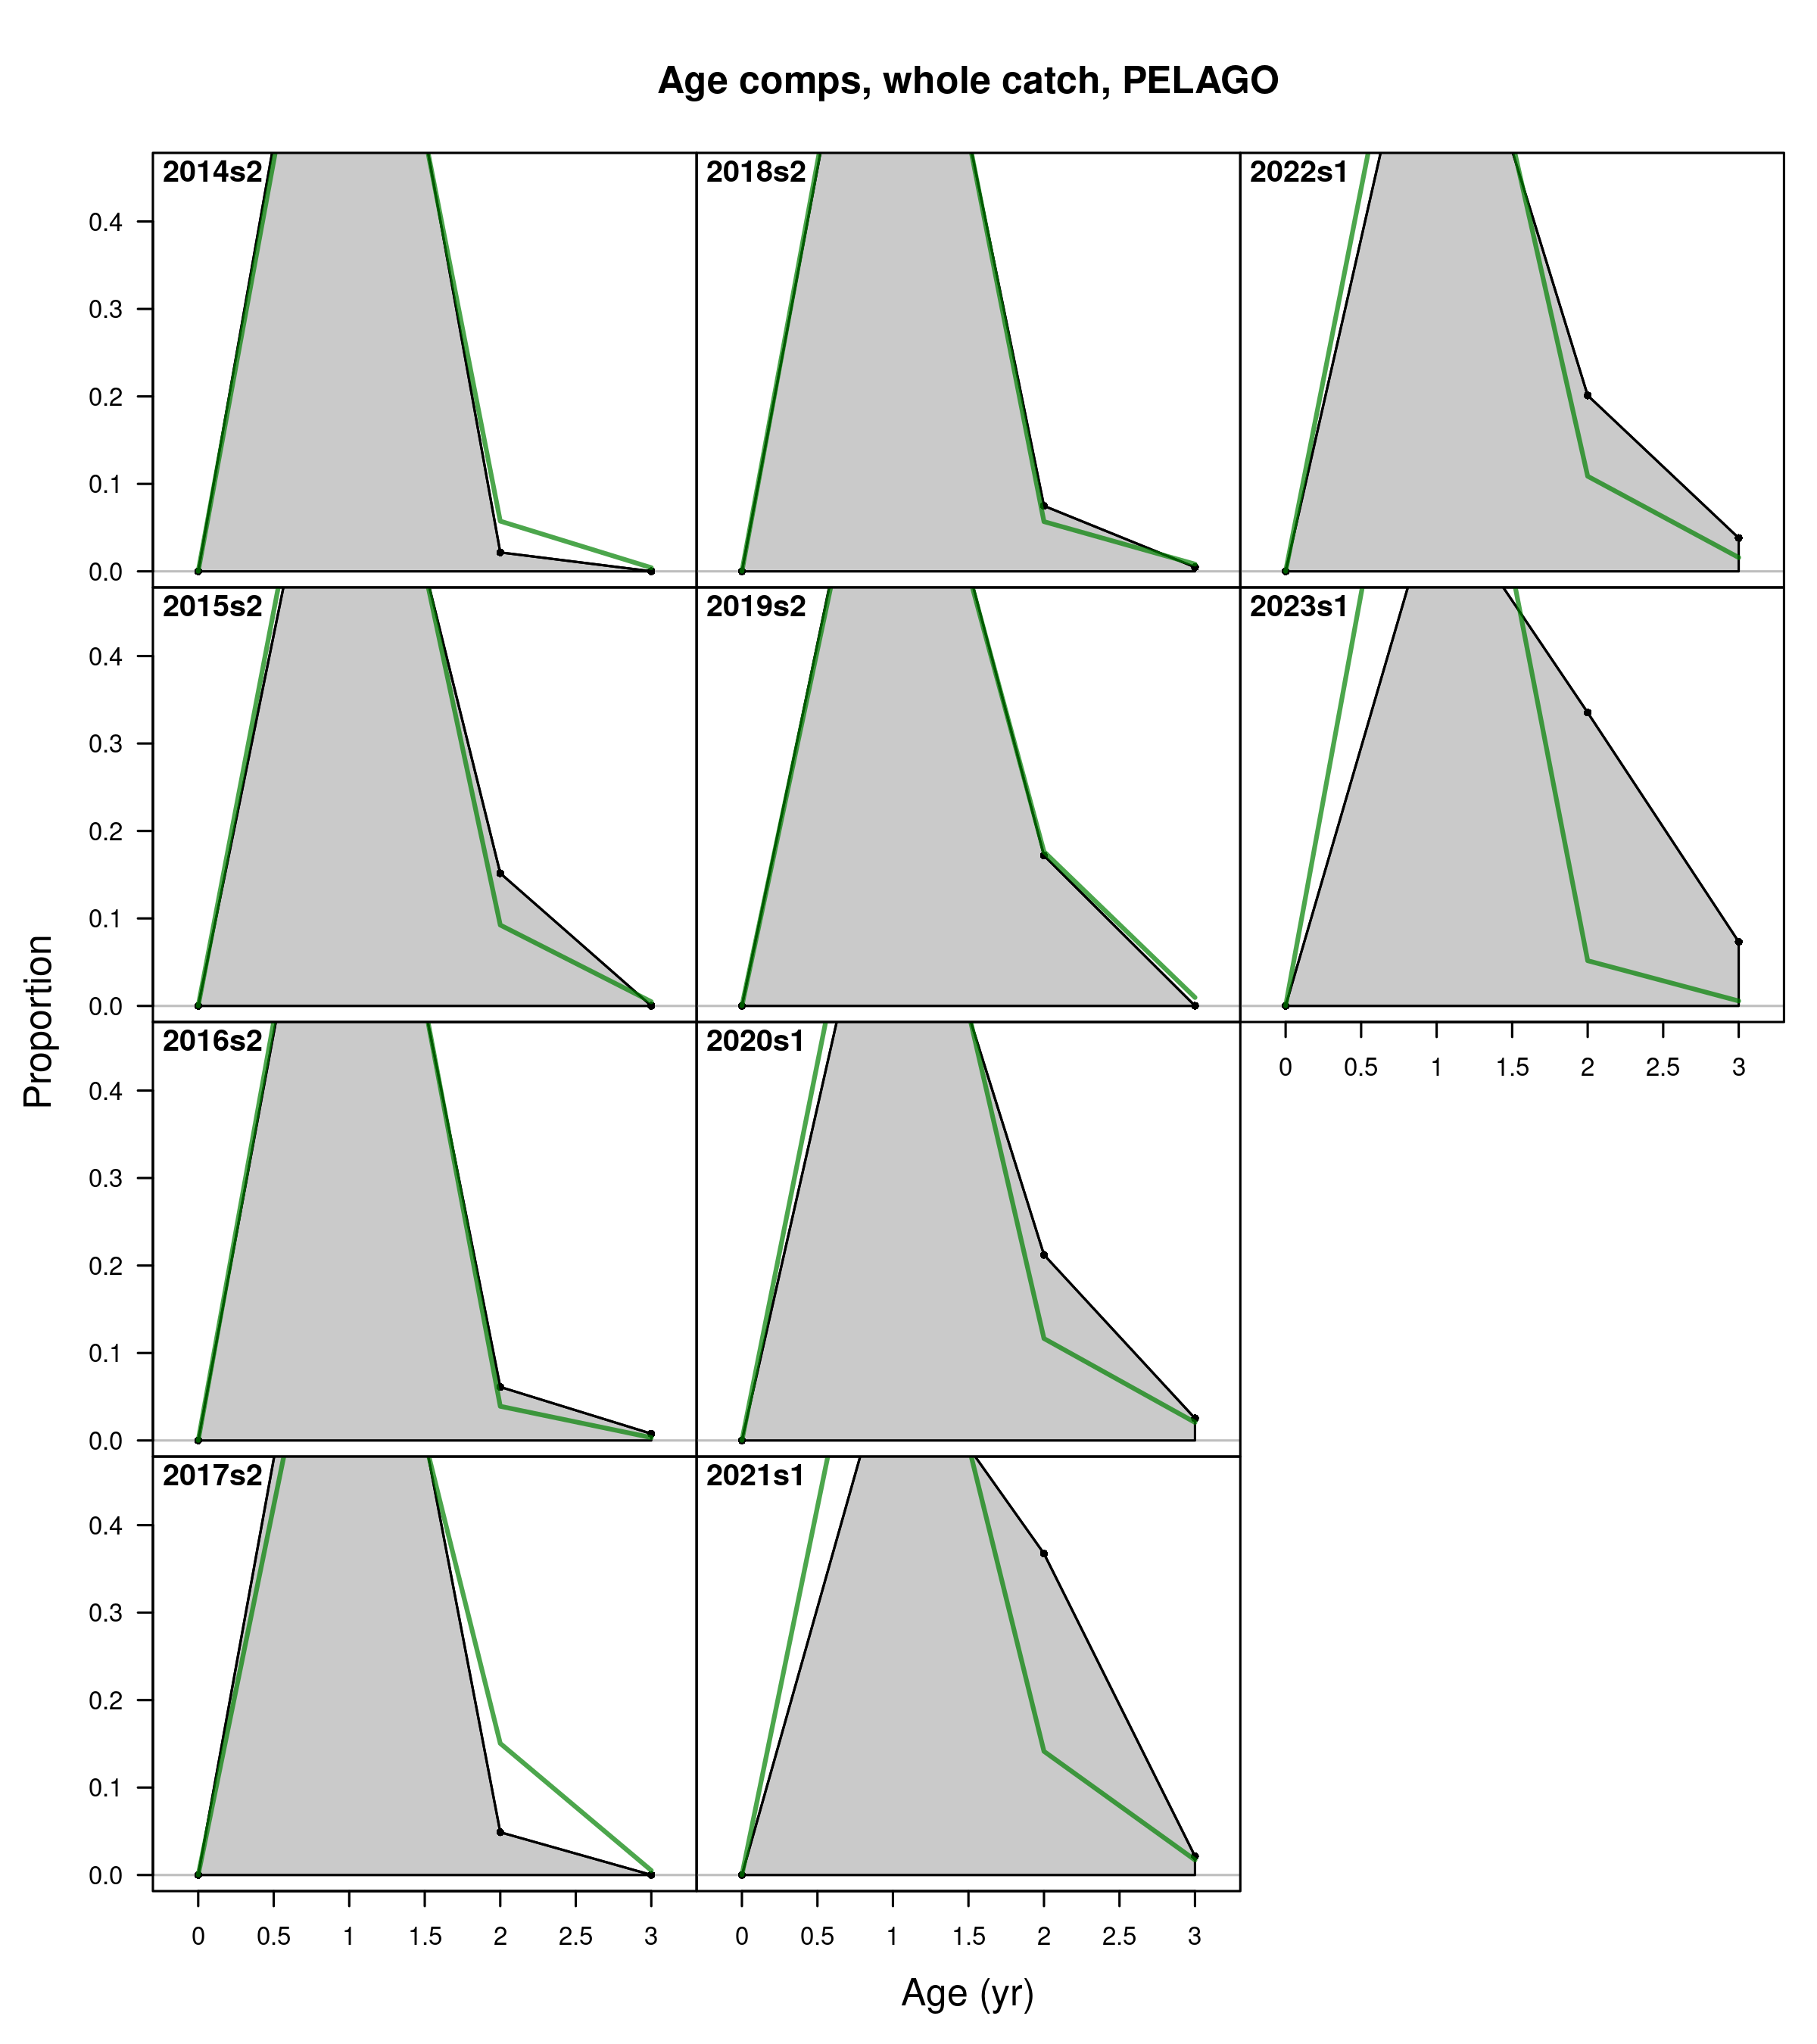
\includegraphics[width=0.95\linewidth]{report/run/S1.0_4FLEETS/fig_age_fit_Pelago} 

}

\caption{ane.27.9a stock. Model fit to the age composition data from the *PELAGO* spring survey by year. The green line represents the model estimates, while the shaded grey area shows the observed data.}\label{fig:unnamed-chunk-23}
\end{figure}

\begin{figure}[H]

{\centering 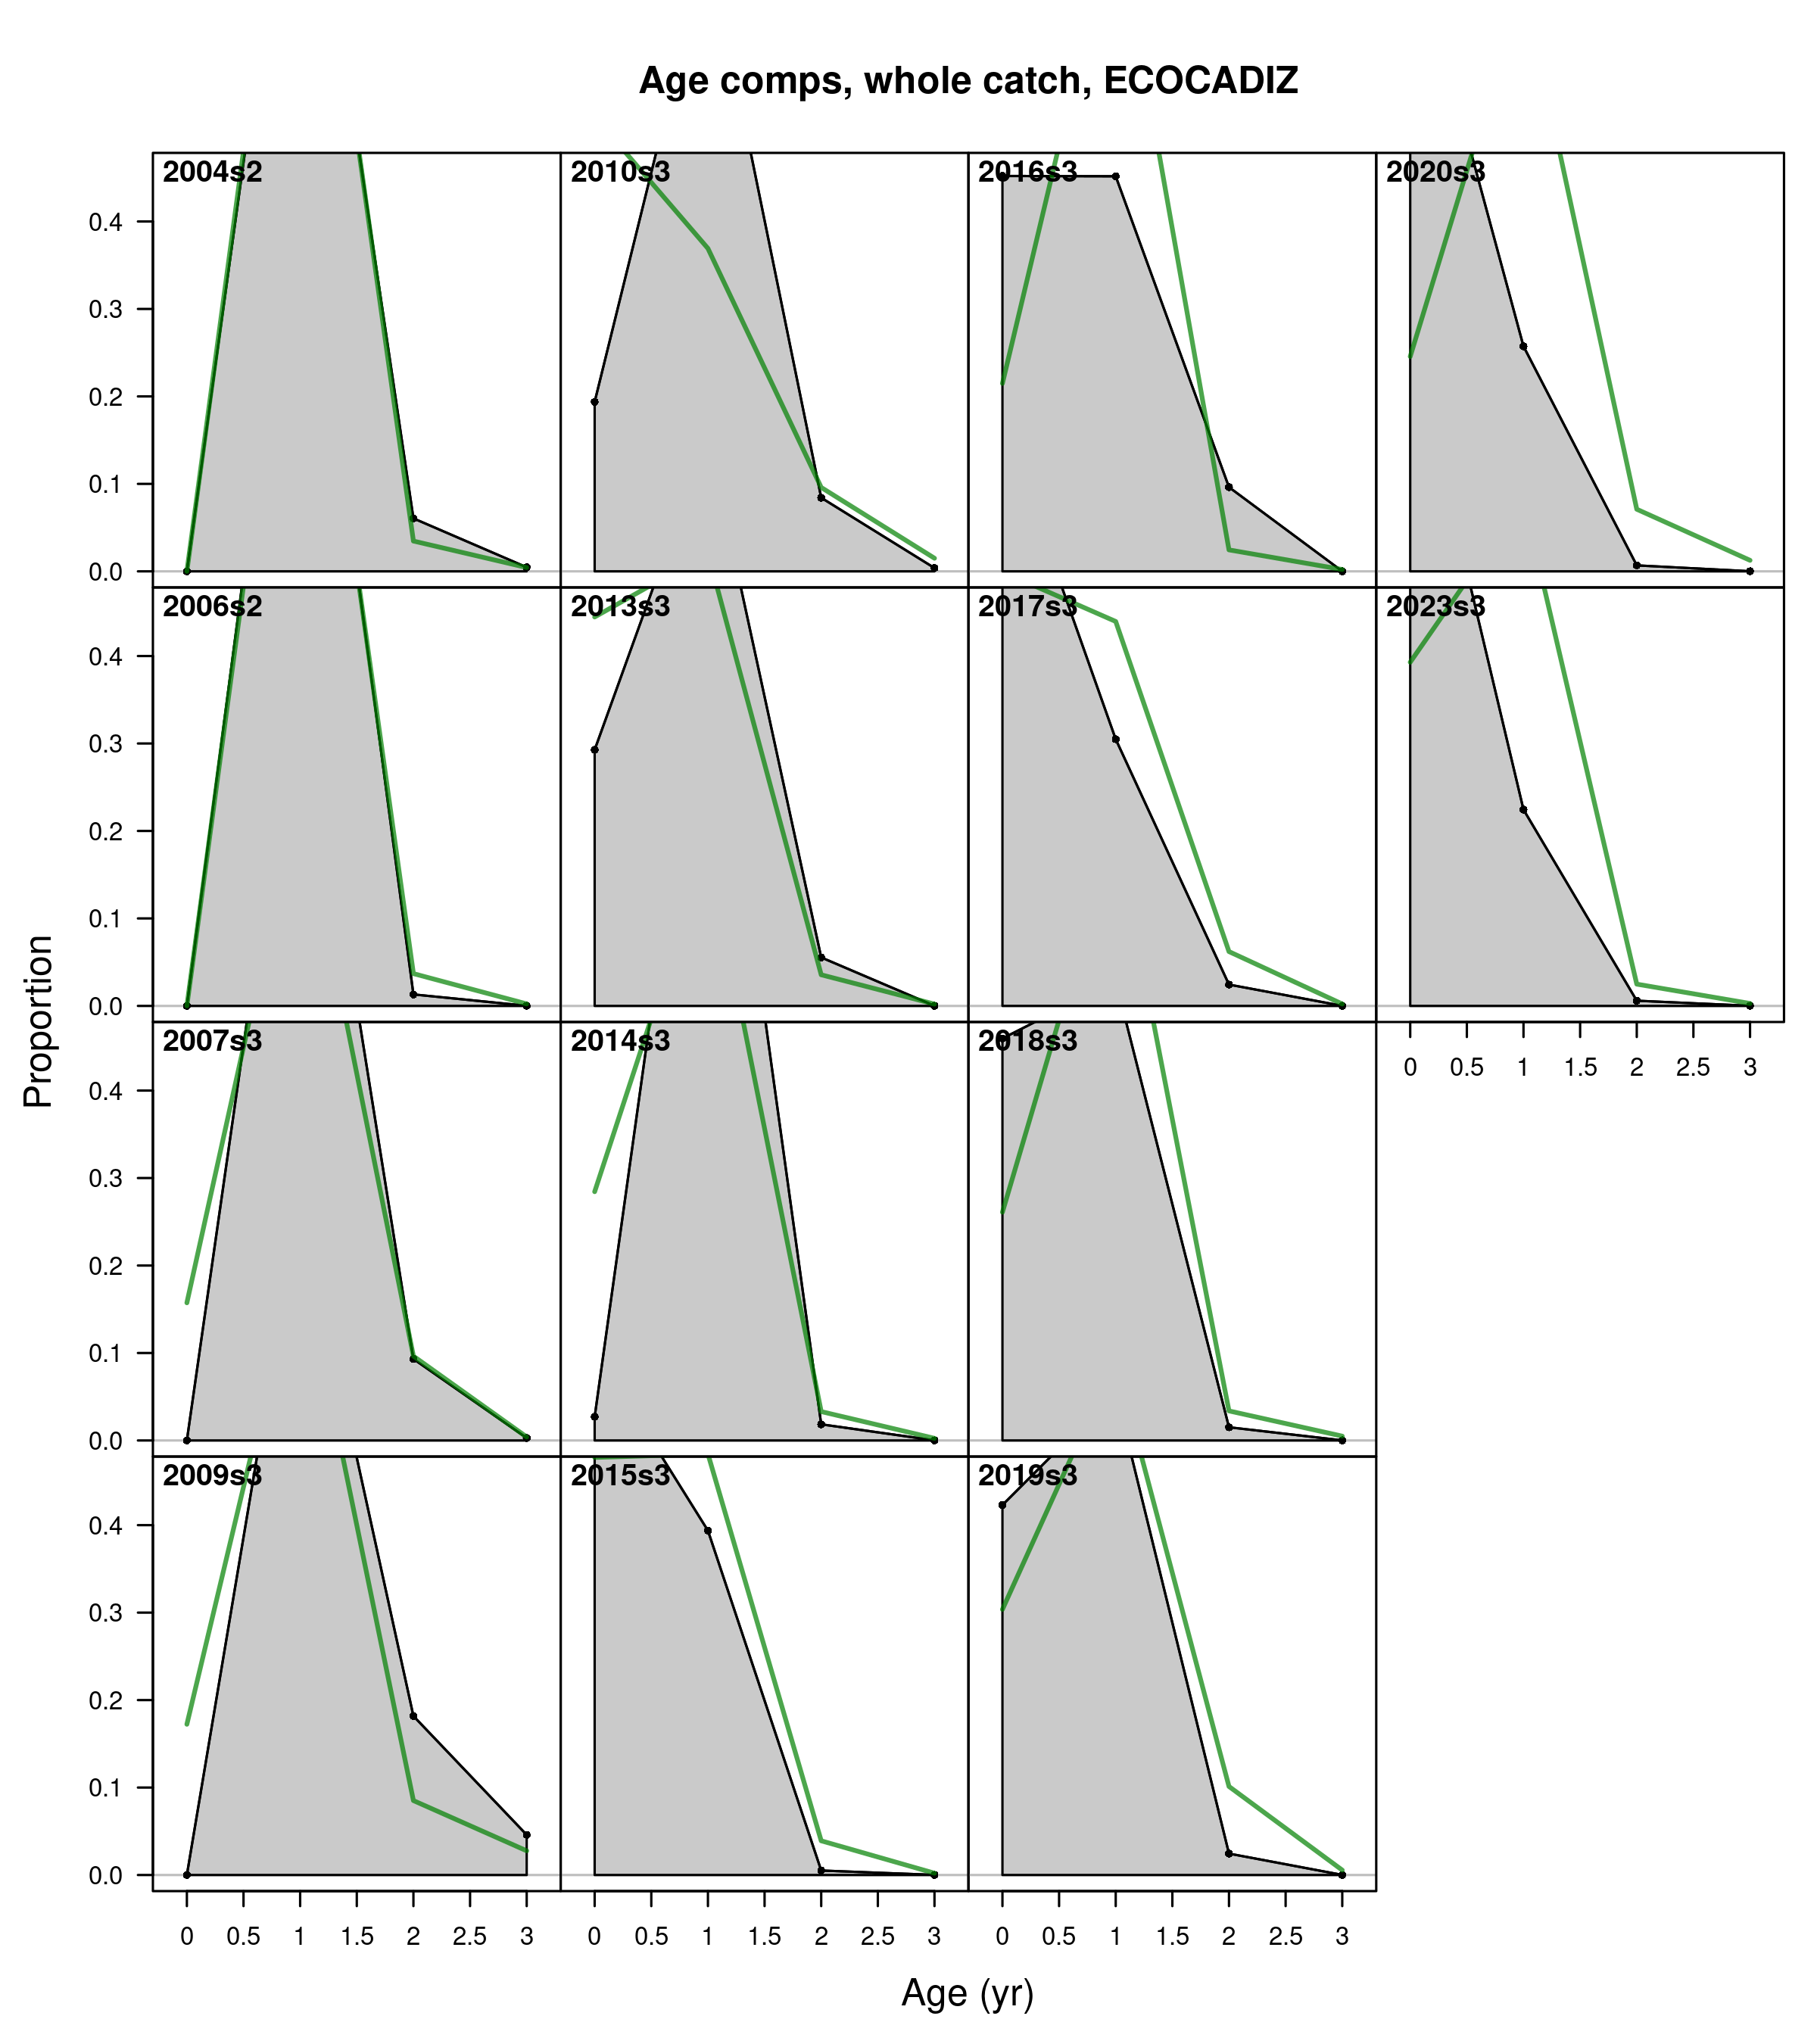
\includegraphics[width=0.95\linewidth]{report/run/S1.0_4FLEETS/fig_age_fit_Ecocadiz} 

}

\caption{ane.27.9a stock. Model fit to the age composition data from the *ECOCADIZ* summer survey by year. The green line represents the model estimates, while the shaded grey area shows the observed data.}\label{fig:unnamed-chunk-24}
\end{figure}

\begin{figure}[H]

{\centering 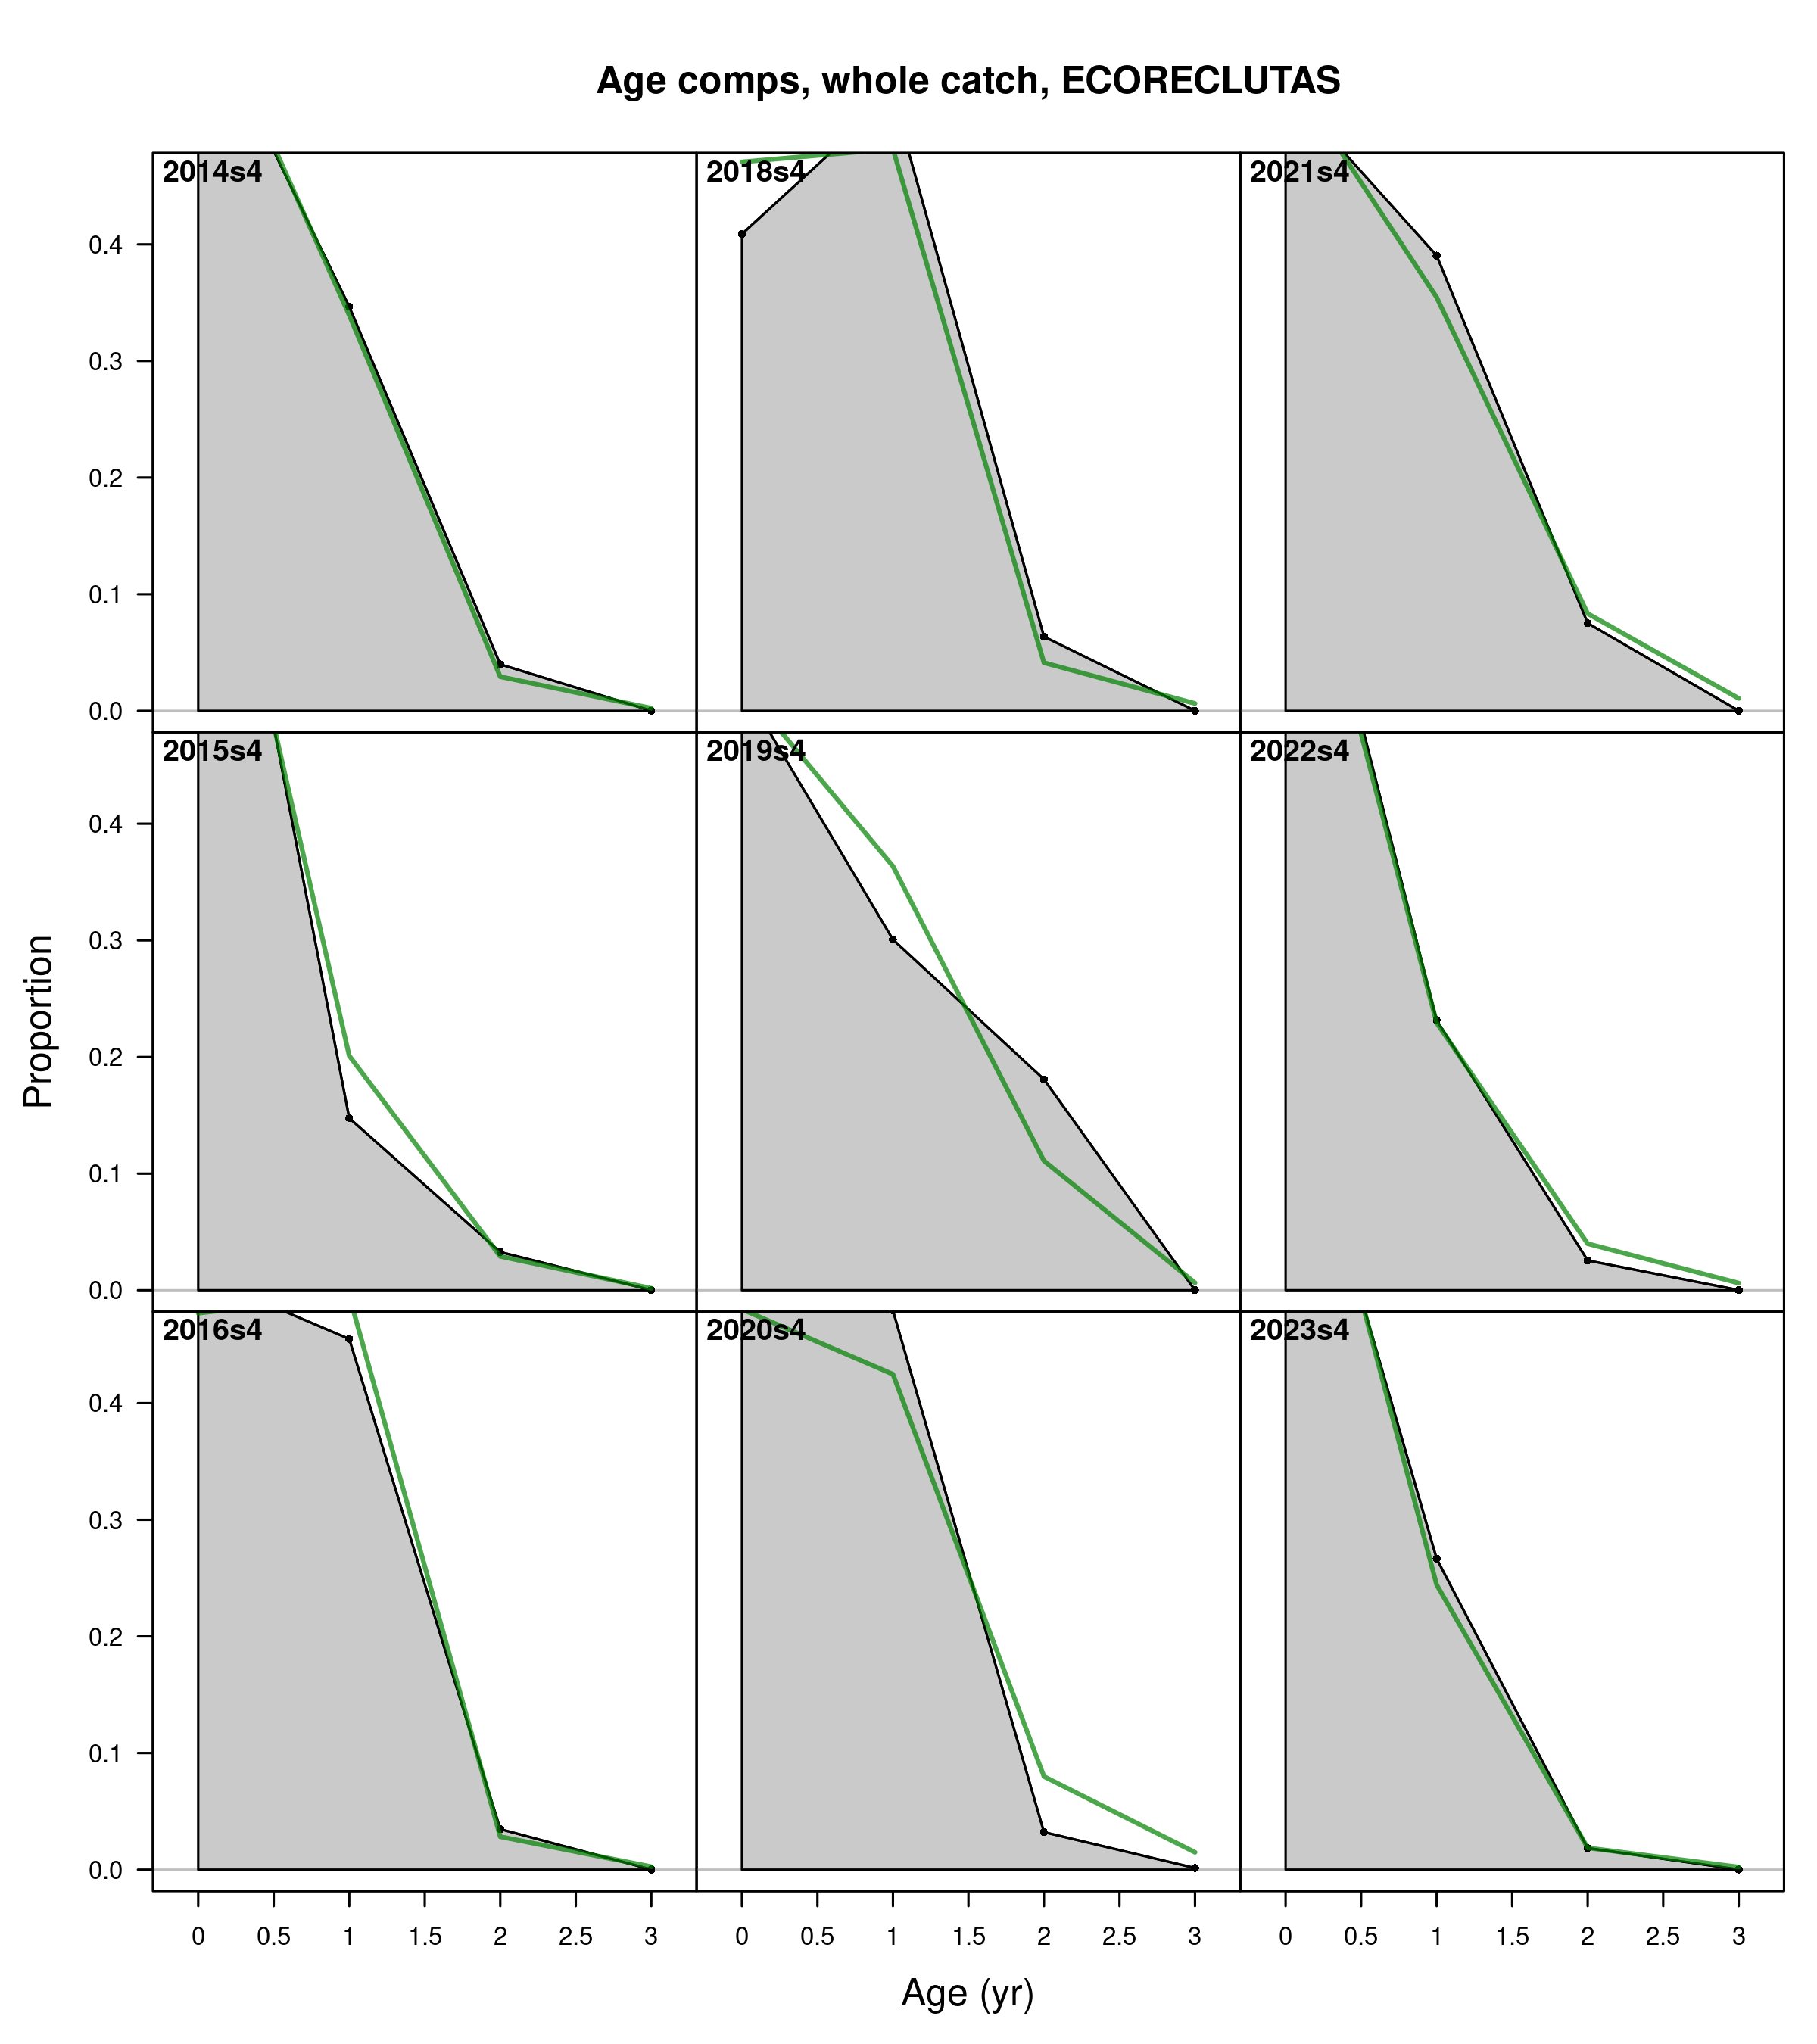
\includegraphics[width=0.95\linewidth]{report/run/S1.0_4FLEETS/fig_age_fit_EcocadizRecl} 

}

\caption{ane.27.9a stock. Model fit to the age composition data from the *ECOCADIZ-RECLUTAS* fall survey by year. The green line represents the model estimates, while the shaded grey area shows the observed data.}\label{fig:unnamed-chunk-25}
\end{figure}

\begin{figure}[H]

{\centering 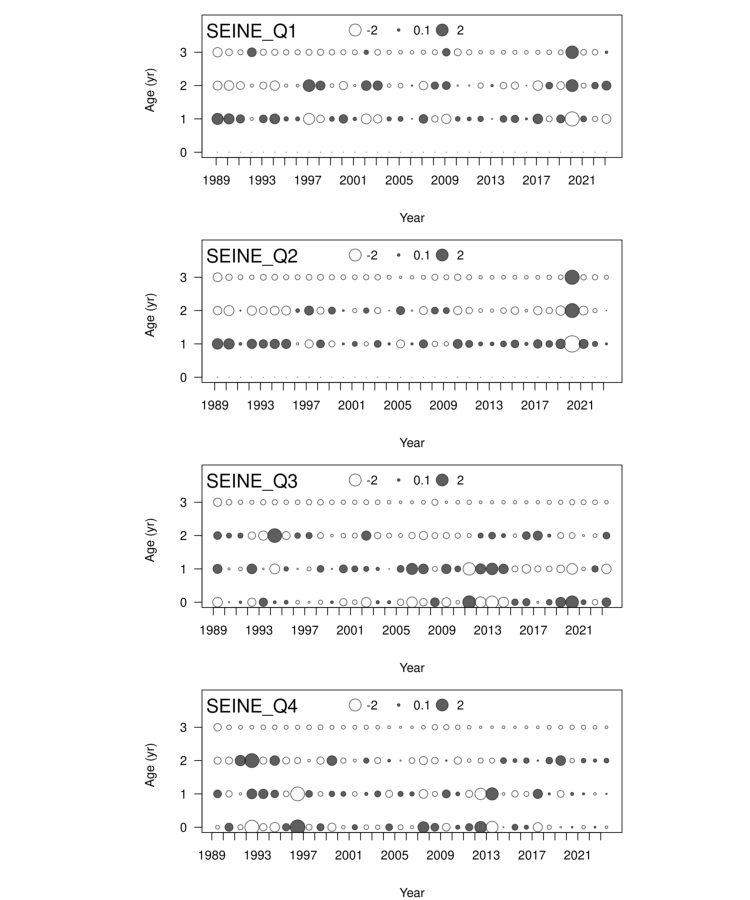
\includegraphics[width=0.95\linewidth]{Report_SS3_quarter_with_age_data_S1.0_4FLEETS_files/figure-latex/unnamed-chunk-26-1} 

}

\caption{ane.27.9a stock.  Pearson residuals, comparing across fleets. Closed bubbles are positive residuals (observed > expected) and open negative residuals (observed < expected).}\label{fig:unnamed-chunk-26}
\end{figure}

\begin{figure}[H]

{\centering 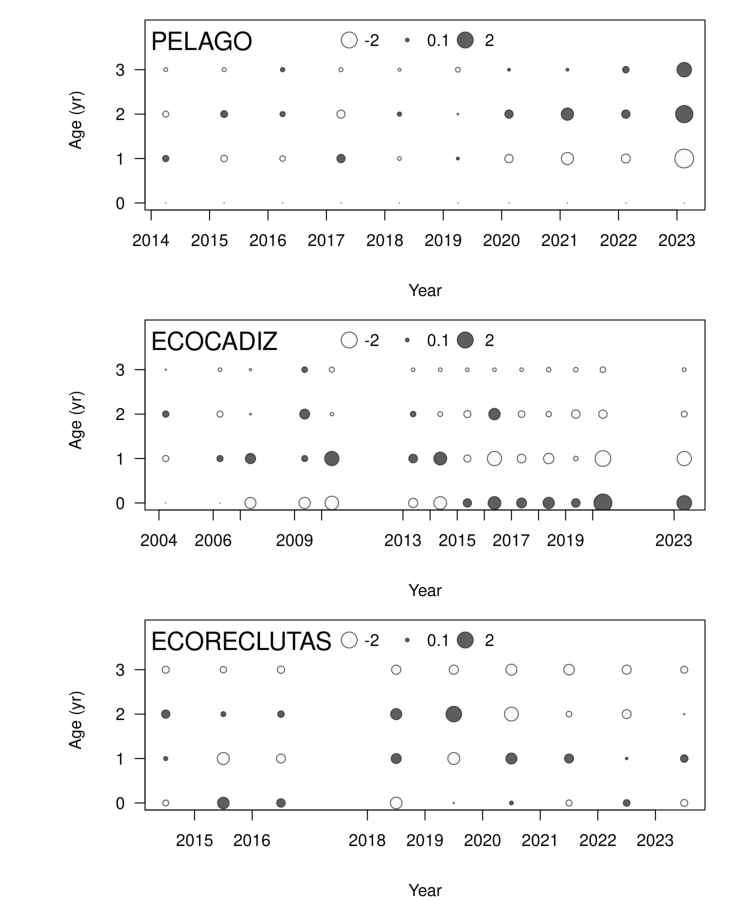
\includegraphics[width=0.95\linewidth]{Report_SS3_quarter_with_age_data_S1.0_4FLEETS_files/figure-latex/unnamed-chunk-27-1} 

}

\caption{ane.27.9a stock.  Pearson residuals, comparing across surveys. Closed bubbles are positive residuals (observed > expected) and open negative residuals (observed < expected).}\label{fig:unnamed-chunk-27}
\end{figure}

The Figure 21 shows that the residuals from the fit of the age
proportions are randomly distributed, with p-values greater than 0.05 in
the case of the commercial fleet (\emph{SEINE}: ) and the acoustic
surveys (\emph{PELAGO}: 0.744, \emph{ECOCADIZ-RECLUTAS}: 0.374). Some
violations of the three-standard-deviation limit are observed for the
commercial fleet (\emph{SEINE}) during the fourth quarter of 1991, 1996,
and 2012, as well as in the \emph{PELAGO} survey in the last year of the
series (2023). In the case of the \emph{ECOCADIZ} survey, the residuals
are not randomly distributed as indicated by a p-value of 0.014, with
several violations of the three-standard-deviation limit observed,
primarily from 2018 to 2023. The estimated root mean square error (RMSE)
for the joint residual analysis is 29.1\%.

\begin{figure}[H]

{\centering 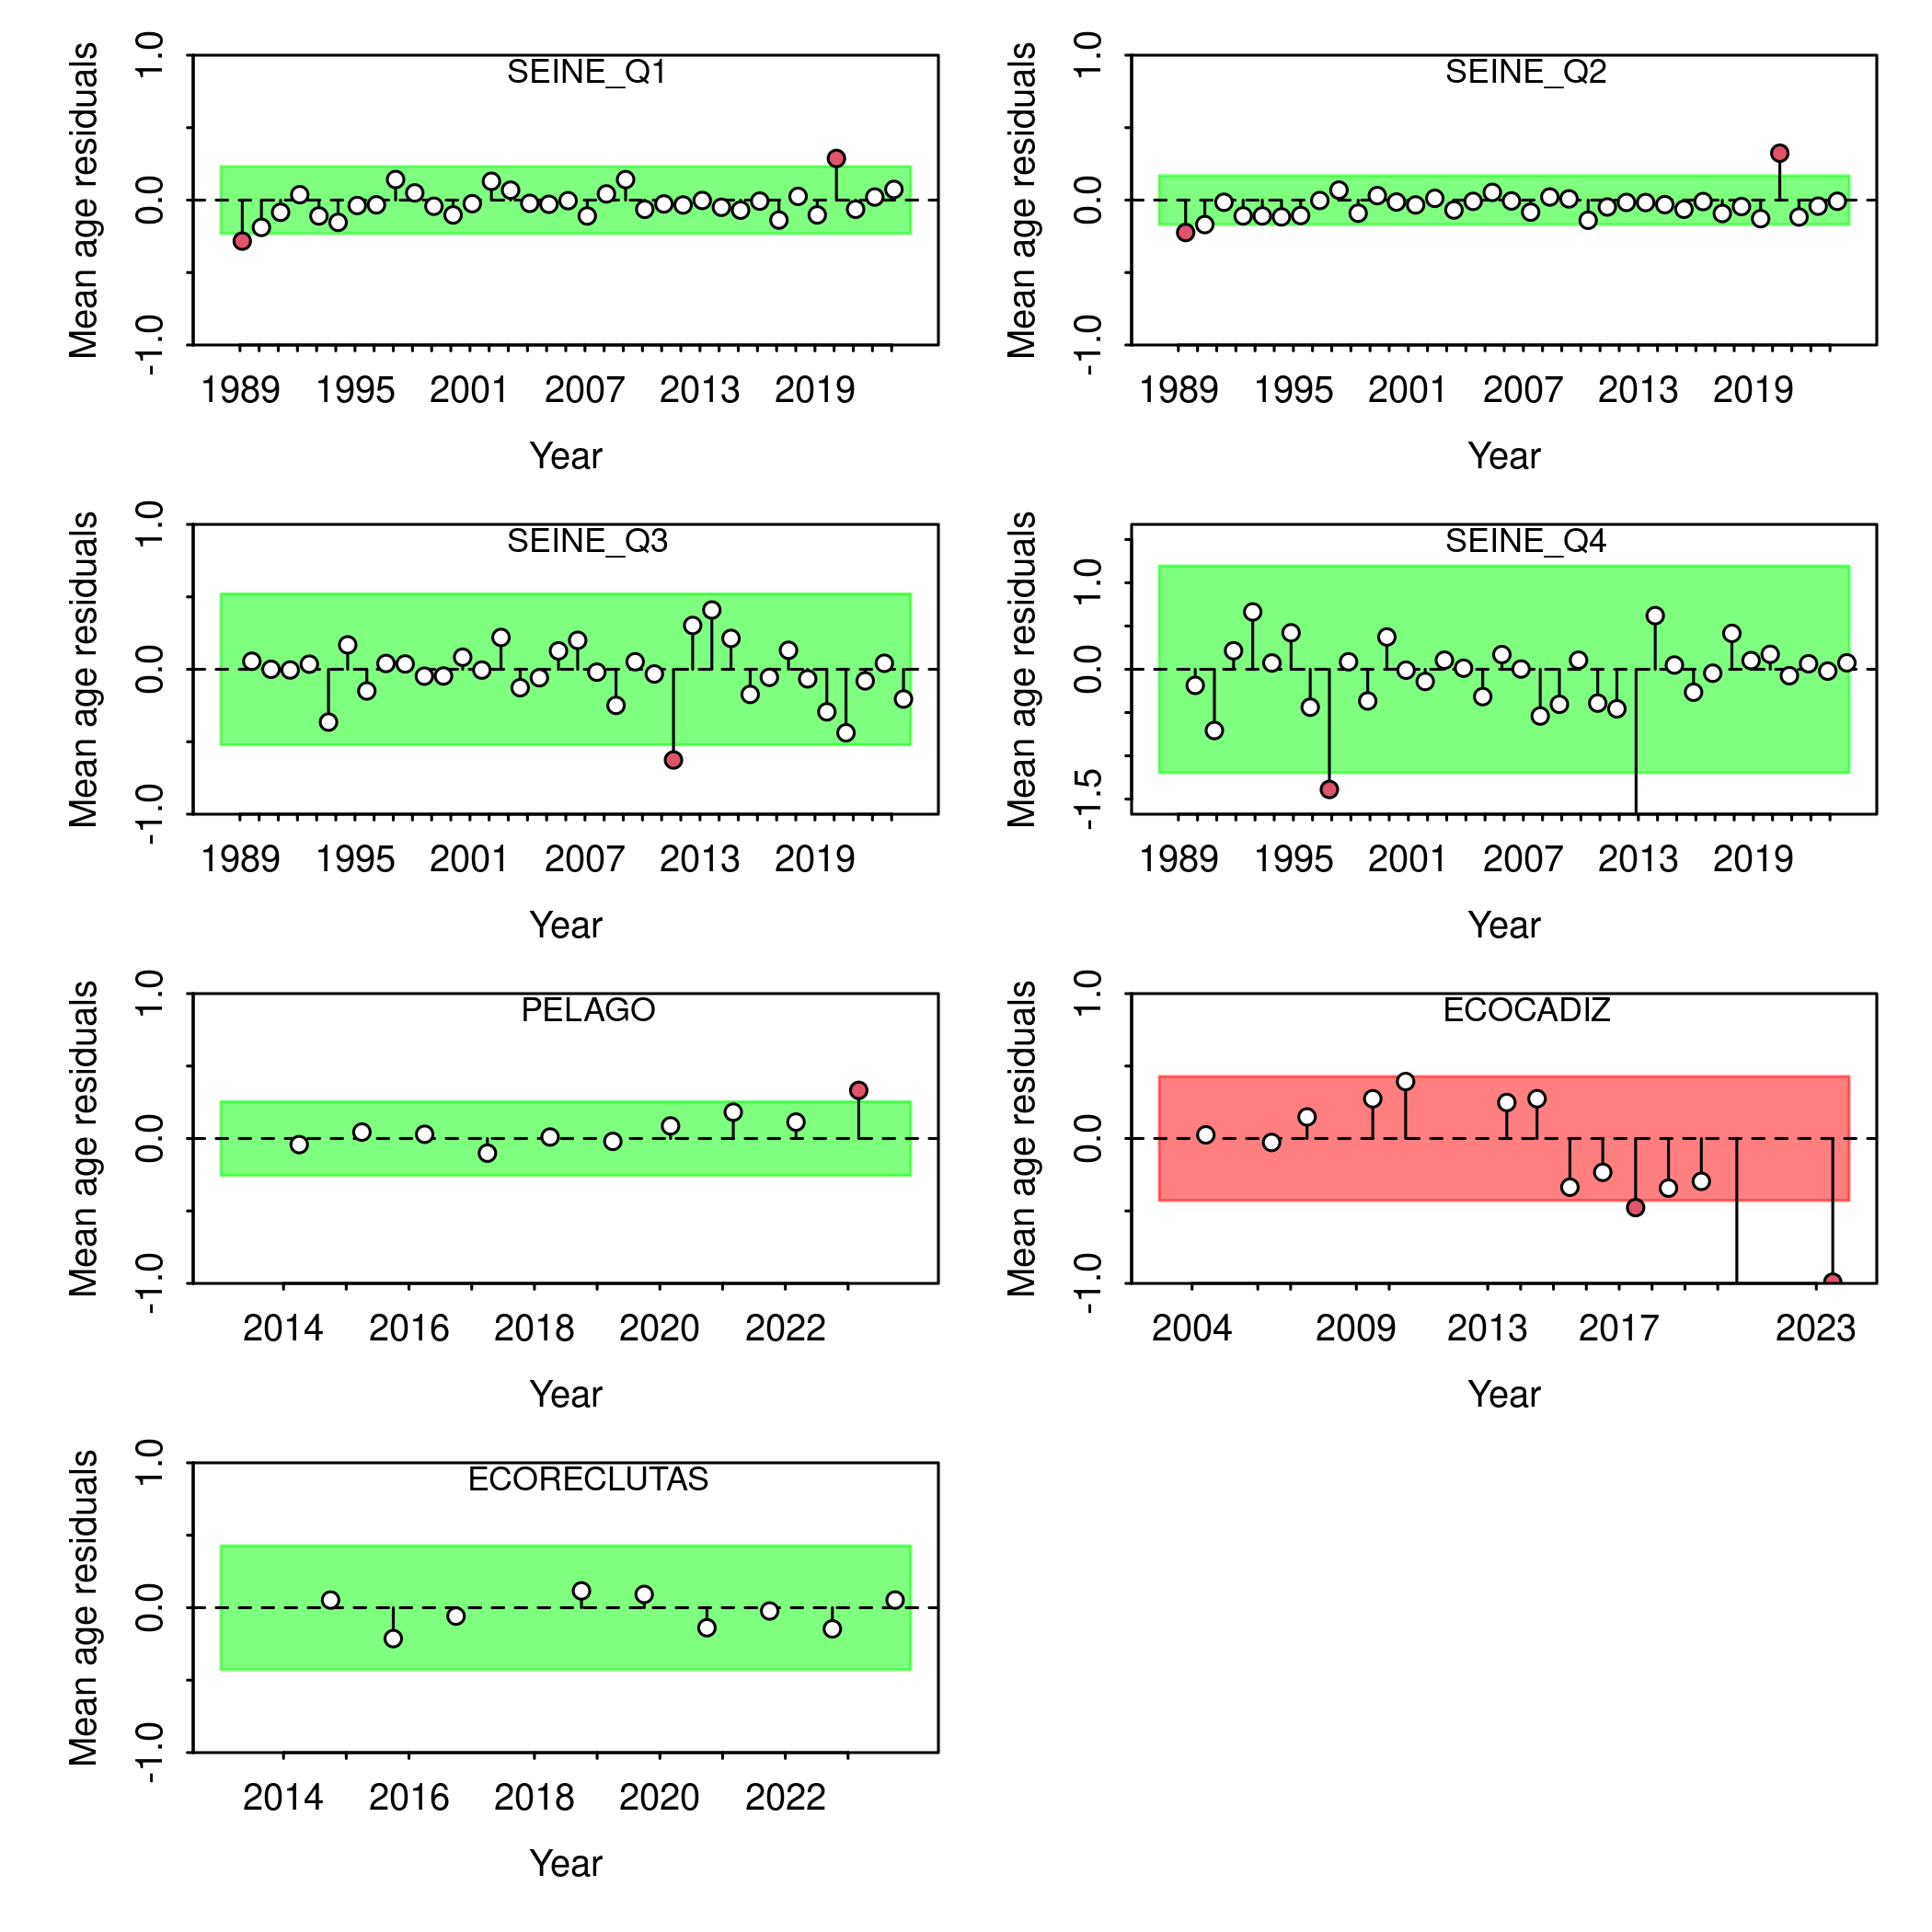
\includegraphics[width=0.95\linewidth]{report/run/S1.0_4FLEETS/fig_runtest_residuals_age} 

}

\caption{ane.27.9a stock. a) Runs test results for fits to annual mean age estimates for the surveys (*PELAGO*, *ECOCADIZ*, *ECOCADIZ-RECLUTAS*) and the fishery (*SEINE*). Green shaded (green/red) area spans three residual standard deviations to either side from zero, and the red points outside of the shading violate the 'three-sigma limit' for that series.  b) Joint residual plots for annual mean length estimates for surveys and fishery (bottom left panel).  Vertical lines with points show the residuals, and the solid black line show loess smoother through all residuals. Root-mean squared error (RMSE) is included in the upper right-hand corner of the panel.}\label{fig:unnamed-chunk-28}
\end{figure}

\hypertarget{retrospective-analysis}{%
\subsection{Retrospective analysis}\label{retrospective-analysis}}

Figure 22 shows a retrospective pattern in both spawning biomass and
fishing mortality in the base model. The retrospective analysis of the
assessment model reveals that, in terms of Mohn's rho (mean of
retrospective anomalies), the reduction in data leads to a pattern of
underestimation in fishing mortality (rho = -0.07933) and overestimation
in spawning biomass (rho = 0.0548217). These Mohn´s rho values were
inside the bounds of recommended values, according to the rule proposed
by Hurtado-Ferro \emph{et al.} (2014), which states that Mohn's rho
index values should be less than 0.30 and greater than -0.22 for
short-lived species.

\begin{figure}[H]

{\centering 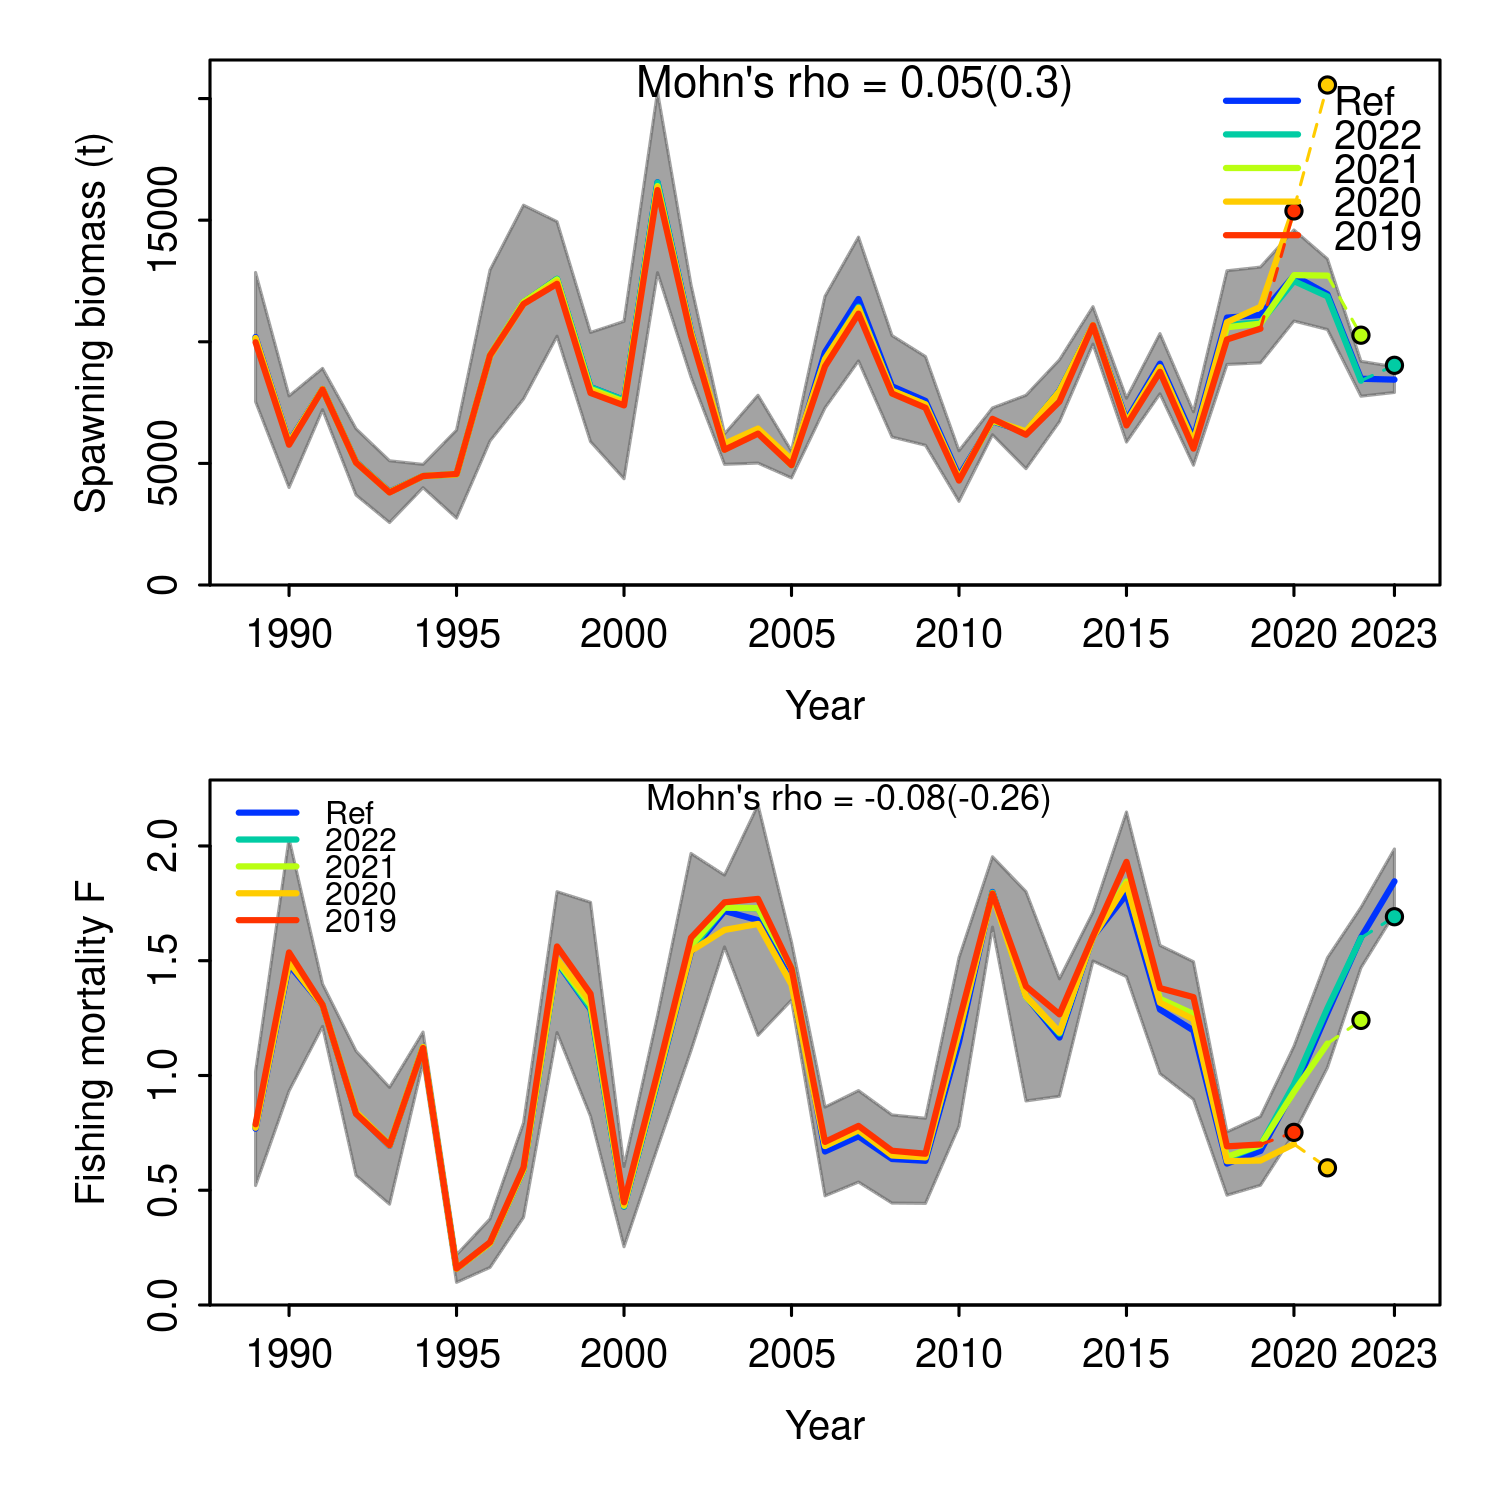
\includegraphics[width=0.95\linewidth]{report/retro/S1.0_4FLEETS/Retro} 

}

\caption{ane.27.9a stock. Retrospective analysis of spawning stock biomass (SSB) and fishing mortality (F). Models  conducted by re-fitting the reference model (Ref) after removing five years of observations, one year at a time sequentially. The retrospective results are shown the entire time series. Mohn's rho statistic and the corresponding 'hindcast rho' values (in brackets) are printed at the top of the panels. One-year-ahead projections denoted by color-coded dashed lines with terminal points are shown for each model. Grey shaded areas are the 95\% confidence intervals from the reference model.}\label{fig:unnamed-chunk-29}
\end{figure}

\hypertarget{results}{%
\section{Results}\label{results}}

\hypertarget{recruitment-deviations}{%
\section{Recruitment deviations}\label{recruitment-deviations}}

\begin{figure}[H]

{\centering 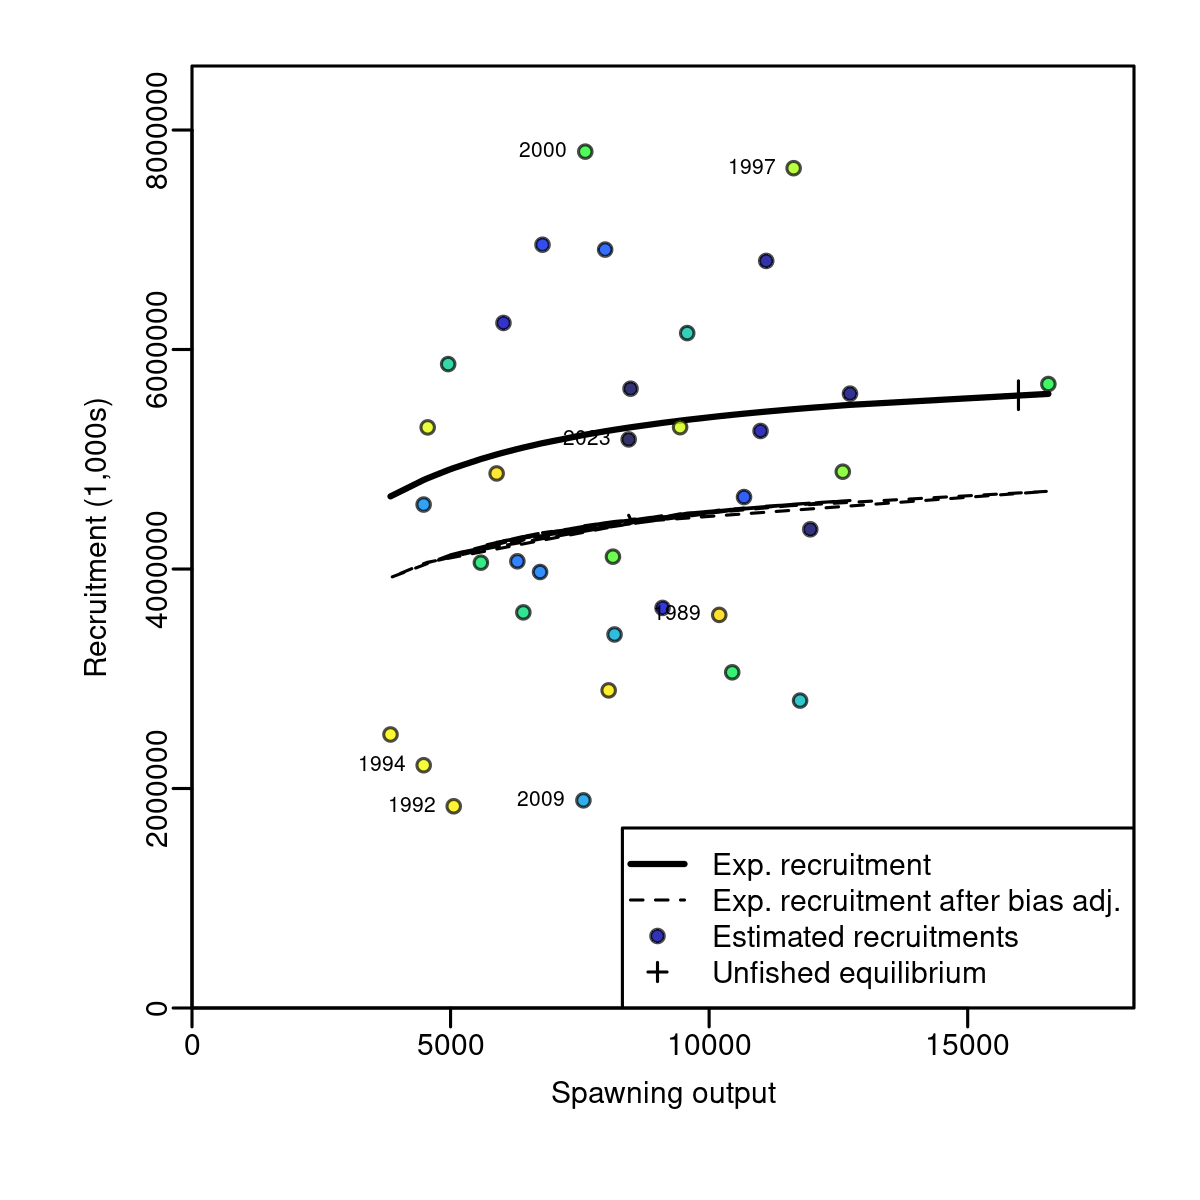
\includegraphics[width=0.95\linewidth]{report/run/S1.0_4FLEETS/fig_stock-recluta} 

}

\caption{ane.27.9a stock. Stock-recruit curve with labels on first, last, and years with (log) deviations > 0.5. Point colors indicate year, with warmer colors indicating earlier years and cooler colors in showing later years..}\label{fig:unnamed-chunk-30}
\end{figure}

\hypertarget{stock-recruitment-relationship}{%
\section{Stock-recruitment
relationship}\label{stock-recruitment-relationship}}

Equilibrium recruitment (\(R_0\)) were estimated in the base model, and
steepness (h) was fixed at 0.8.

\begin{figure}[H]

{\centering 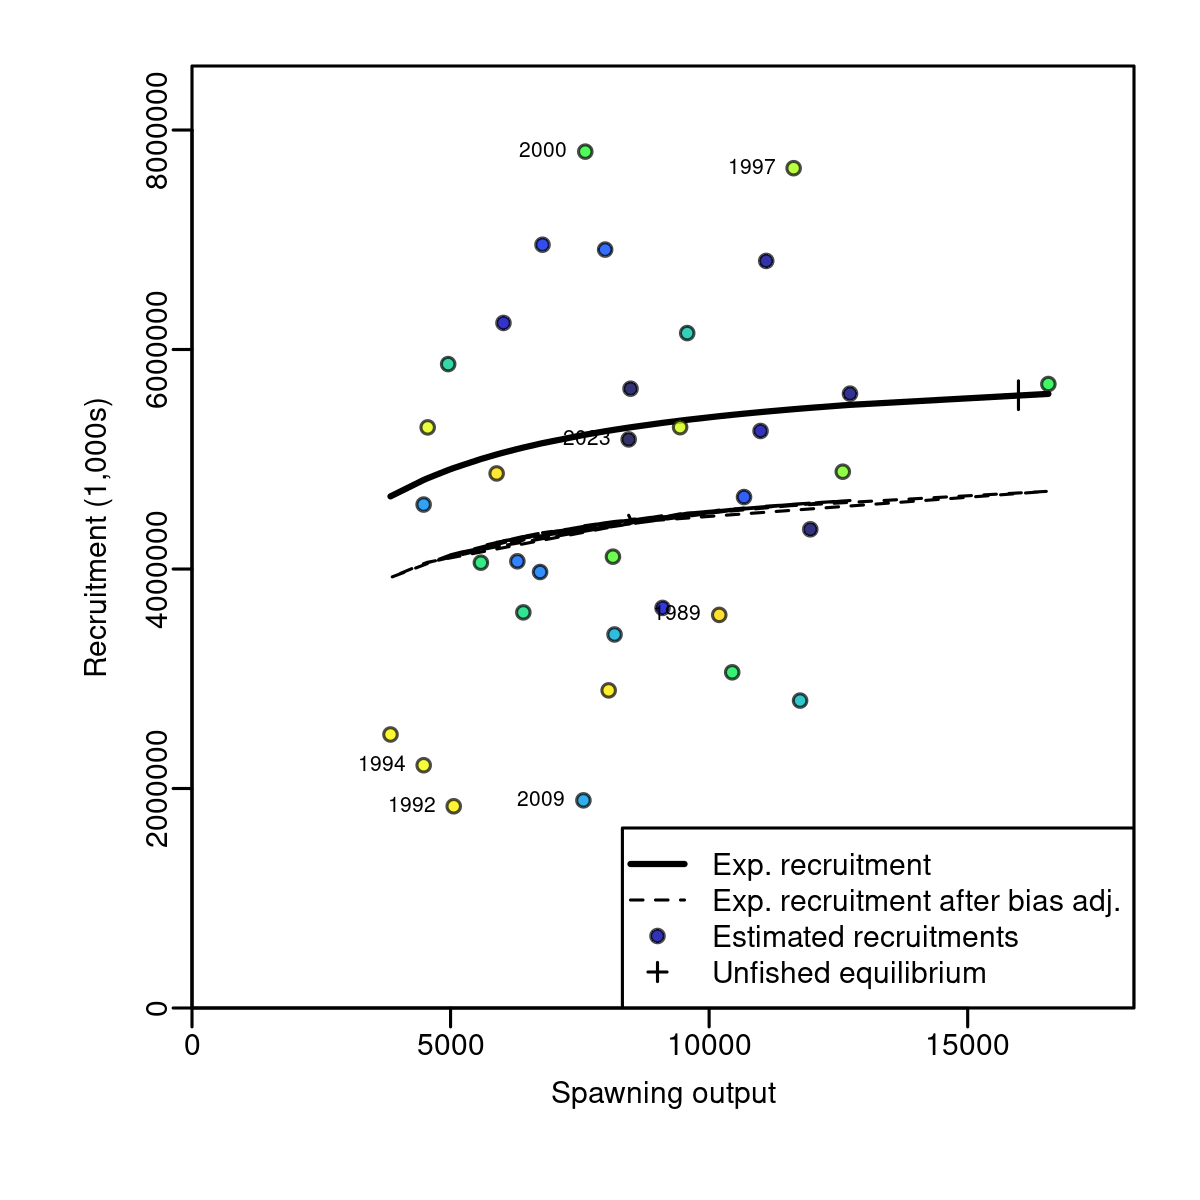
\includegraphics[width=0.95\linewidth]{report/run/S1.0_4FLEETS/fig_stock-recluta} 

}

\caption{ane.27.9a stock. Stock-recruit curve with labels on first, last, and years with (log) deviations > 0.5. Point colors indicate year, with warmer colors indicating earlier years and cooler colors in showing later years..}\label{fig:unnamed-chunk-31}
\end{figure}

\hypertarget{selectivity-1}{%
\subsection{Selectivity}\label{selectivity-1}}

Figure 25 shows the estimated selectivity for the age composition of the
commercial fleet and acoustic surveys (logistic-shaped fixed selectivity
across all years).

\begin{figure}[H]

{\centering 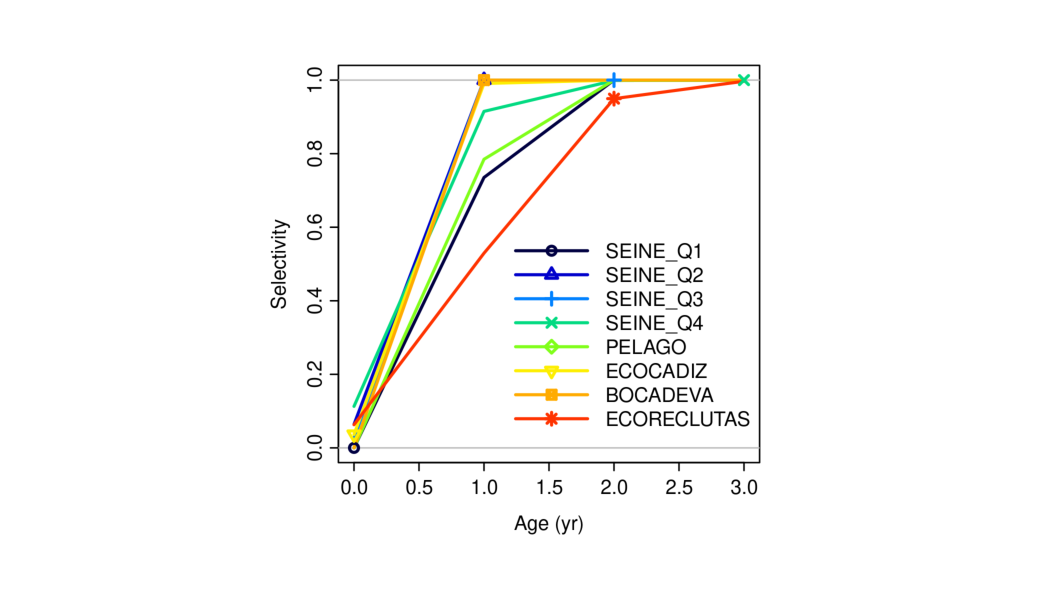
\includegraphics[width=0.95\linewidth]{Report_SS3_quarter_with_age_data_S1.0_4FLEETS_files/figure-latex/unnamed-chunk-32-1} 

}

\caption{ane.27.9a stock.Estimated selectivity for catch-at-age (logistic shaped fixed selectivity across all years).}\label{fig:unnamed-chunk-32}
\end{figure}

\hypertarget{catchability-1}{%
\subsection{Catchability}\label{catchability-1}}

The catchability (q) is adjusted to maintain a consistent relationship
between the observed biomass and the vulnerable biomass in acoustic
surveys. As vulnerable biomass decreases throughout the year,
catchability increases, indicating that efforts intensify when the
vulnerable biomass is lower (Figure 25 ).

\begin{figure}[H]

{\centering 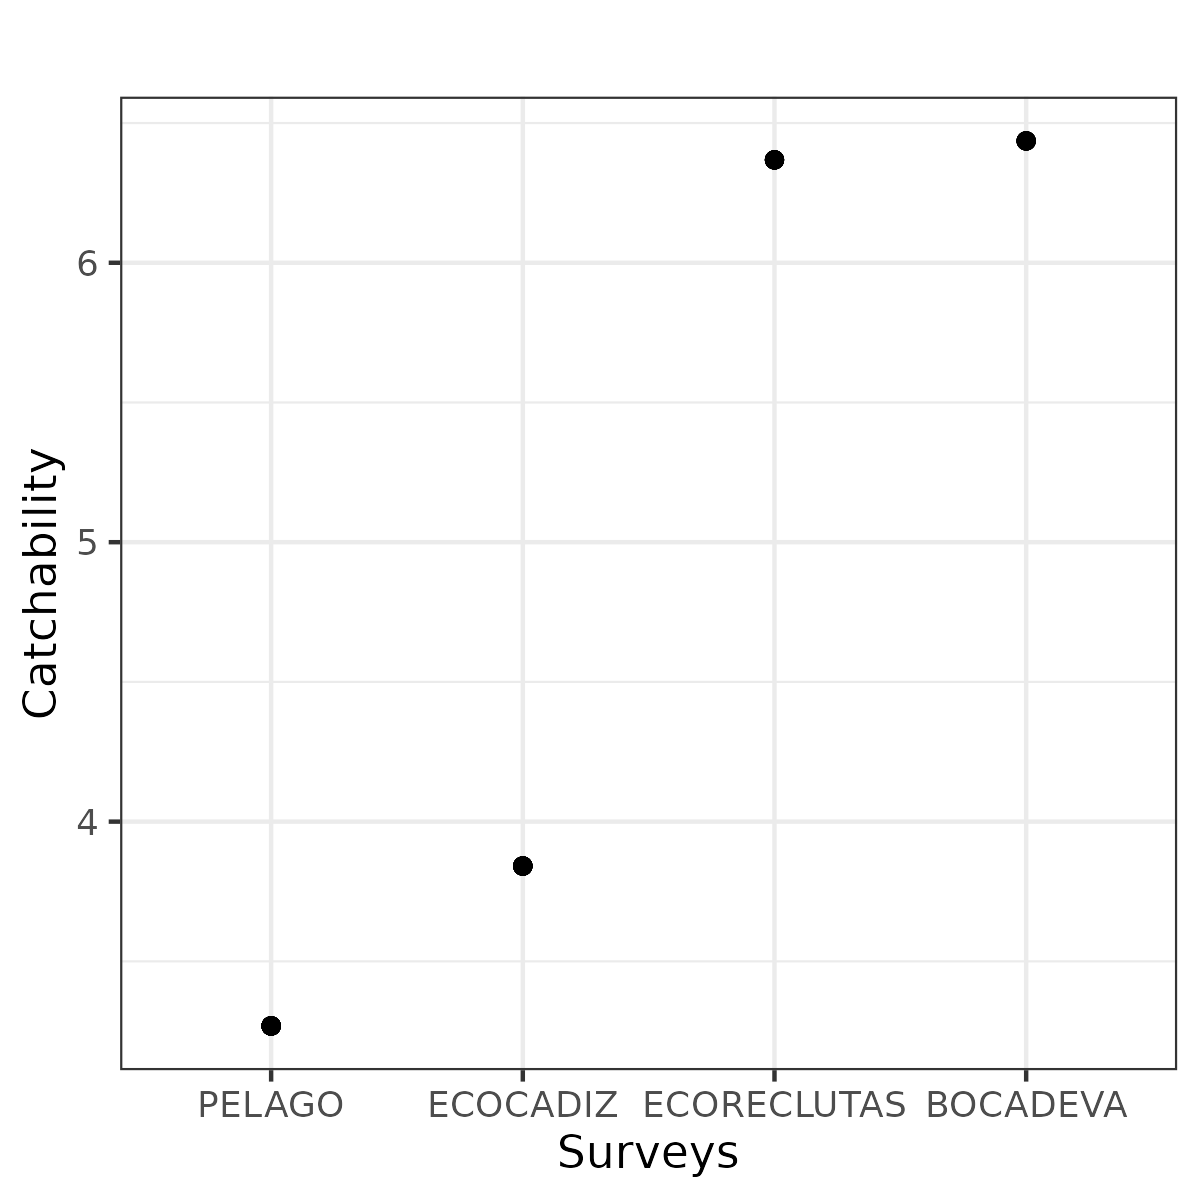
\includegraphics[width=0.95\linewidth]{report/run/S1.0_4FLEETS/fig_catchability} 

}

\caption{ane.27.9a stock. Estimated catchability parameters for the different surveys indices.}\label{fig:unnamed-chunk-33}
\end{figure}

\hypertarget{estimated-time-series}{%
\subsection{Estimated time series}\label{estimated-time-series}}

The Figure 26 shows that biomass fluctuates around a historical mean of
10.51 thousand tonnes, with a minimum in 1995 of 5.29 thousand tonnes
and a maximum recorded in 2001 of 18.73 thousand tonnes. In 2023, the
biomass is estimated to be -2\% below the historical mean. The catch
shows variability around the historical mean of 5.22 thousand tonnes,
with a maximum value recorded in 1998 of 9.6 thousand tonnes and a
minimum in 1995 of 0.57 thousand tonnes. In 2023, the catch is estimated
to be 42\% above the historical mean.

The fishing mortality (\(F_t\)) fluctuates around a historical mean of
1.11, with a maximum value recorded in 2023 of 1.85 and a minimum in
1995 of 0.16. Confidence intervals range from 0.21 to 0.03, with an
average of 0.12. The \(F_{2023}\) is estimated to be 67\% above the
historical mean.

The recruitment (\(R_t\)) fluctuates around a historical mean of 4.67
millions recruits, with a maximum value recorded in 2000 of 7.8 millions
recruits and a minimum in 1992 of 1.84 millions recruits. Confidence
intervals range from 0.23 to 0.03, with an average of 0.11. The
\(R_{2023}\) is estimated to be -11\% below the historical mean.

Finally, the spawning biomass (\(SSB_{t}\)) varies around a historical
mean of 8.41 thousand tonnes, with a maximum value recorded in 2001 of
16.56 thousand tonnes and a minimum in 1993 of 3.84 thousand tonnes.
Confidence intervals range from 0.22 to 0.03, with an average of 0.1.The
\texttt{SSB\_\{2023\}} is estimated to be 0\% below the historical mean.

The summarised results of the stock assessment are shown in Figure 26.

\begin{figure}[H]

{\centering 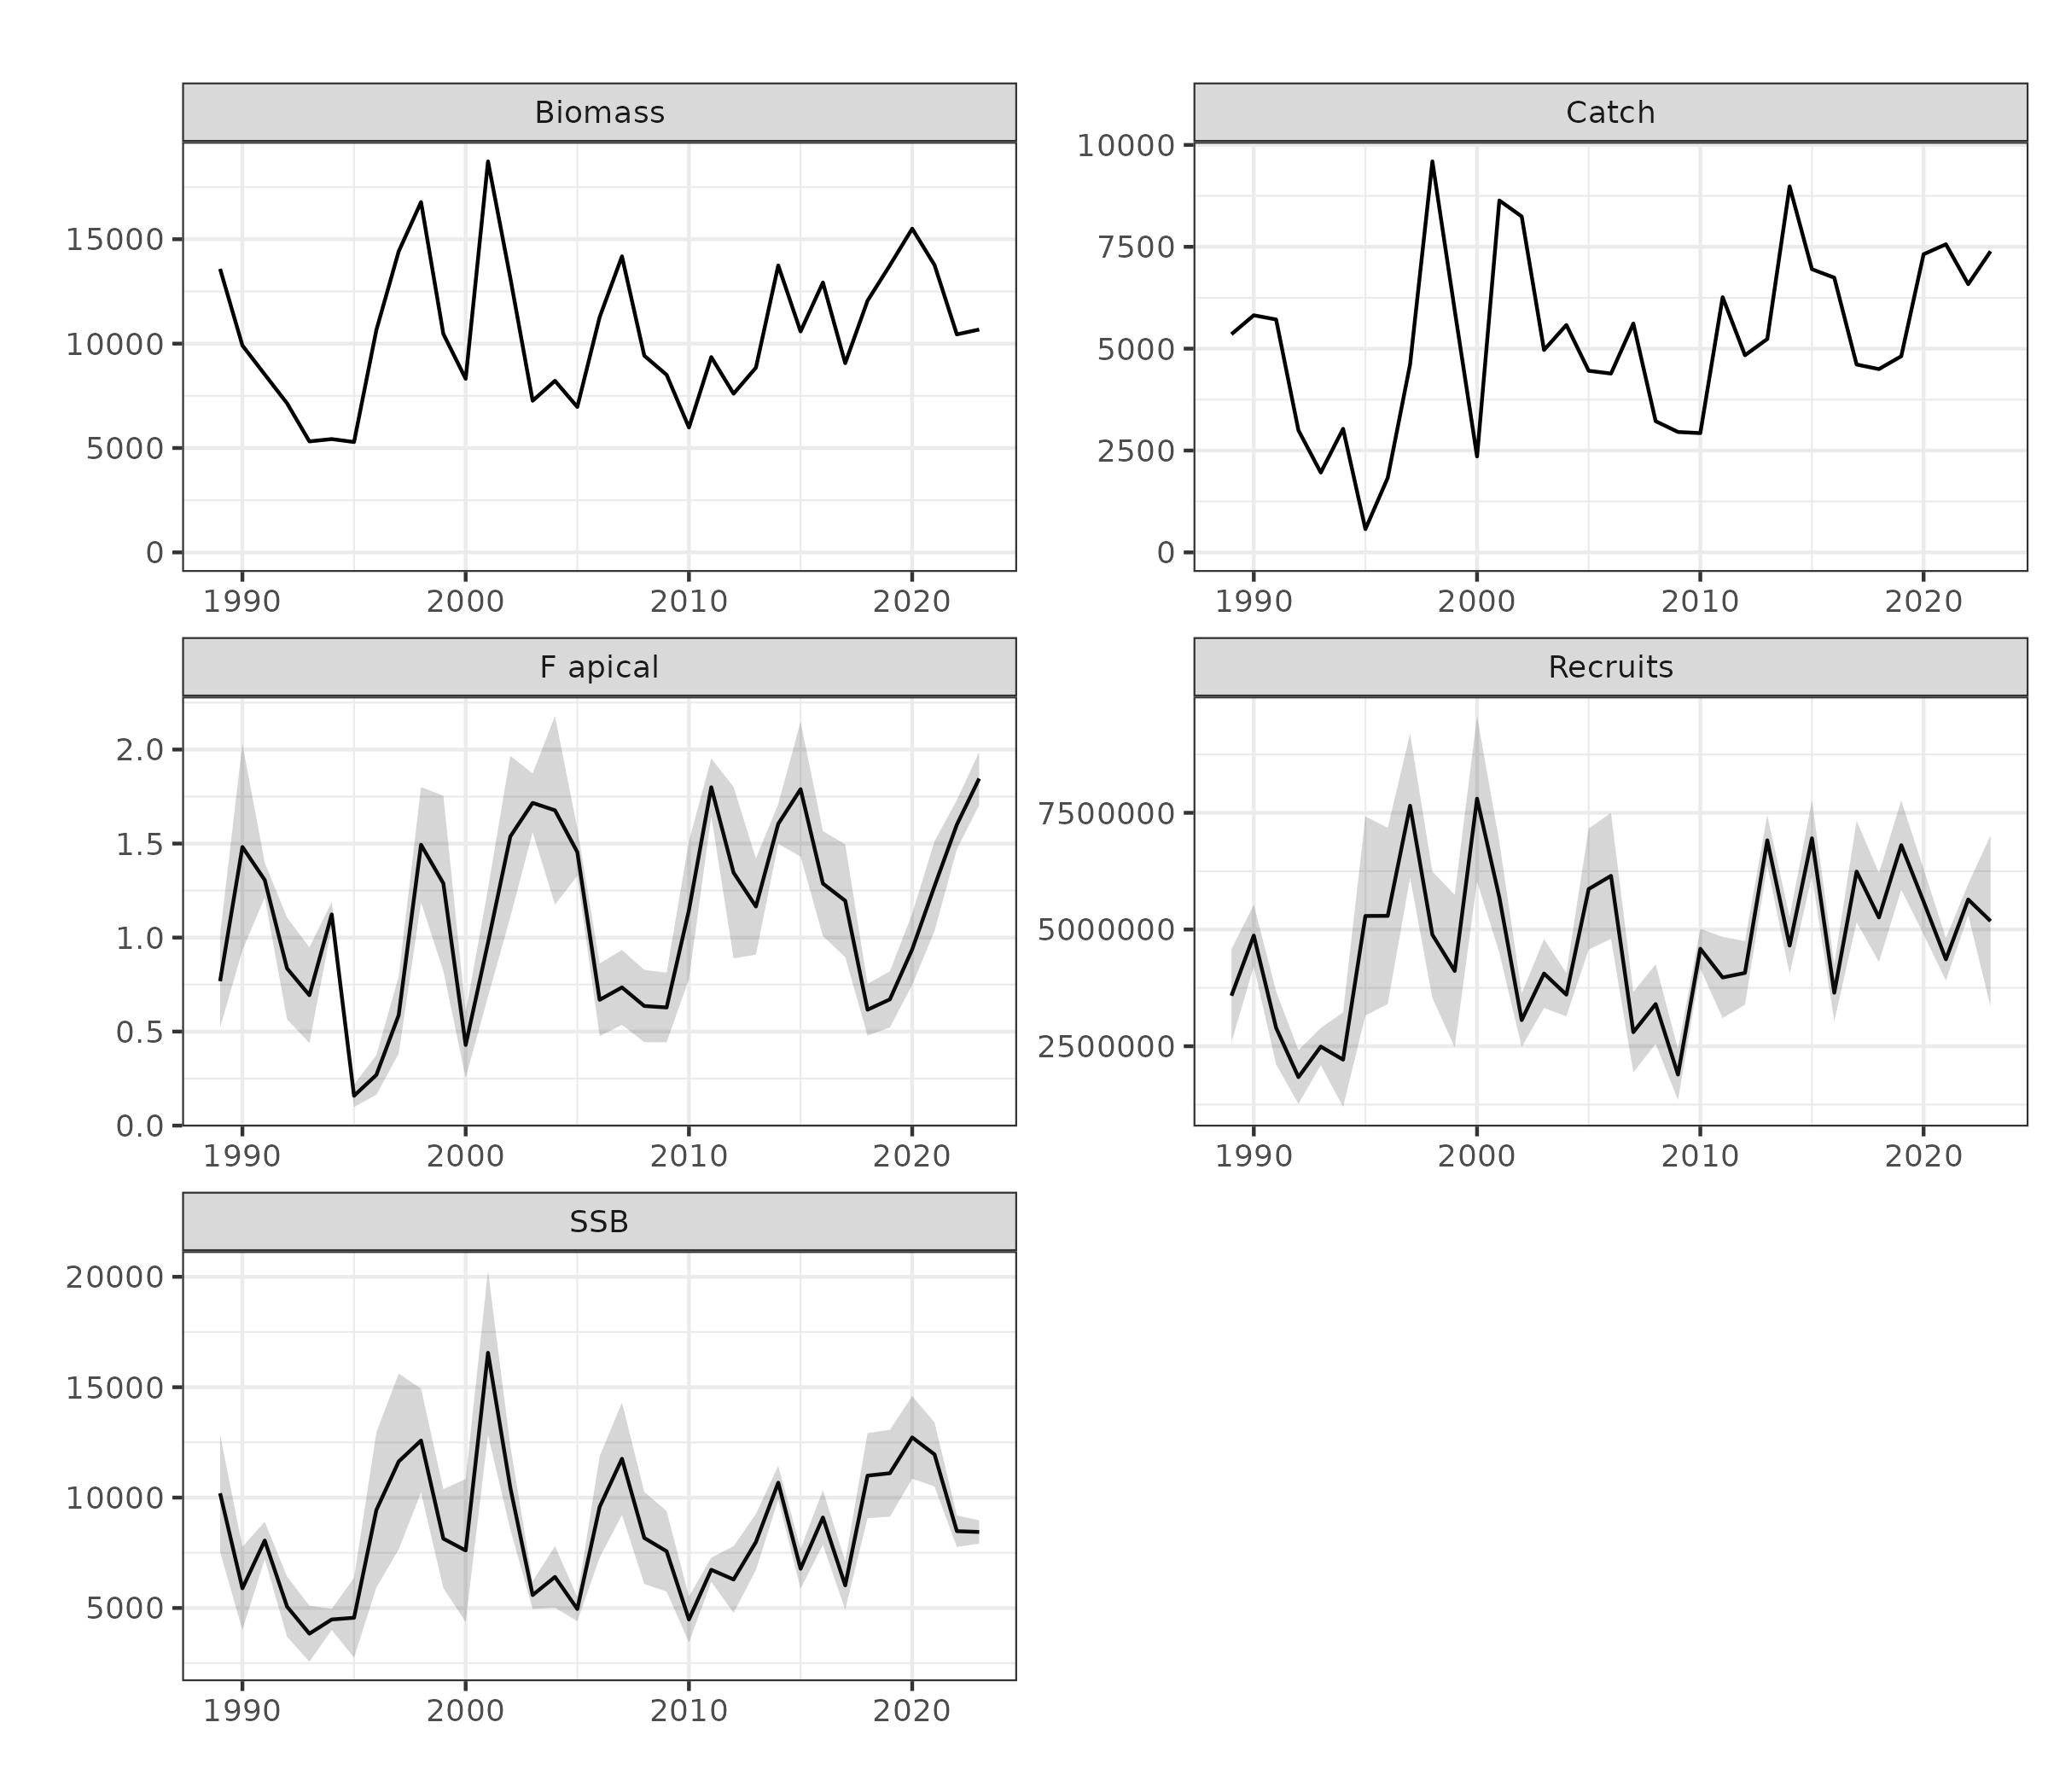
\includegraphics[width=0.95\linewidth]{report/run/S1.0_4FLEETS/fig_time_series} 

}

\caption{ane.27.9a stock. Time series estimated by the model for annual catches (in tons), recruitment (millions of fish), total biomass and spawning biomass (in tons), and fishing mortality (year-1).}\label{fig:unnamed-chunk-34}
\end{figure}

\begin{figure}[H]

{\centering 
\includegraphics[width=0.95\linewidth]{report/run/S1.0_4FLEETS/tb_timeseries} 

}

\caption{ane.27.9a stock. Time series estimated by the model for annual catches (in tons), recruitment (millions of fish), total biomass and spawning biomass (in tons), and fishing mortality (year-1).}\label{fig:unnamed-chunk-35}
\end{figure}

\hypertarget{acknowledgements}{%
\section{Acknowledgements}\label{acknowledgements}}

Financial support was received for the work developed in this document.
In particular, M. José Zúñiga work was funded by the Math4Fish project:
New tools for mathematical modelling in Spanish fisheries scientific
advice, financed by the European Union -- NextGenerationEU, and the
Recovery and Resilience Facility, Component 3, Investment 7 and has been
carried out within the framework of the agreement between the Spanish
Ministry of Agriculture, Fishing and Food and the Spanish National
Research Council (CSIC) through the Spanish Institute of Oceanography
(IEO) to promote fisheries research as a basis for sustainable fisheries
management. Views and opinions expressed are however those of the
author(s) only and do not necessarily reflect those of the European
Union or European Commission. Neither the European Union nor the
European Commission can be held responsible for them.

Additionally, this work would have not been possible without the
collection of Spanish fisheries and surveys data, co-funded by the
Spanish Institute of Oceanography (IEO) and the EU through the European
Maritime and Fisheries Fund (EMFF) within the National Program of
collection, management and use of data in the fisheries sector and
support for scientific advice regarding the Common Fisheries Policy
(PNDB/EU-DCF-Programa Nacional de Datos Básicos/EU-Data Collection
Framework).

\hypertarget{references}{%
\section*{References}\label{references}}
\addcontentsline{toc}{section}{References}

\hypertarget{refs}{}
\begin{CSLReferences}{1}{0}
\leavevmode\vadjust pre{\hypertarget{ref-Carvalho2021}{}}%
Carvalho, F., Winker, H., Courtney, D., Kapur, M., Kell, L., Cardinale,
M., Schirripa, M., \emph{et al.} 2021. A cookbook for using model
diagnostics in integrated stock assessments. Fisheries Research, 240:
105959.
\url{https://www.sciencedirect.com/science/article/pii/S0165783621000874}.

\leavevmode\vadjust pre{\hypertarget{ref-Francis2011}{}}%
Francis, R. I. C. C. 2011. Data weighting in statistical fisheries stock
assessment models. Canadian Journal of Fisheries and Aquatic Sciences,
68: 1124--1138.\href{\%20https://doi.org/10.1139/f2011-025}{
https://doi.org/10.1139/f2011-025}.

\leavevmode\vadjust pre{\hypertarget{ref-Hsu2024}{}}%
Hsu, J., Chang, Y.-J., Brodziak, J., Kai, M., and Punt, A. E. 2024. {On
the probable distribution of stock-recruitment resilience of Pacific
saury (Cololabis saira) in the Northwest Pacific Ocean}. ICES Journal of
Marine Science, 81: 748--759.
\url{https://doi.org/10.1093/icesjms/fsae030}.

\leavevmode\vadjust pre{\hypertarget{ref-HurtadoFerro2014}{}}%
Hurtado-Ferro, F., Szuwalski, C. S., Valero, J. L., Anderson, S. C.,
Cunningham, C. J., Johnson, K. F., Licandeo, R., \emph{et al.} 2014.
{Looking in the rear-view mirror: bias and retrospective patterns in
integrated, age-structured stock assessment models}. ICES Journal of
Marine Science, 72: 99--110.
\url{https://doi.org/10.1093/icesjms/fsu198}.

\leavevmode\vadjust pre{\hypertarget{ref-Methot2011}{}}%
Methot, R. D., and Taylor, I. G. 2011. Adjusting for bias due to
variability of estimated recruitments in fishery assessment models.
Canadian Journal of Fisheries and Aquatic Sciences, 68:
1744--1760.\href{\%20\%0A\%20\%20\%20\%20\%0A\%20\%20\%20\%20\%20\%20\%20\%20https://doi.org/10.1139/f2011-092\%0A\%20\%20\%20\%20\%0A\%20\%20\%20\%20\%0A\%0A}{
https://doi.org/10.1139/f2011-092 }.

\leavevmode\vadjust pre{\hypertarget{ref-Methot2013}{}}%
Methot, R. D., and Wetzel, C. R. 2013. Stock synthesis: A biological and
statistical framework for fish stock assessment and fishery management.
Fisheries Research, 142: 86--99.
\url{https://doi.org/10.1016/j.fishres.2012.10.012}.

\leavevmode\vadjust pre{\hypertarget{ref-Methot2024}{}}%
Methot, R. D., Wetzel, C. R., Taylor, I. G., Doering, K., Perl, E., and
K. Johnson. 2024. Stock synthesis user manual : Version 3.30.22.1.
\url{https://github.com/nmfs-ost/ss3-source-code/releases}.

\leavevmode\vadjust pre{\hypertarget{ref-Taylor2021}{}}%
Taylor, I. G., Doering, K. L., Johnson, K. F., Wetzel, C. R., and
Stewart, I. J. 2021. Beyond visualizing catch-at-age models: Lessons
learned from the r4ss package about software to support stock
assessments. Fisheries Research, 239: 105924.
\url{https://doi.org/10.1016/j.fishres.2021.105924}.

\leavevmode\vadjust pre{\hypertarget{ref-Wiff2018}{}}%
Wiff, R., Flores, A., Neira, S., and Caneco, B. 2018. Estimating
steepness of the stock-recruitment relationship in chilean fish stocks
using meta-analysis. Fisheries Research, 200: 61--67.
\url{https://www.sciencedirect.com/science/article/pii/S0165783617303399}.

\end{CSLReferences}

\end{document}
